%% TEXTURE IMAGES
%%
\begin{figure}[!ht]
\center 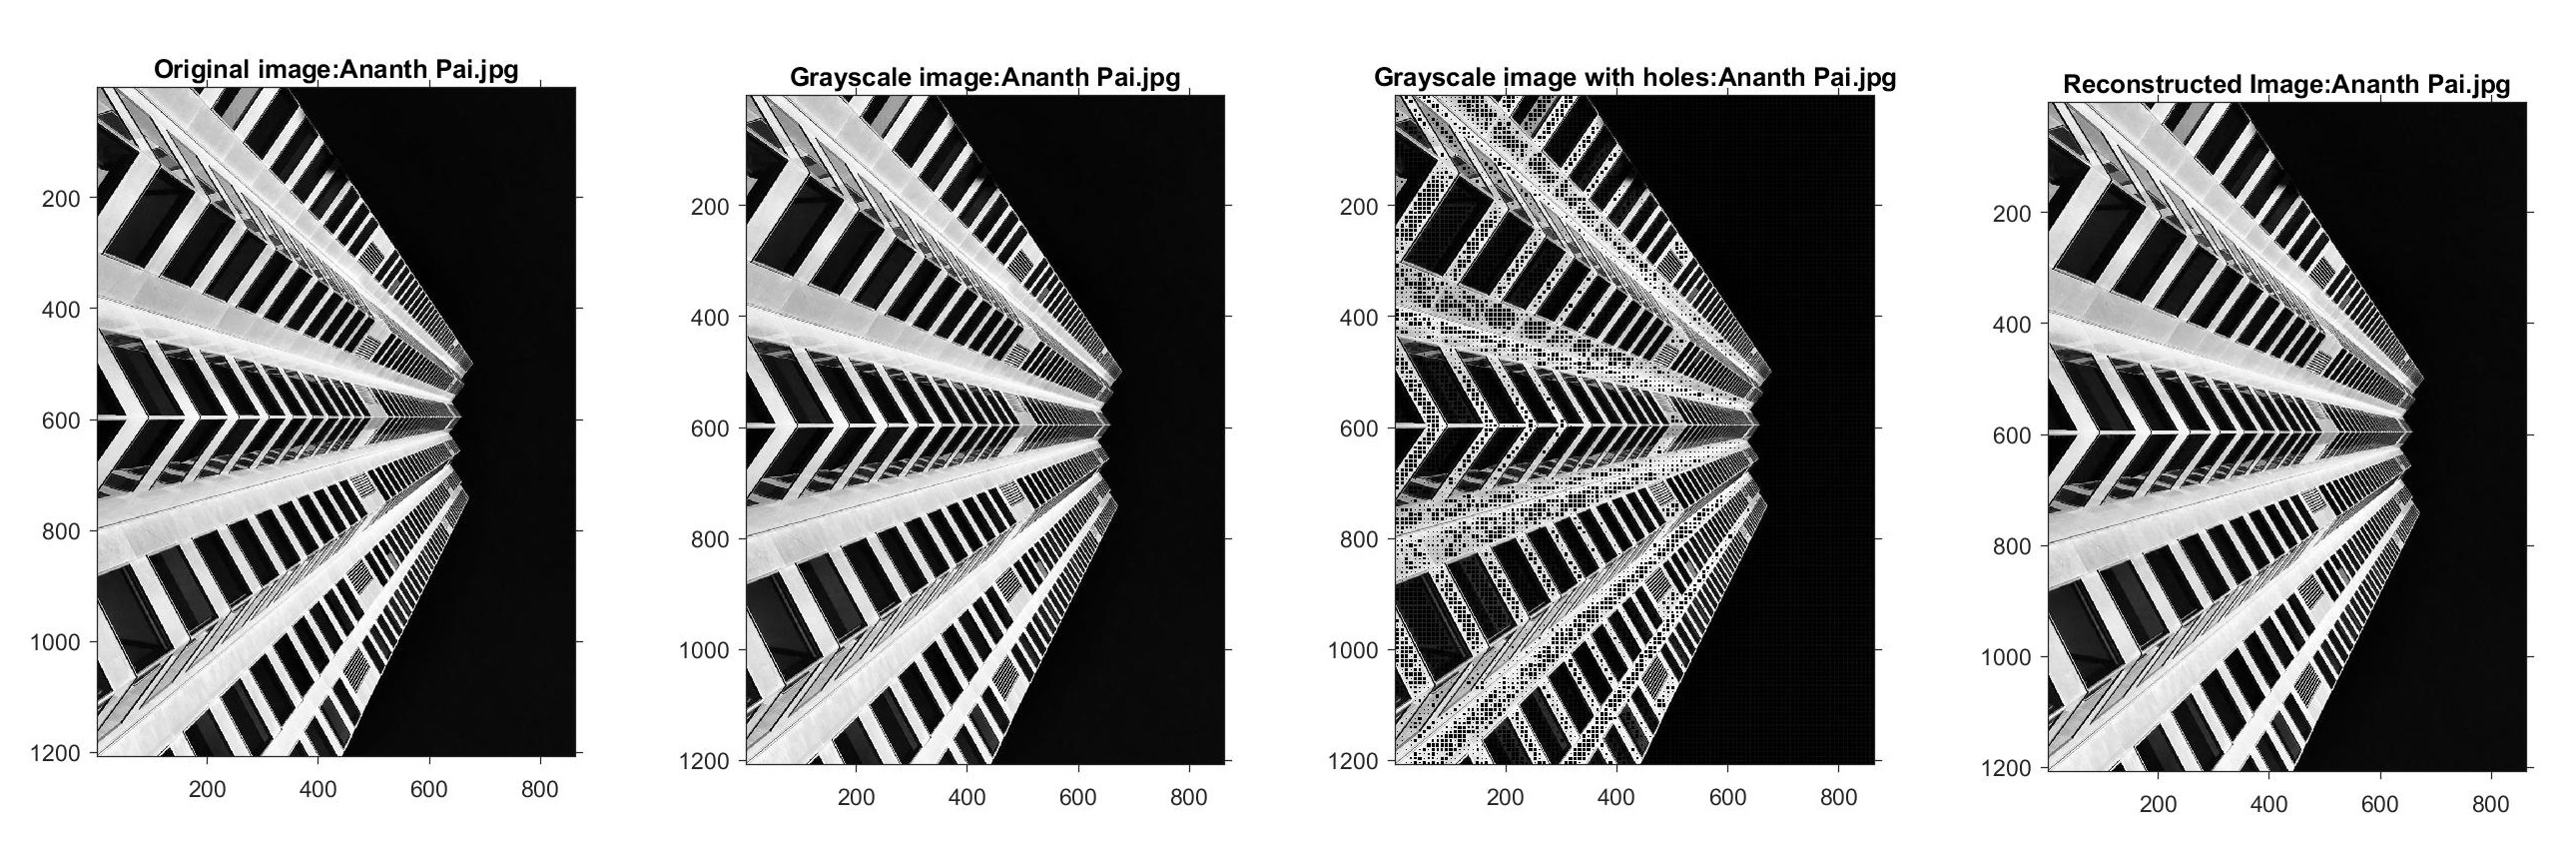
\includegraphics[scale=0.26]{AnanthPai.jpg}
\caption{Ananth Pai high contrast image with 0\% error introduction}
\label{fig:aphc}
\end{figure}

\begin{figure}[!ht]
\center 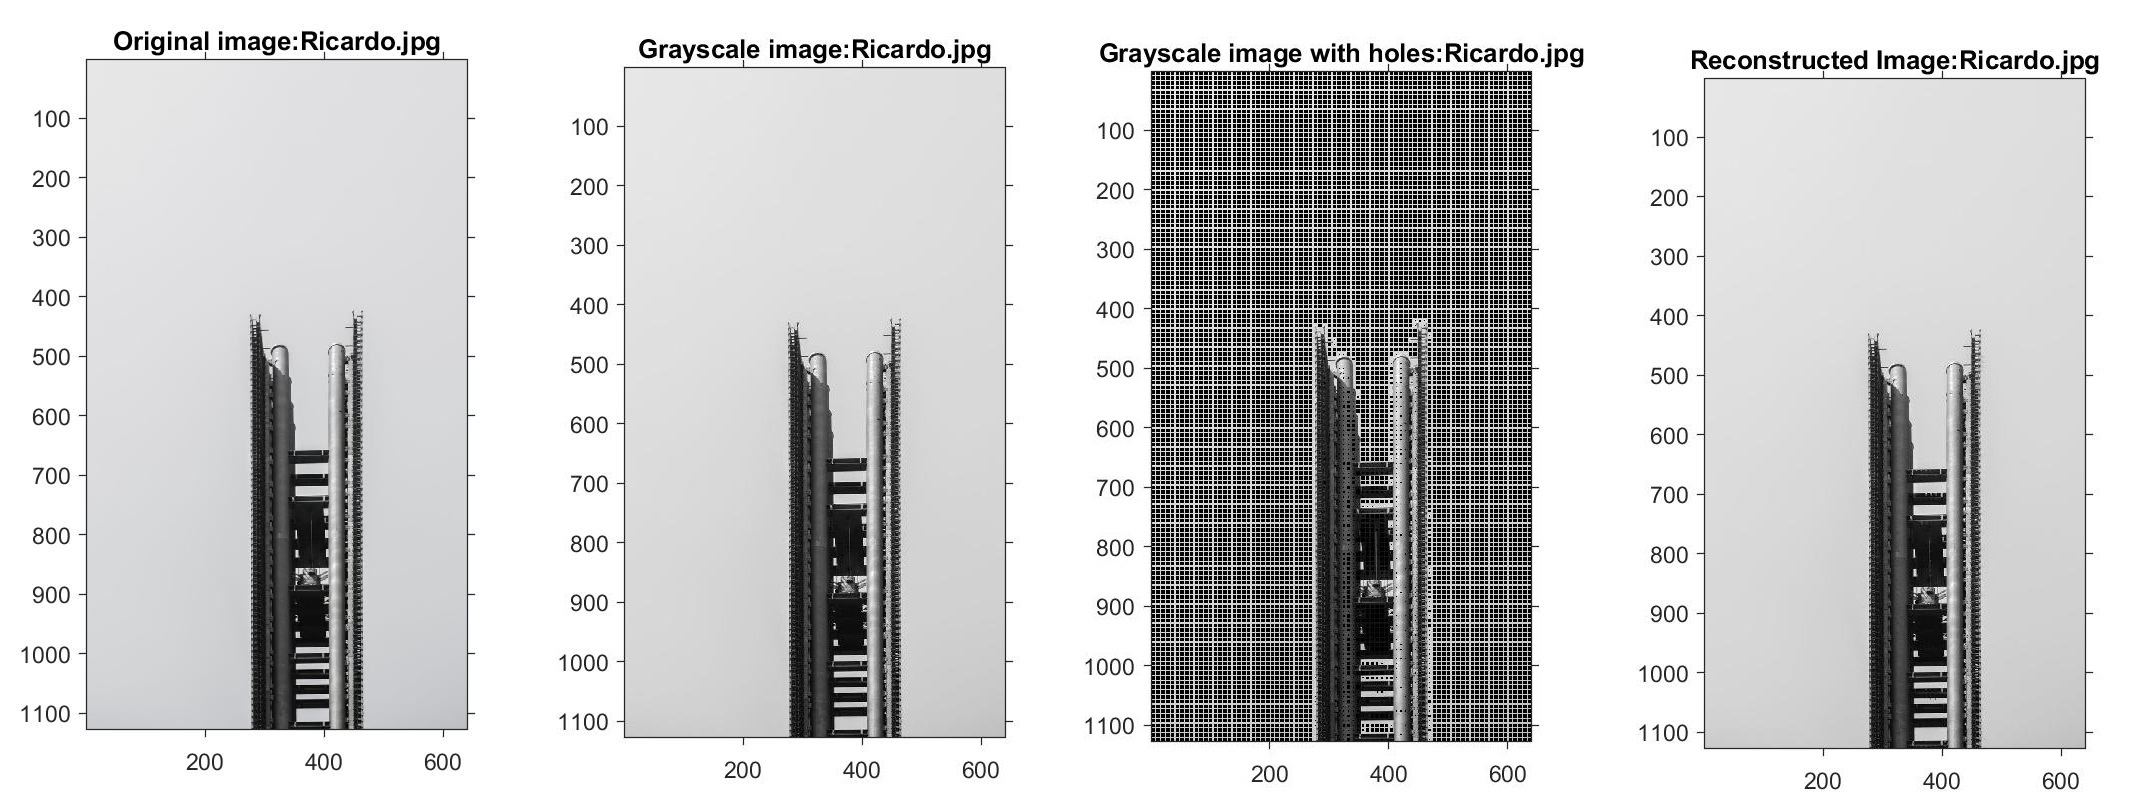
\includegraphics[scale=0.315]{Ricardo.jpg}
\caption{Ricardo high contrast image with 0\% error introduction}
\label{fig:rhc}
\end{figure}

\begin{figure}[!ht]
\center 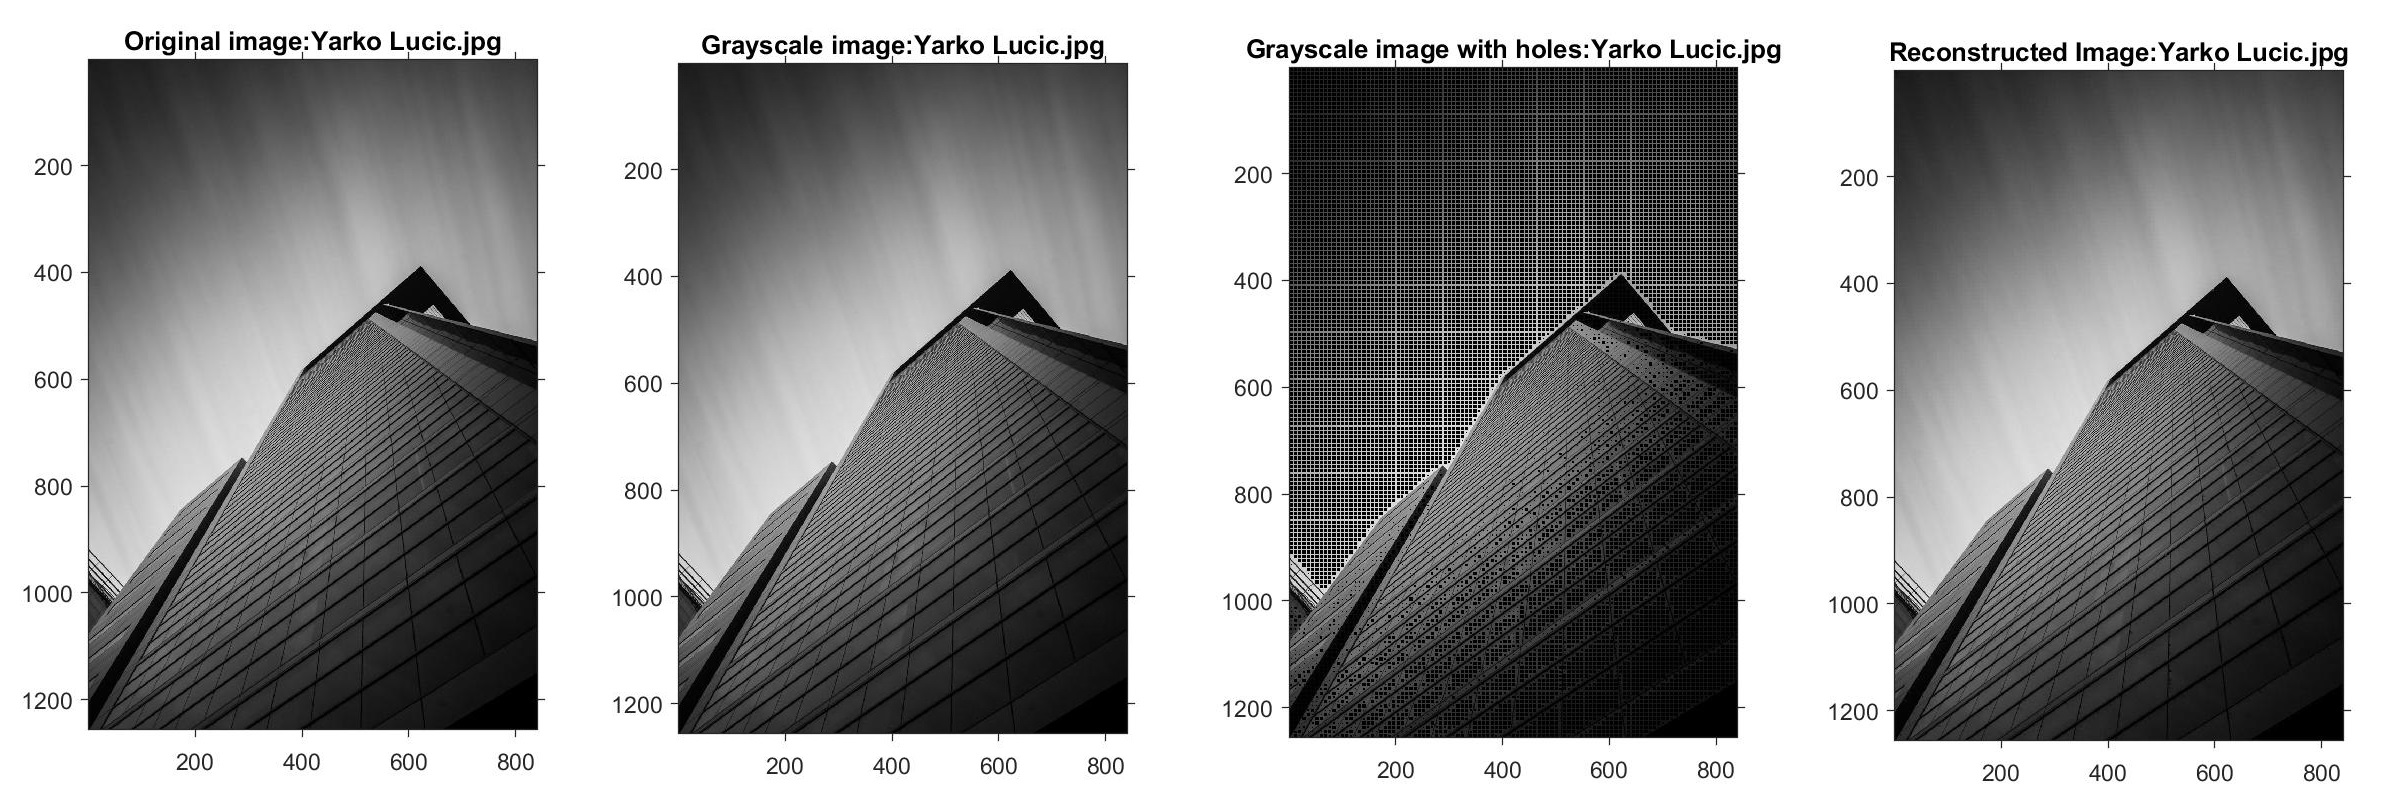
\includegraphics[scale=0.28]{YarkoLucic.jpg}
\caption{Yarko Lucic high contrast image with 0\% error introduction}
\label{fig:ylhc}
\end{figure}
%%

%% LANDSCAPE IMAGES
%%
\begin{figure}[!ht]
\center 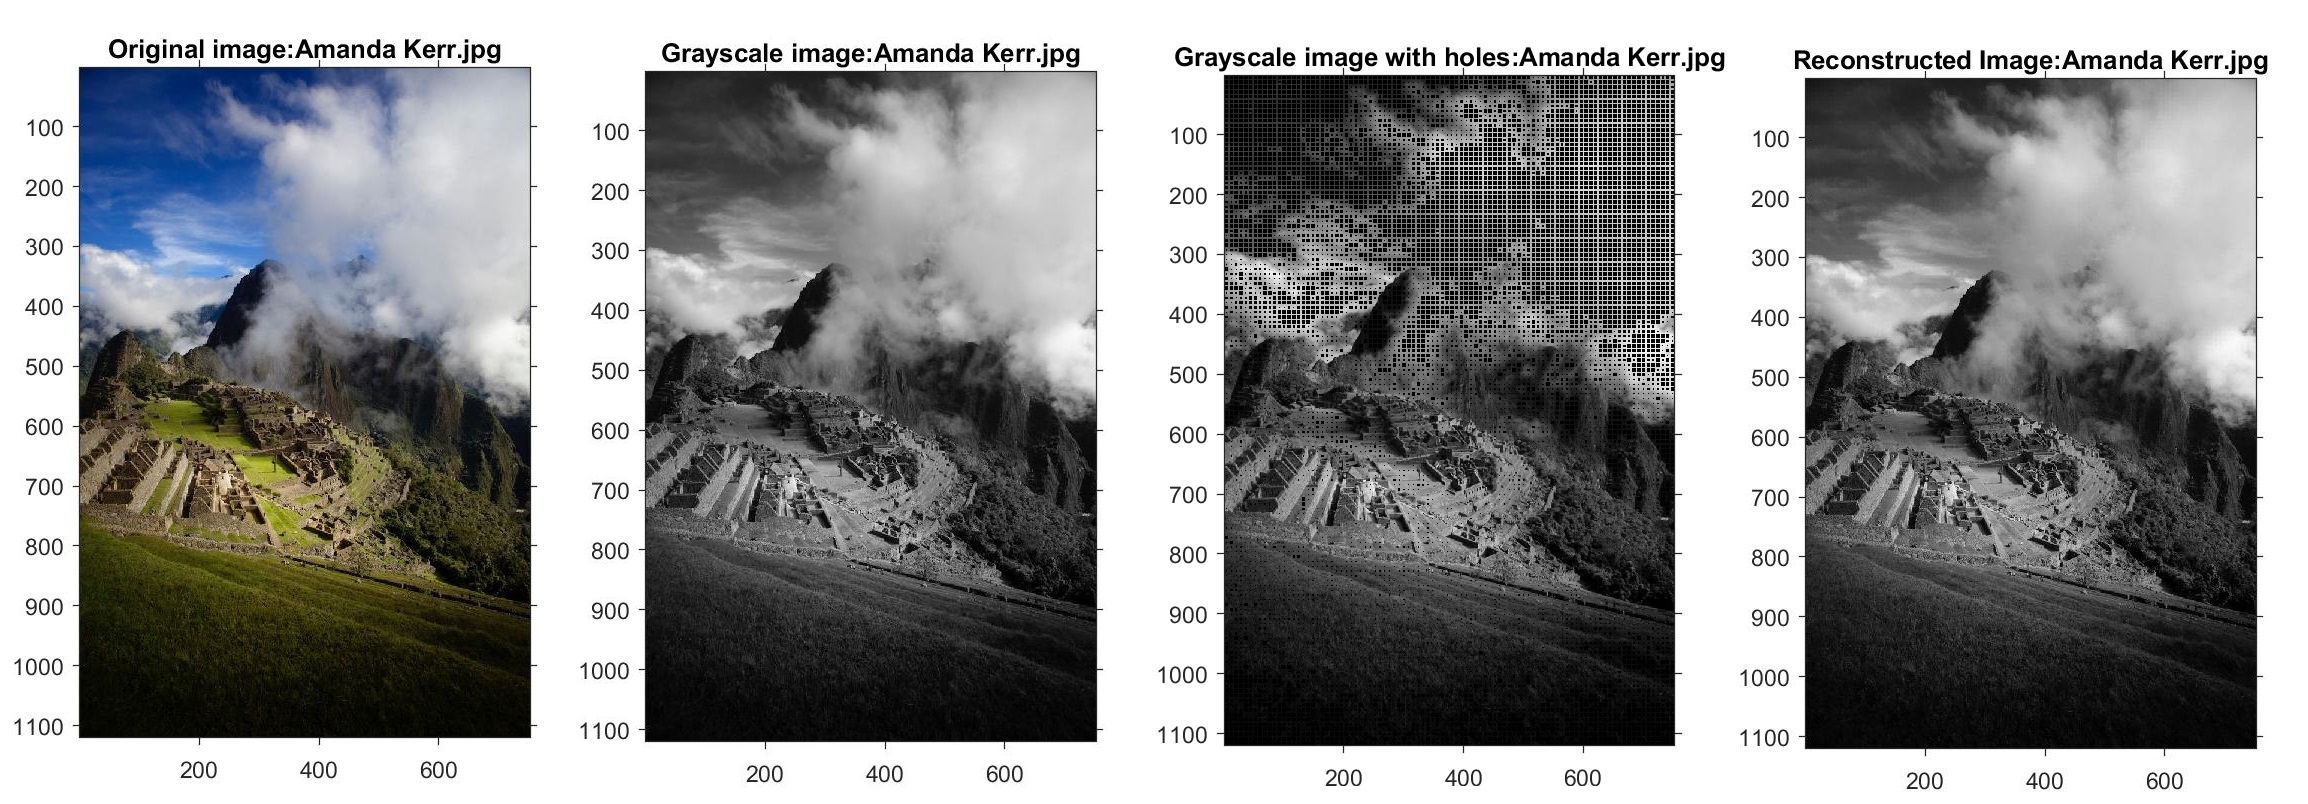
\includegraphics[scale=0.3]{AmandaKerr.jpg}
\caption{Amanda Kerr landscape image with 0\% error introduction}
\label{fig:akl}
\end{figure}

\begin{figure}[!ht]
\center 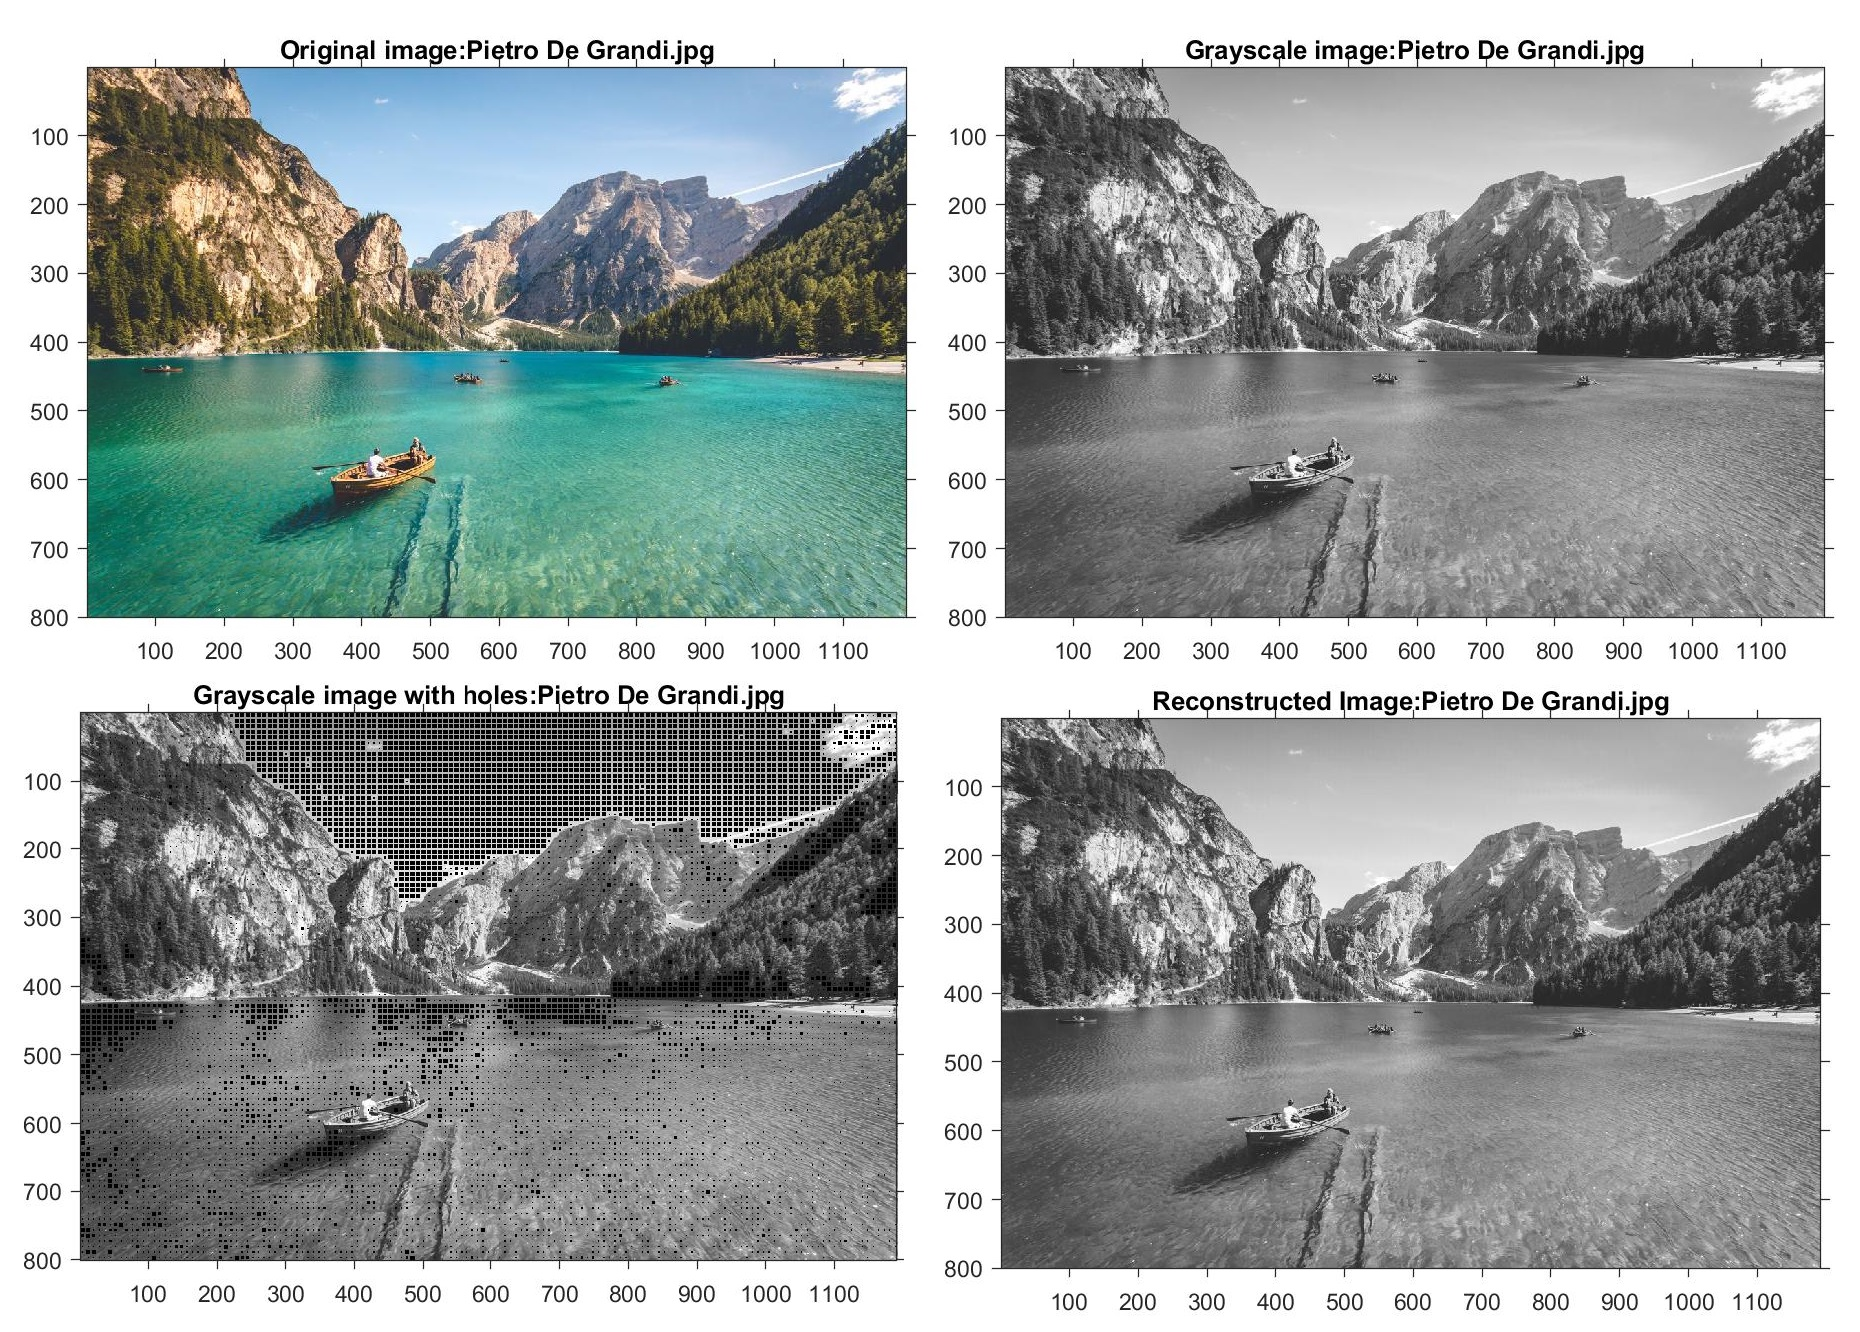
\includegraphics[scale=0.37]{PietroDiGrandi.jpg}
\caption{Pietro Di Grandi landscape image with 0\% error introduction}
\label{fig:pdgl}
\end{figure}

\begin{figure}[!ht]
\center 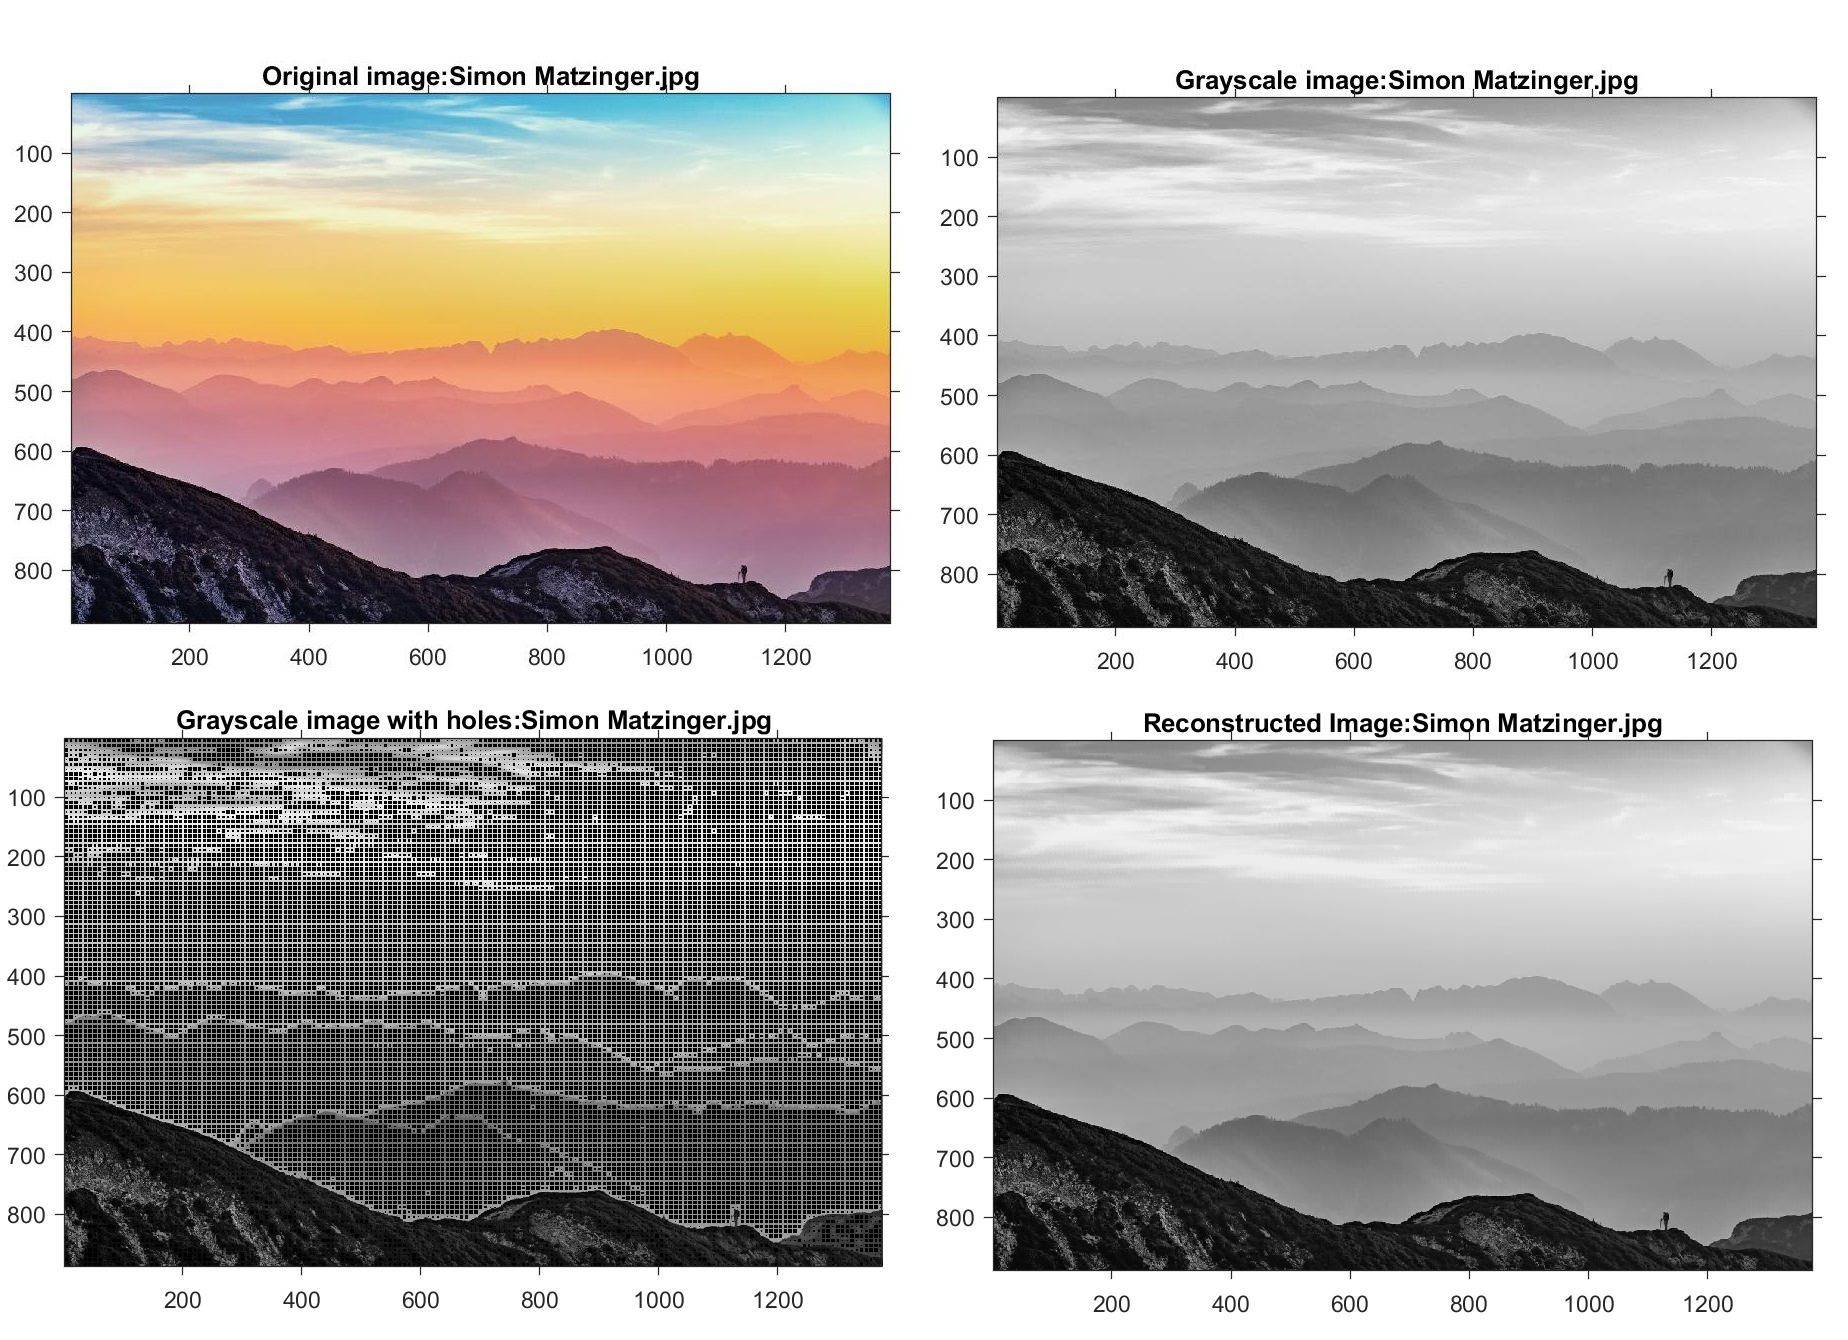
\includegraphics[scale=0.37]{SimonMatzinger.jpg}
\caption{Simon Matzinger landscape image with 0\% error introduction}
\label{fig:sml}
\end{figure}
%%

%% HIGH CONTRAST IMAGES
%%
\begin{figure}[!ht]
\center 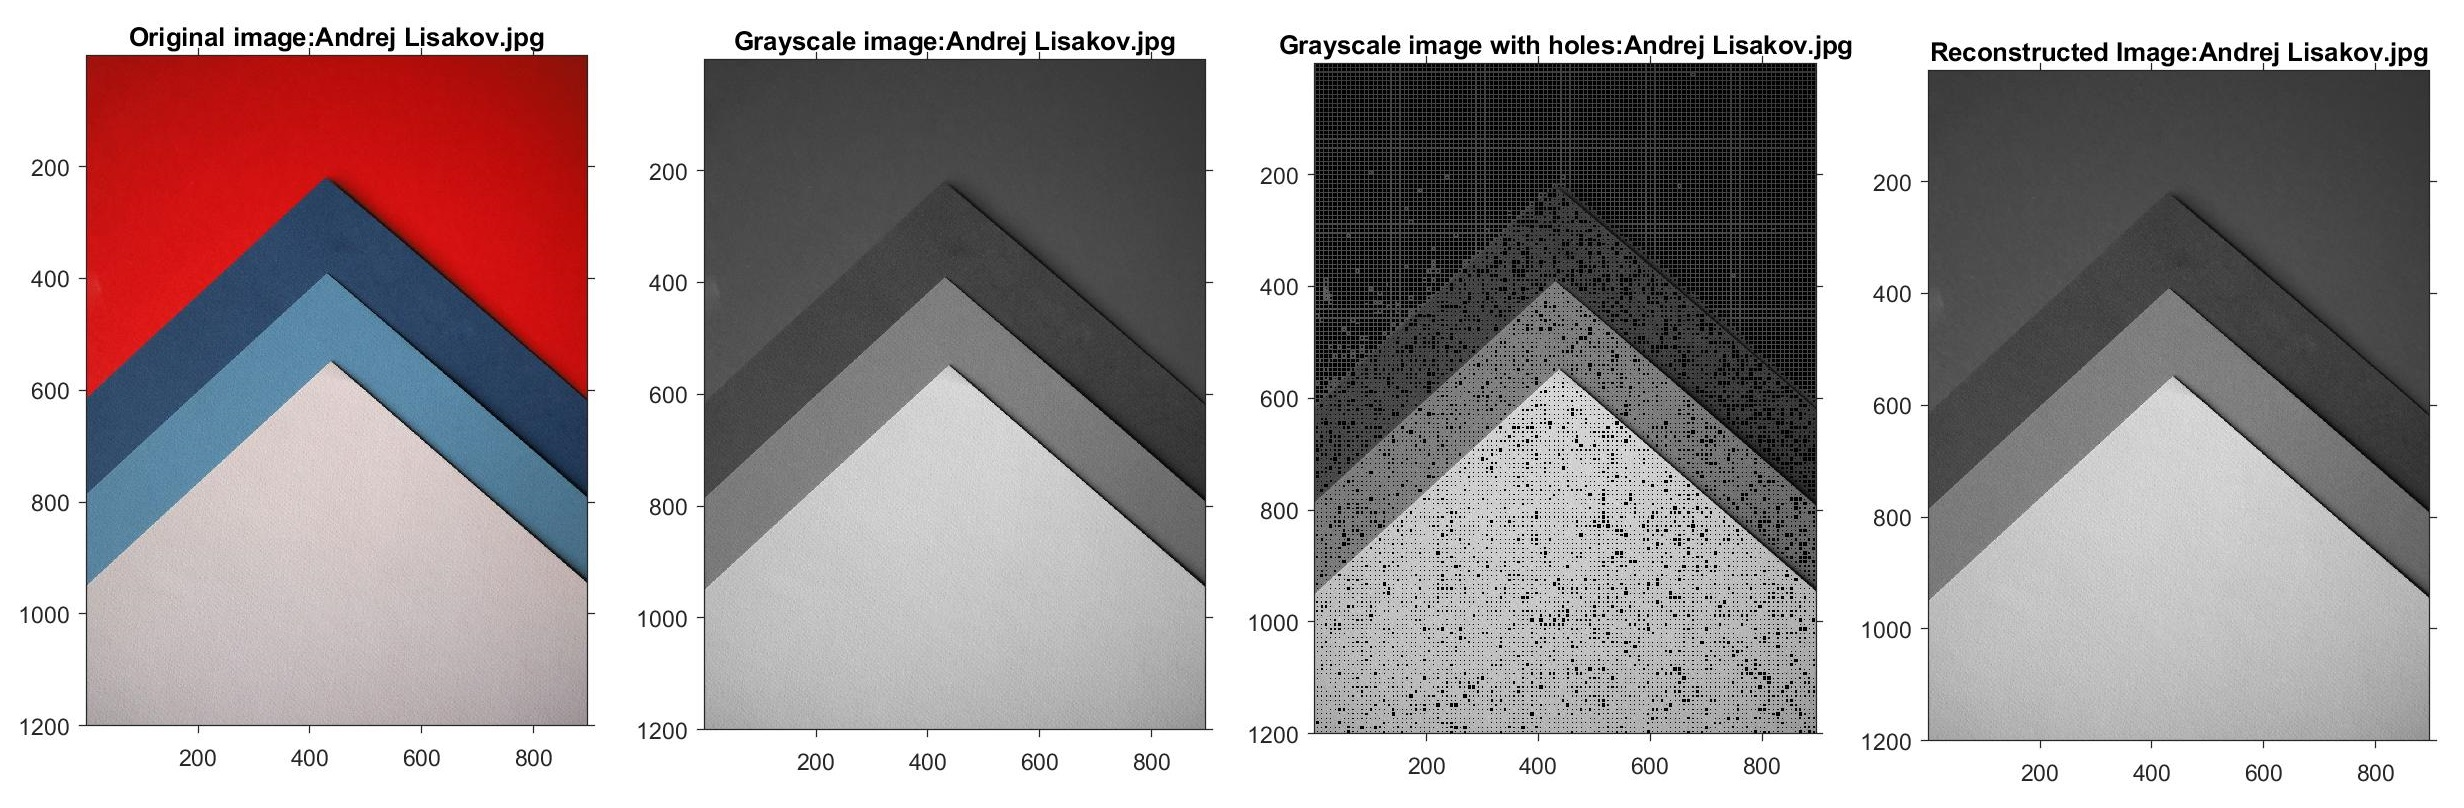
\includegraphics[scale=0.28]{AndrejLisakov.jpg}
\caption{Andrej Lisakov texture image with 0\% error introduction}
\label{fig:alt}
\end{figure}

\begin{figure}[!ht]
\center 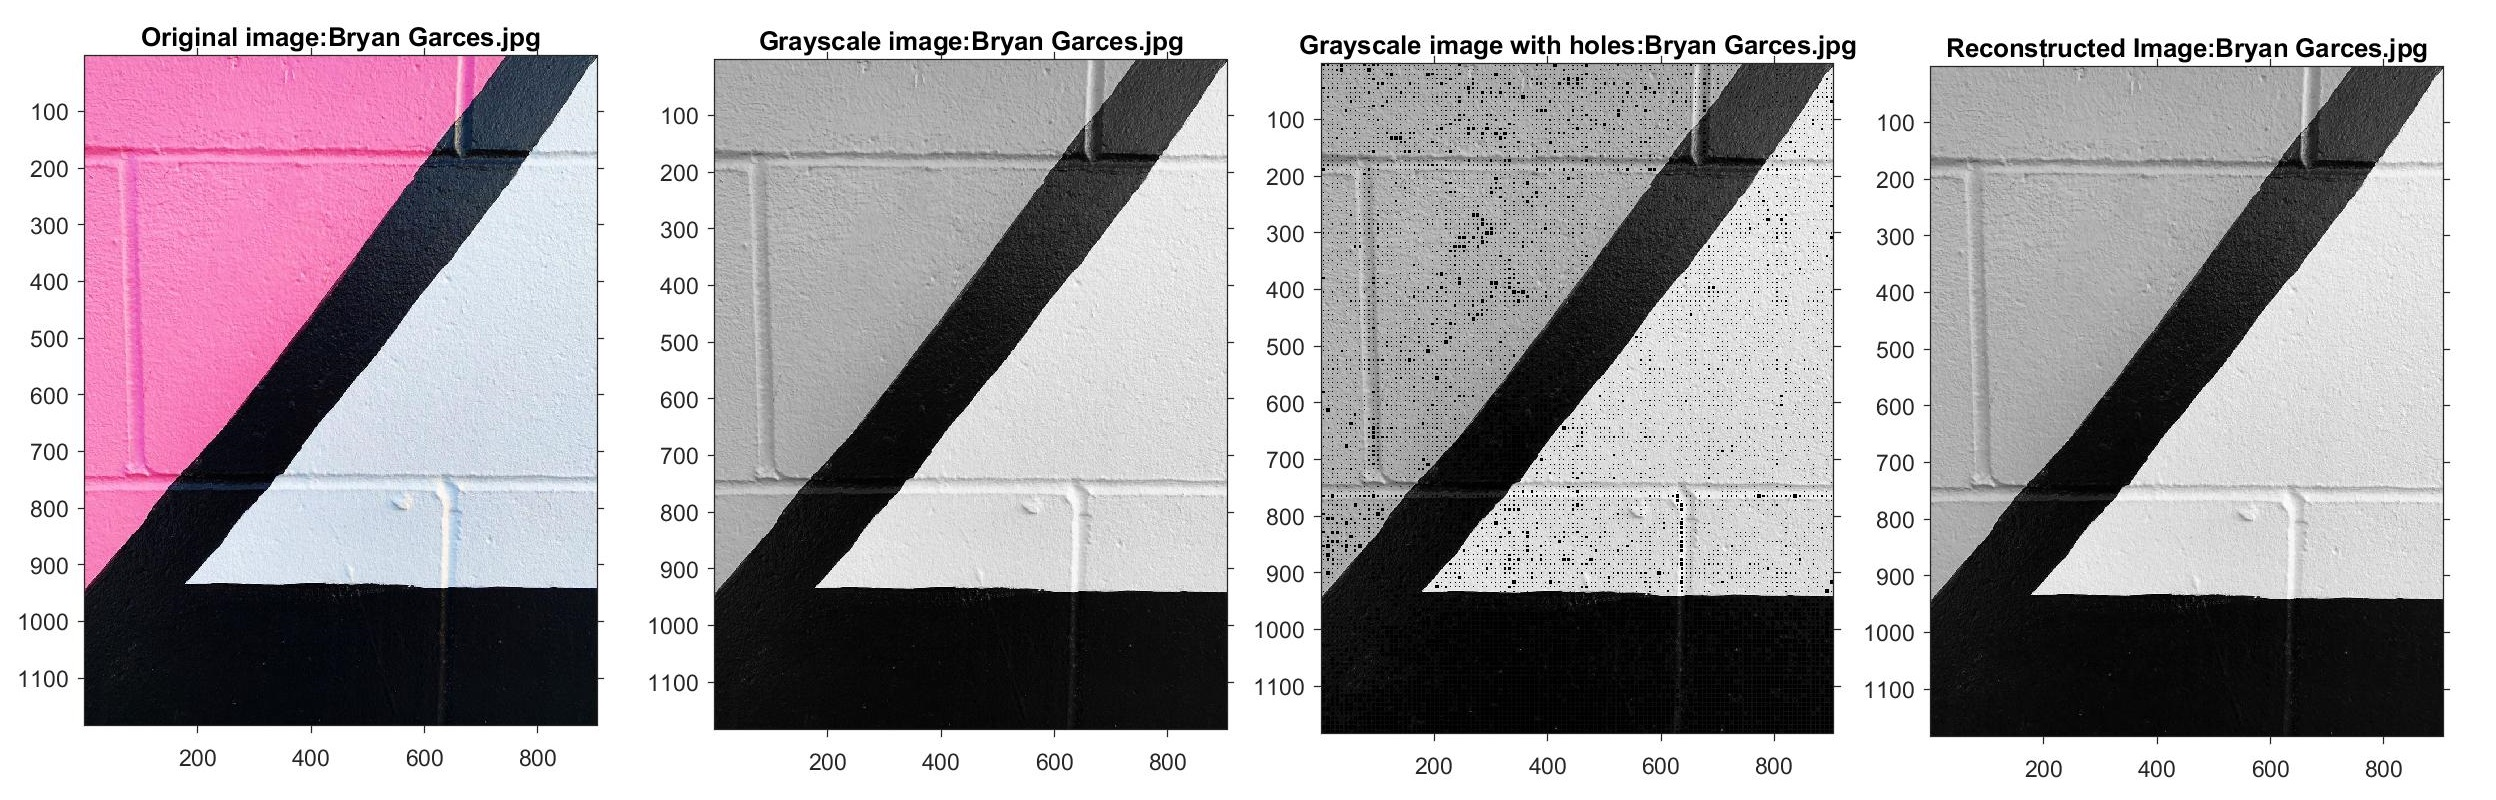
\includegraphics[scale=0.28]{BryanGarces.jpg}
\caption{Bryan Garces texture image with 0\% error introduction}
\label{fig:bgt}
\end{figure}

\begin{figure}[!ht]
\center 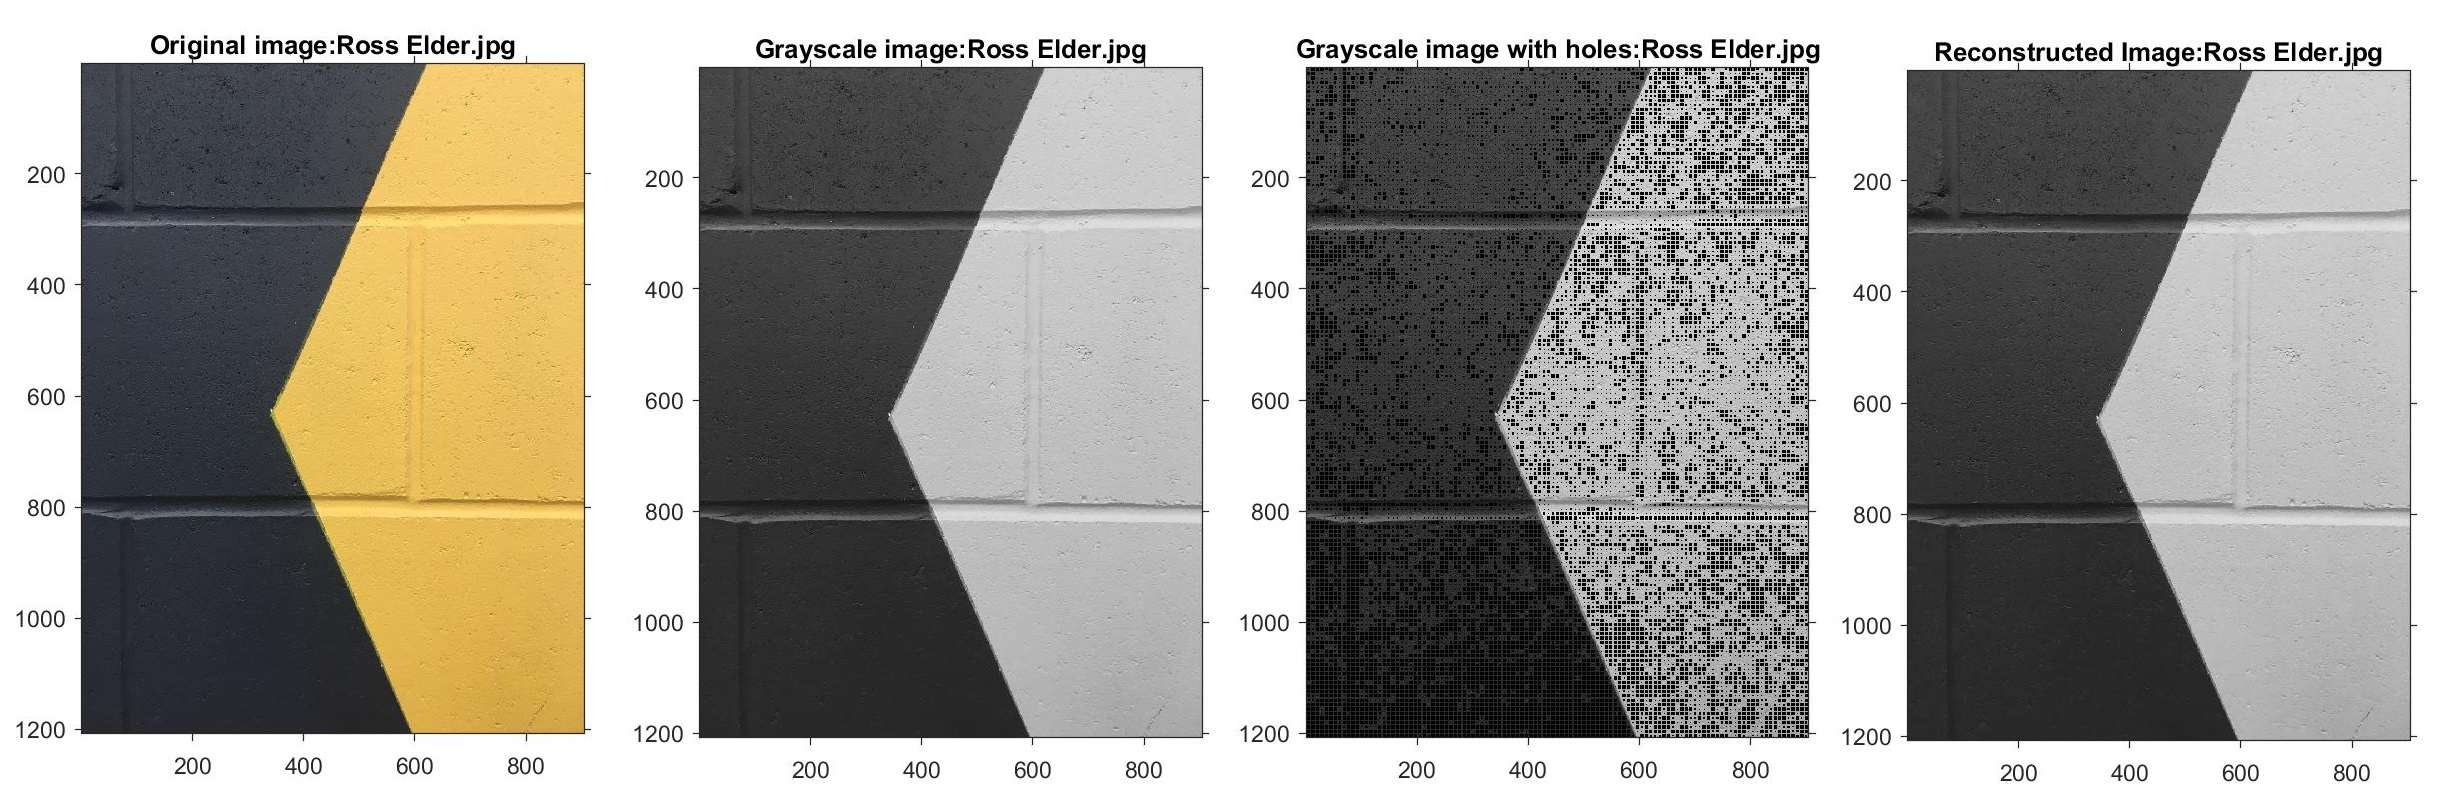
\includegraphics[scale=0.28]{RossElder.jpg}
\caption{Ross Elder texture image with 0\% error introduction}
\label{fig:ret}
\end{figure}

\begin{figure}[!ht]
\center 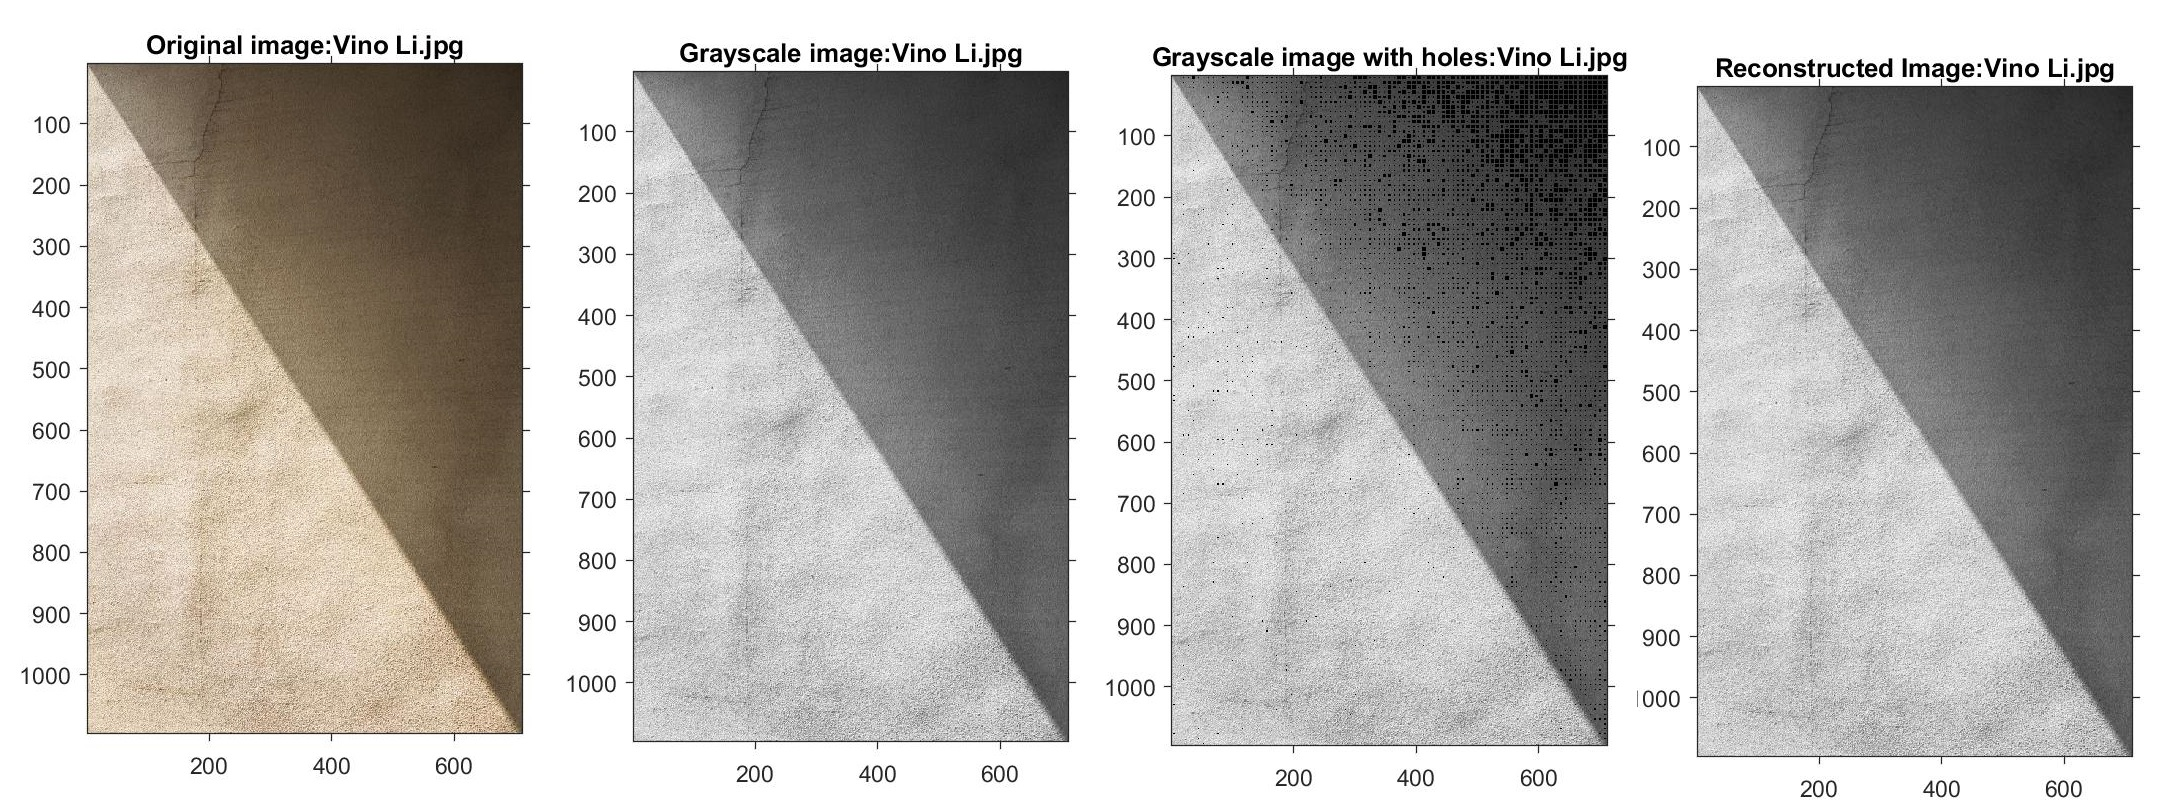
\includegraphics[scale=0.32]{VinoLi.jpg}
\caption{Vino Li texture image with 0\% error introduction}
\label{fig:vlt}
\end{figure}
%%

%%
%% SAME IMAGE DIFFERENT SIZES
%%
%% HIGH CONTRAST IMAGES

%% Ananth Pai

\begin{figure}[!ht]
\center 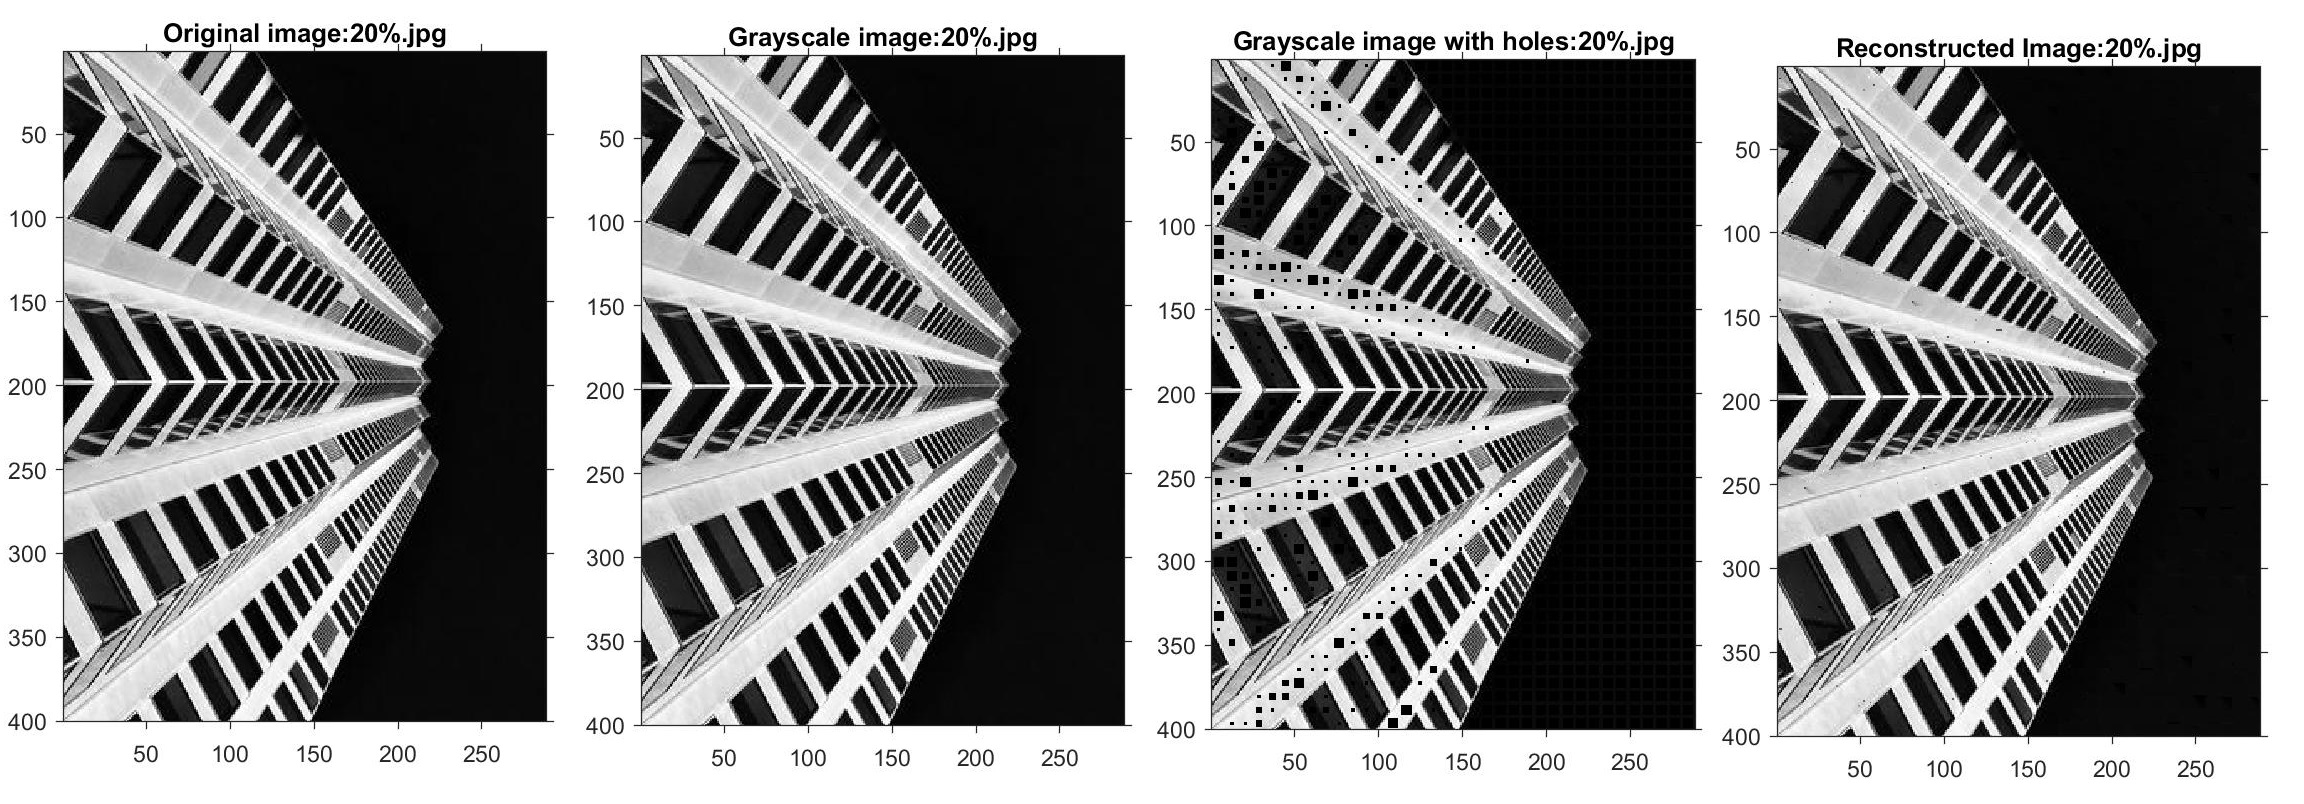
\includegraphics[scale=0.3]{AnanthPai20.jpg}
\caption{Ananth Pai high contrast image at 20\% of the original size with 10\% error introduction}
\label{fig:AnanthPai20}
\end{figure}

\begin{figure}[!ht]
\center 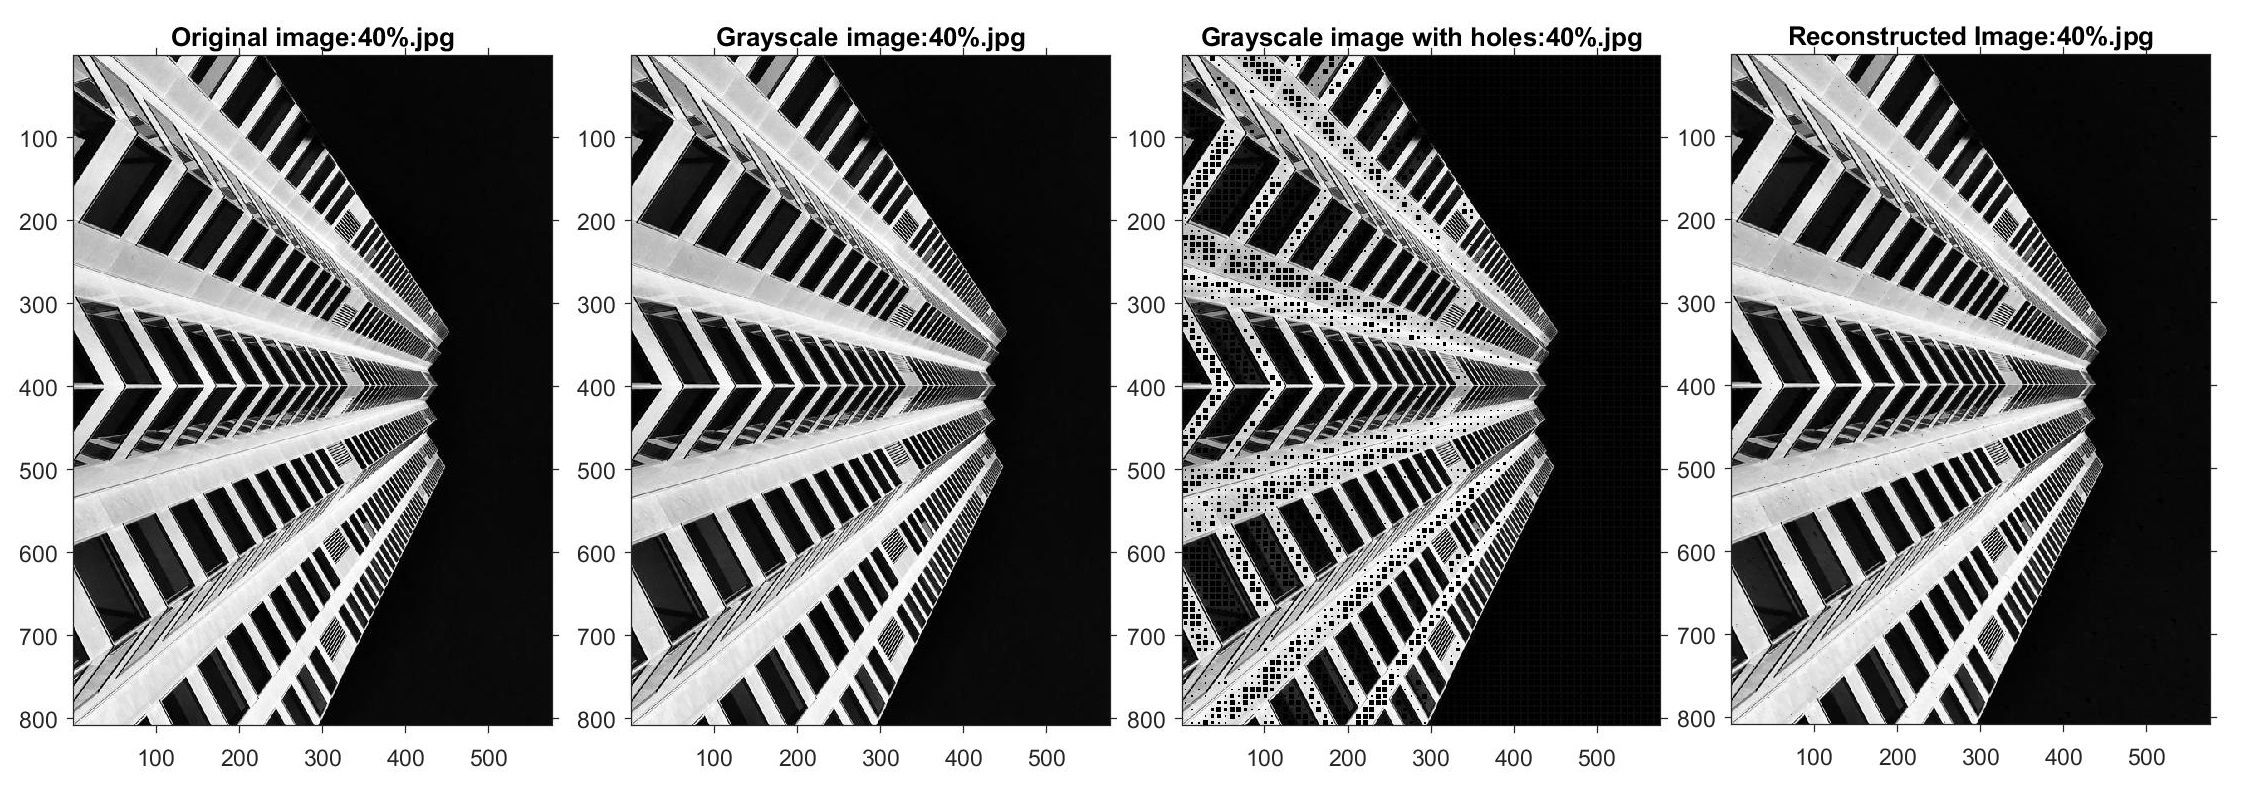
\includegraphics[scale=0.3]{AnanthPai40.jpg}
\caption{Ananth Pai high contrast image at 40\% of the original size with 10\% error introduction}
\label{fig:AnanthPai40}
\end{figure}

\begin{figure}[!ht]
\center 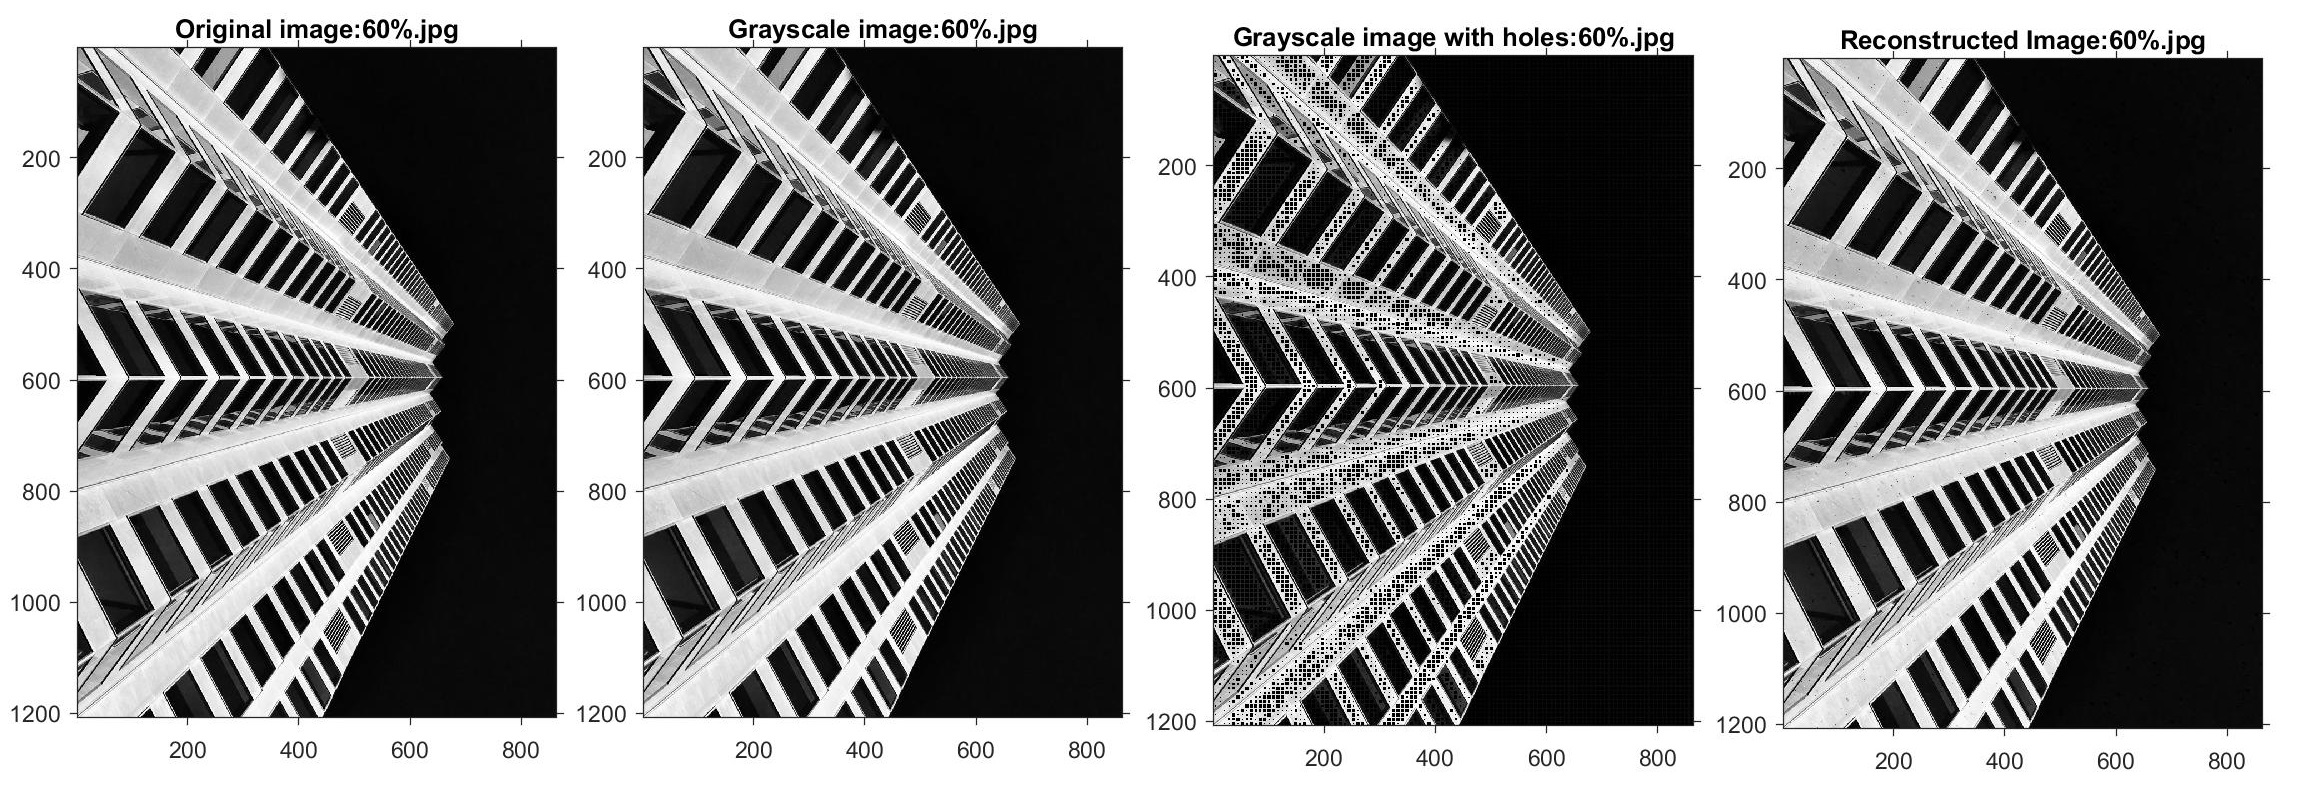
\includegraphics[scale=0.3]{AnanthPai60.jpg}
\caption{Ananth Pai high contrast image at 60\% of the original size with 10\% error introduction}
\label{fig:AnanthPai60}
\end{figure}

\begin{figure}[!ht]
\center 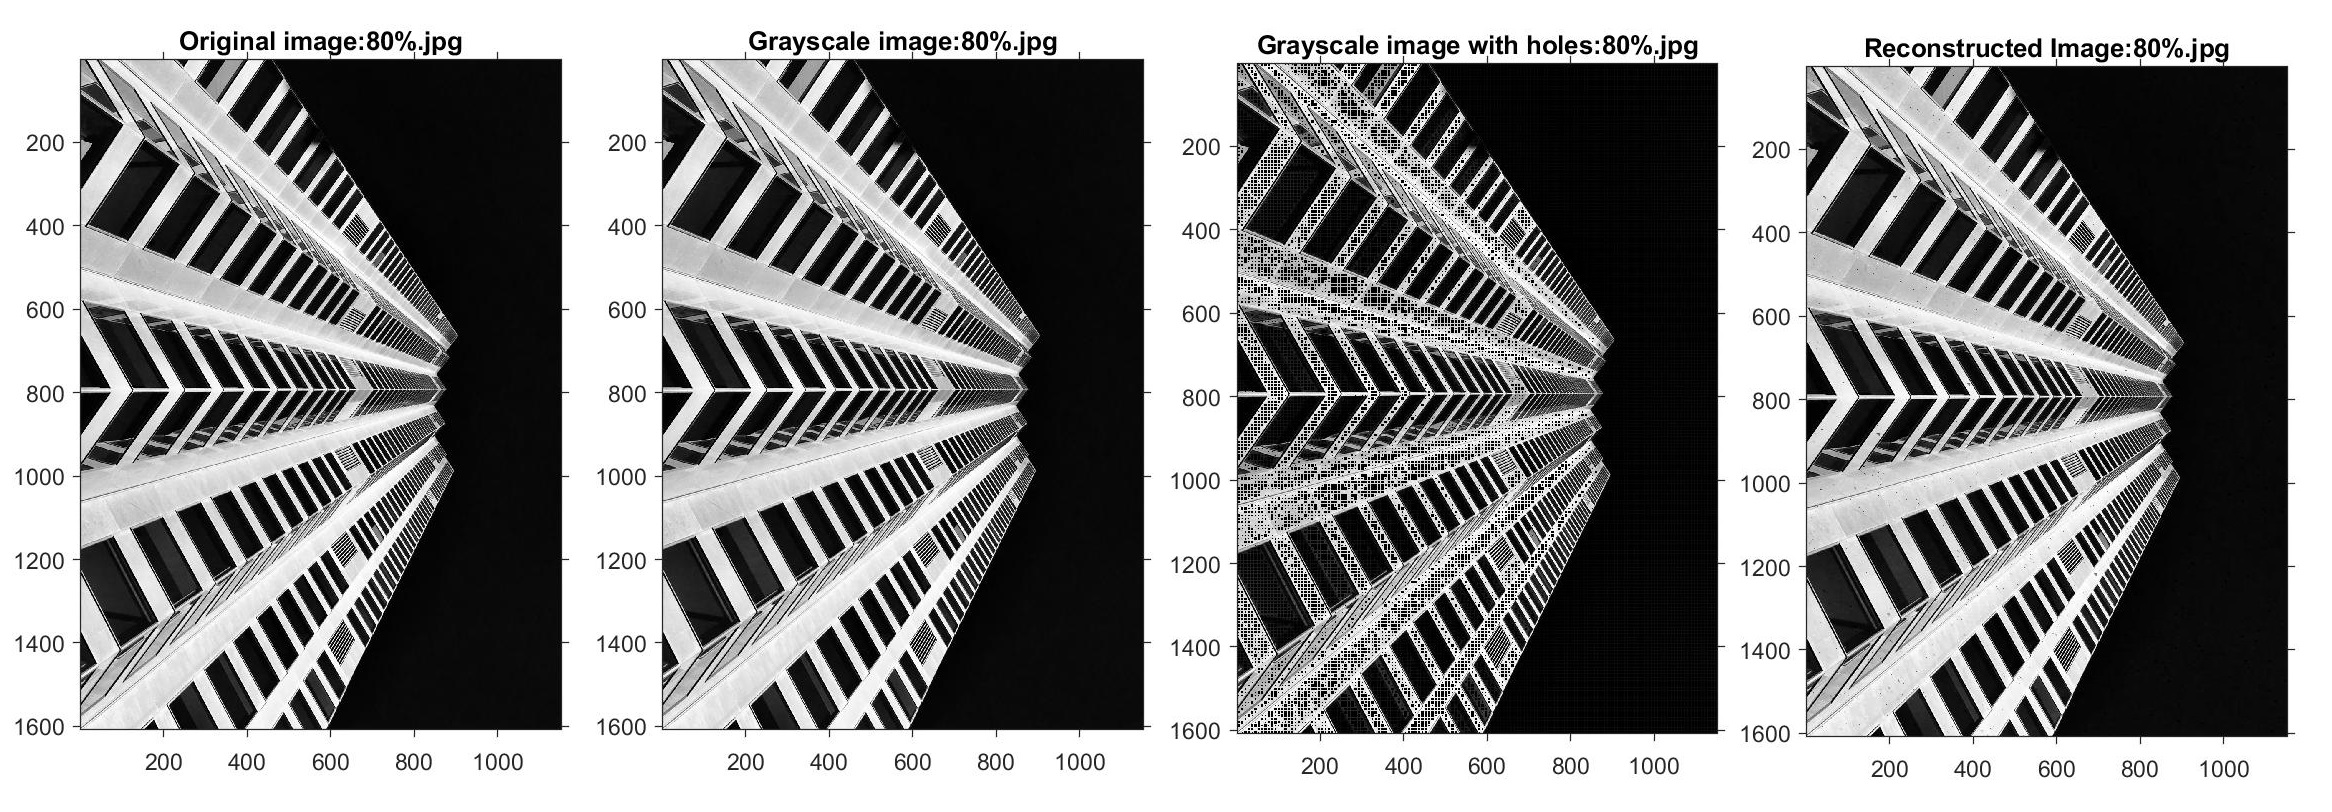
\includegraphics[scale=0.3]{AnanthPai80.jpg}
\caption{Ananth Pai high contrast image at 80\% of the original size with 10\% error introduction}
\label{fig:AnanthPai80}
\end{figure}

\begin{figure}[!ht]
\center 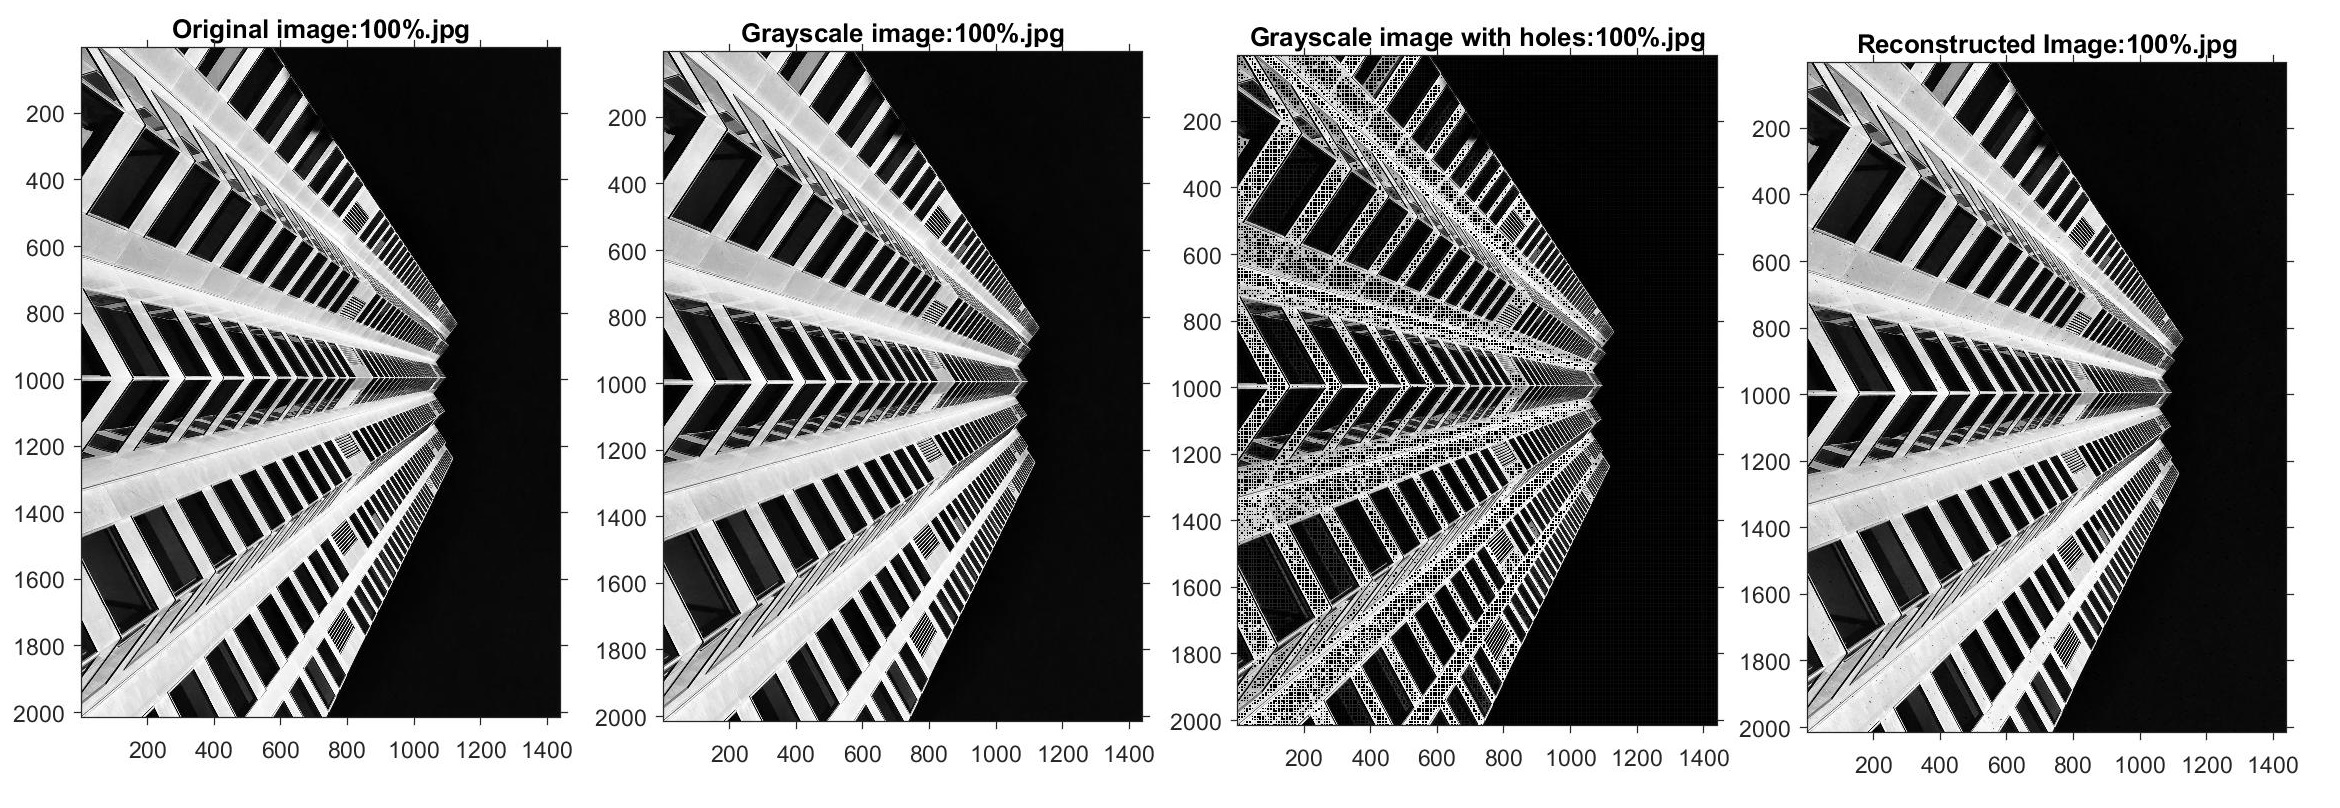
\includegraphics[scale=0.3]{AnanthPai100.jpg}
\caption{Ananth Pai high contrast image at 100\% of the original size with 10\% error introduction}
\label{fig:AnanthPai100}
\end{figure}

%% Ricardo

\begin{figure}[!ht]
\center 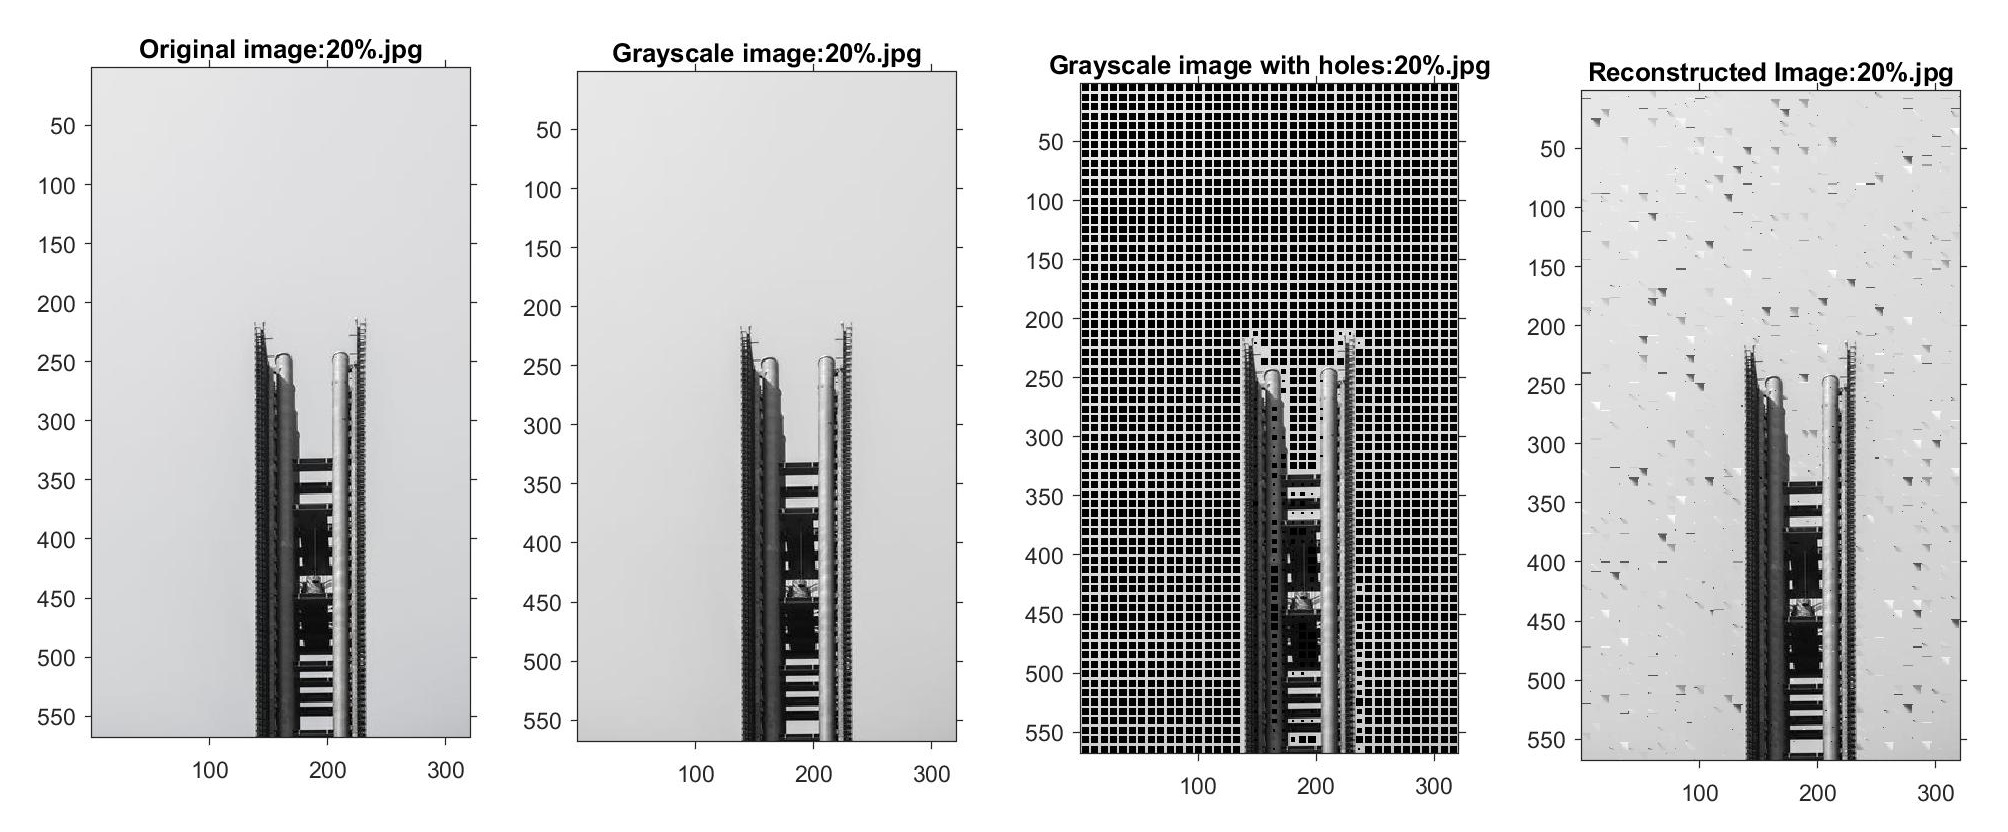
\includegraphics[scale=0.32]{Ricardo20.jpg}
\caption{Ricardo high contrast image at 20\% of the original size with 10\% error introduction}
\label{fig:Ricardo20}
\end{figure}

\begin{figure}[!ht]
\center 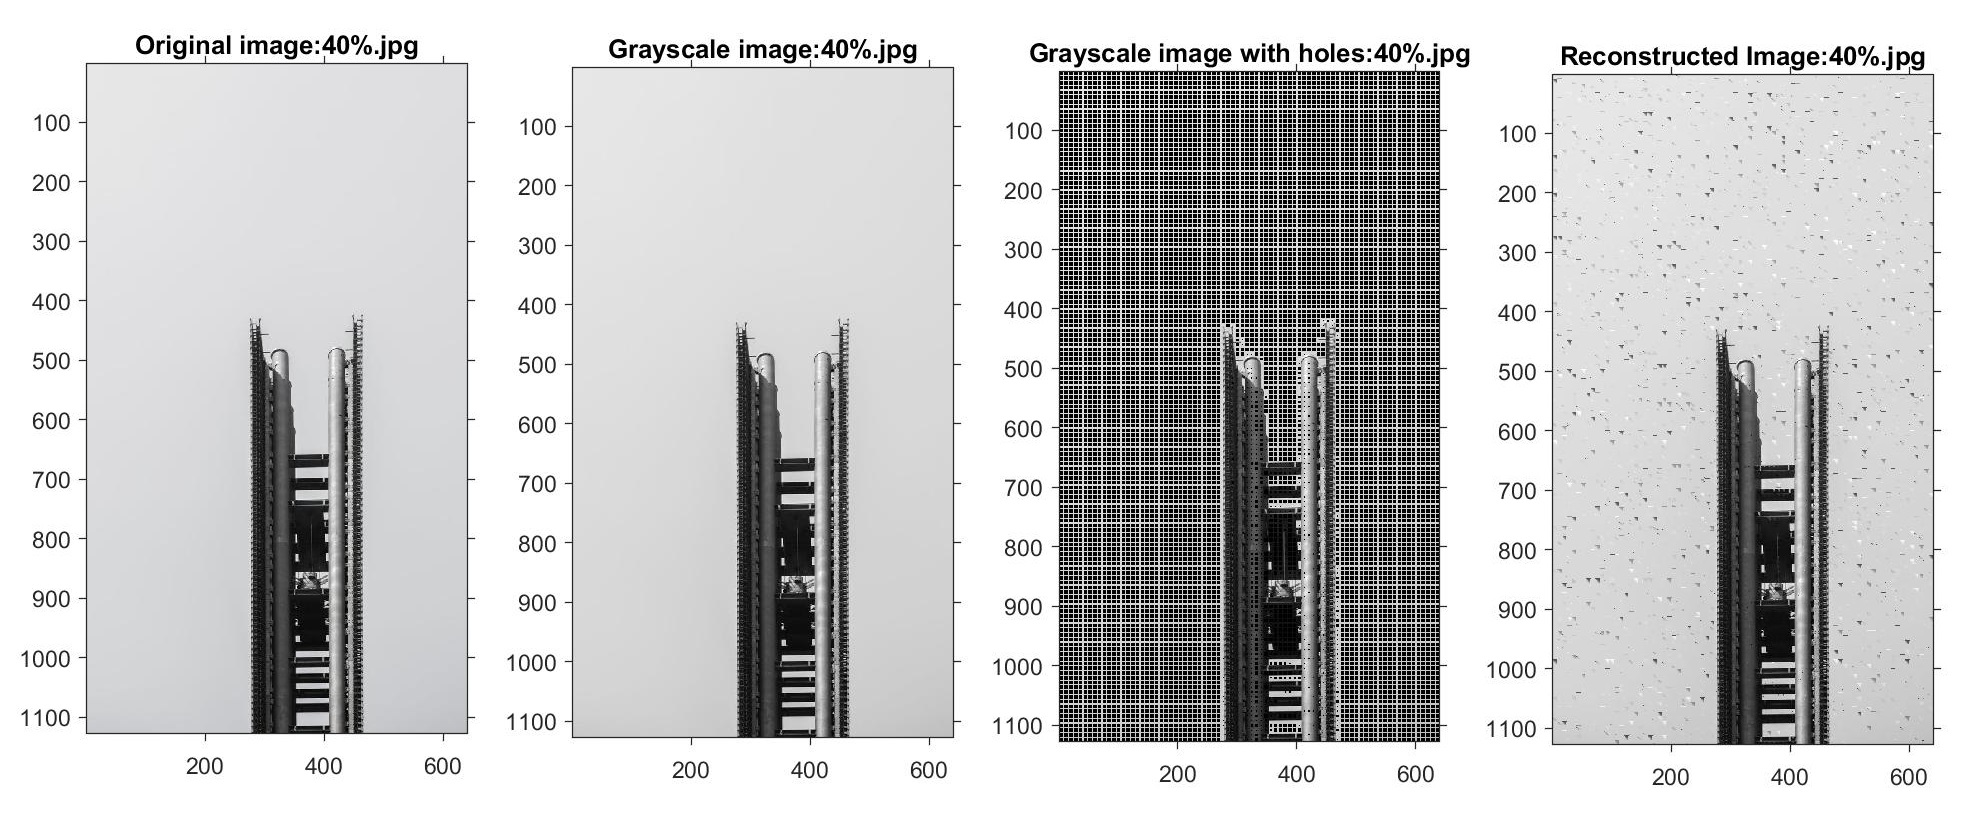
\includegraphics[scale=0.32]{Ricardo40.jpg}
\caption{Ricardo high contrast image at 40\% of the original size with 10\% error introduction}
\label{fig:Ricardo40}
\end{figure}

\begin{figure}[!ht]
\center 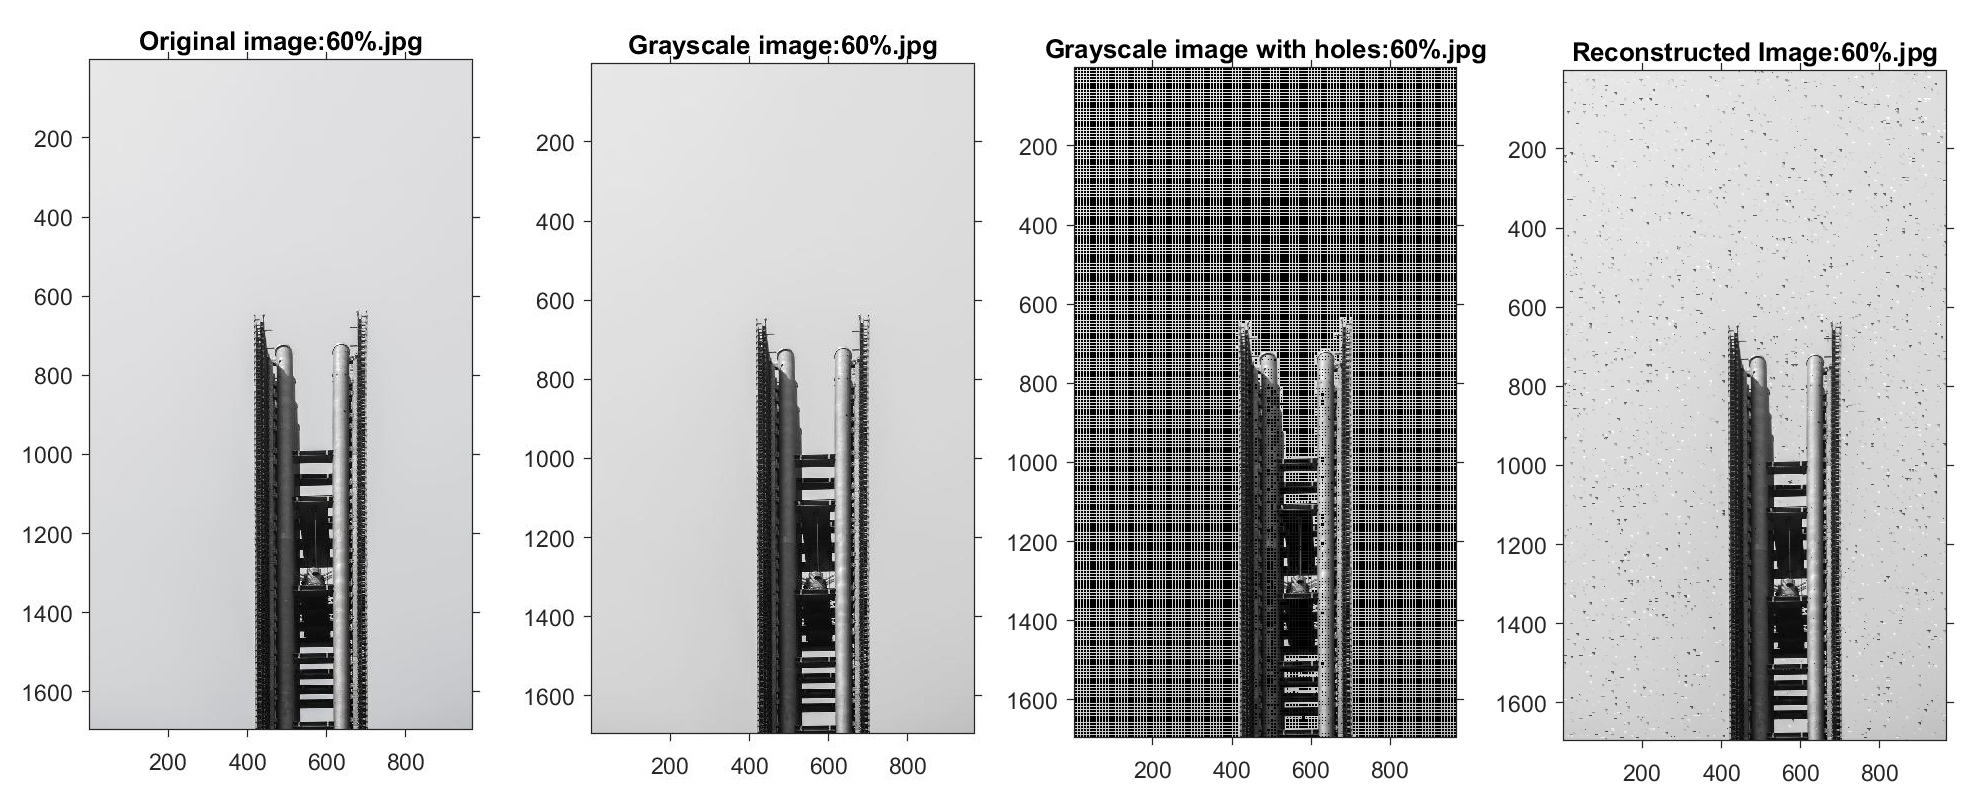
\includegraphics[scale=0.32]{Ricardo60.jpg}
\caption{Ricardo high contrast image at 60\% of the original size with 10\% error introduction}
\label{fig:Ricardo60}
\end{figure}

\begin{figure}[!ht]
\center 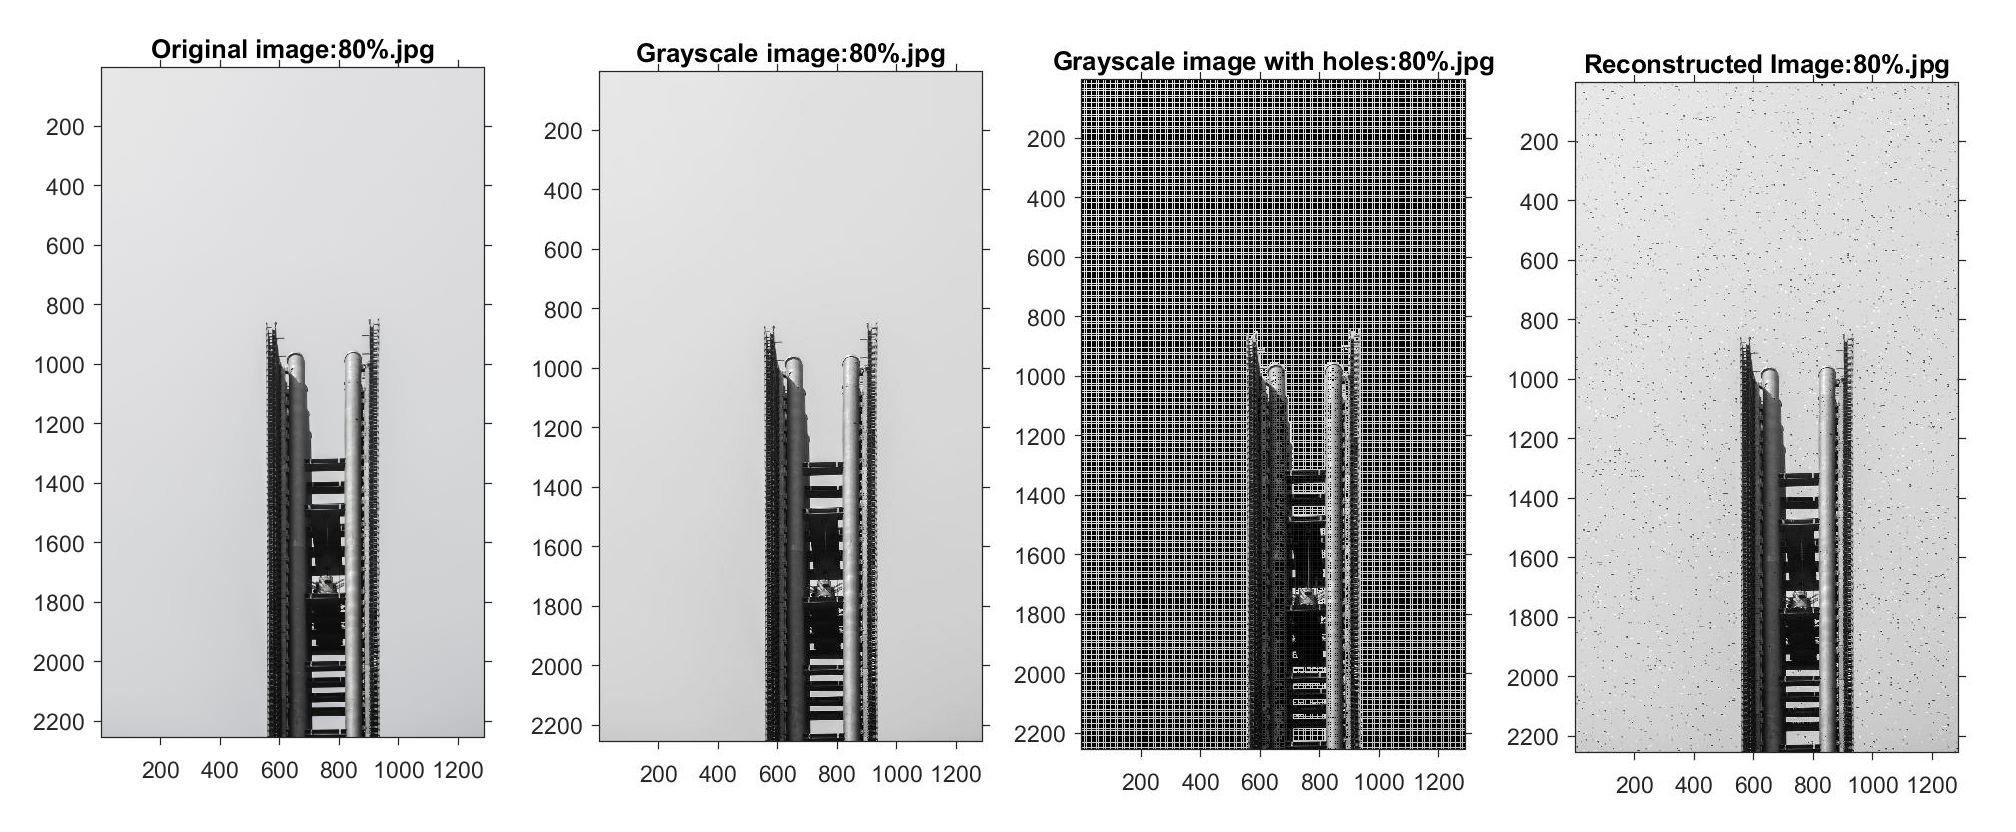
\includegraphics[scale=0.32]{Ricardo80.jpg}
\caption{Ricardo high contrast image at 80\% of the original size with 10\% error introduction}
\label{fig:Ricardo80}
\end{figure}

\begin{figure}[!ht]
\center 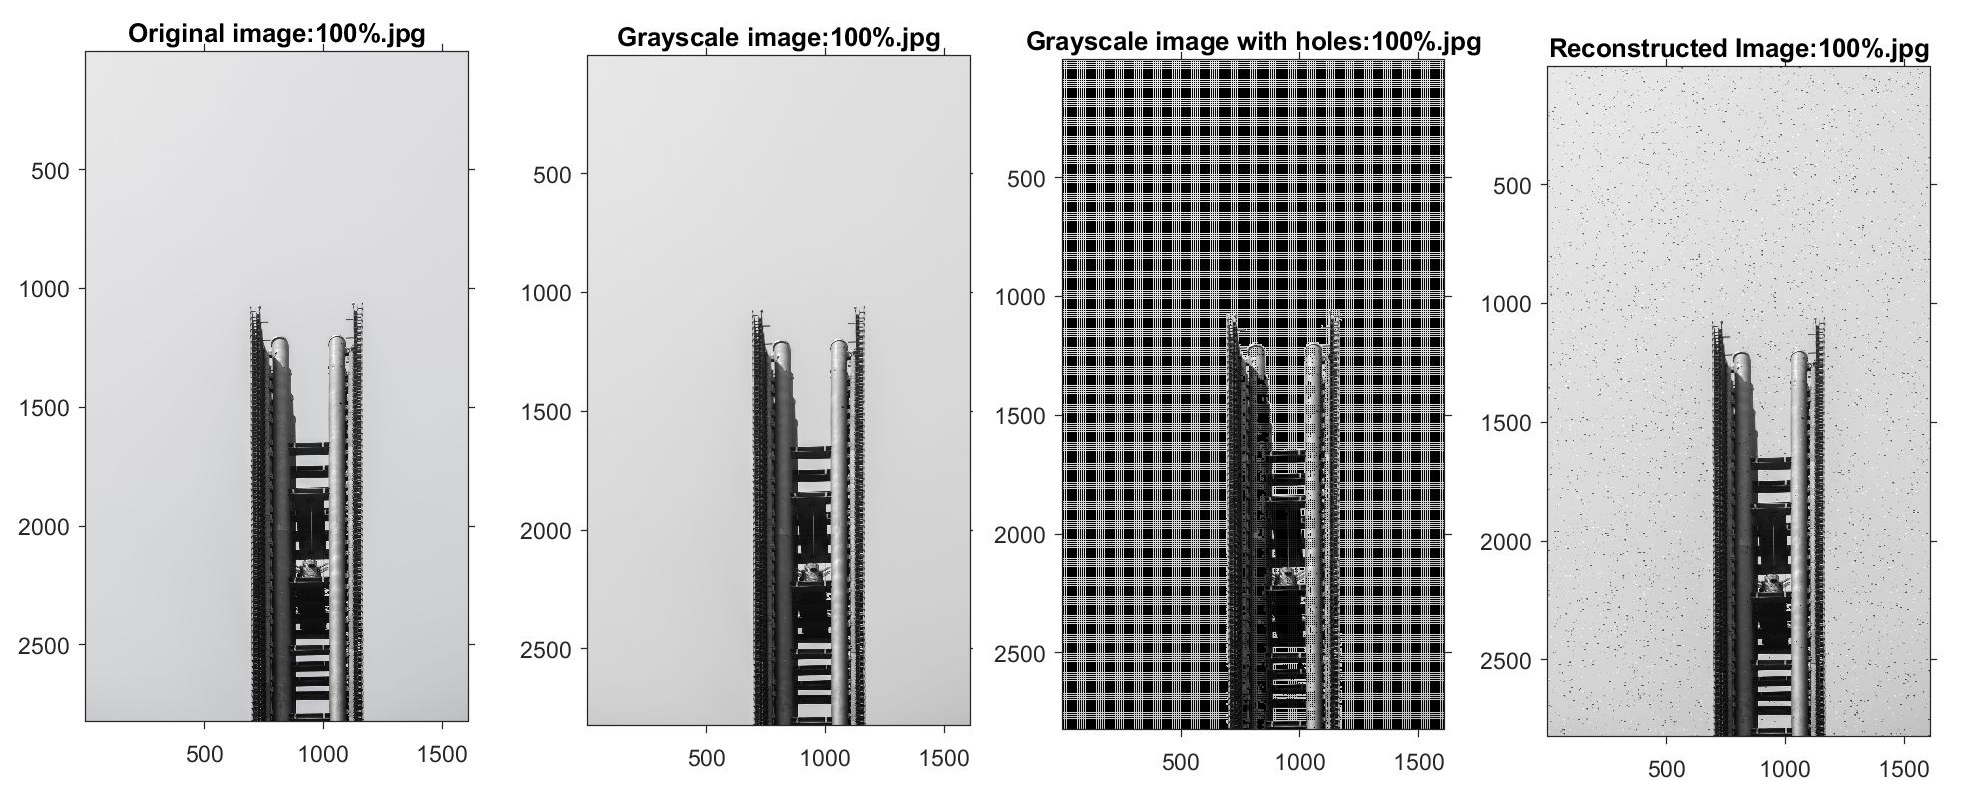
\includegraphics[scale=0.32]{Ricardo100.jpg}
\caption{Ricardo high contrast image at 100\% of the original size with 10\% error introduction}
\label{fig:Ricardo100}
\end{figure}

%% Yerko Lucic

\begin{figure}[!ht]
\center 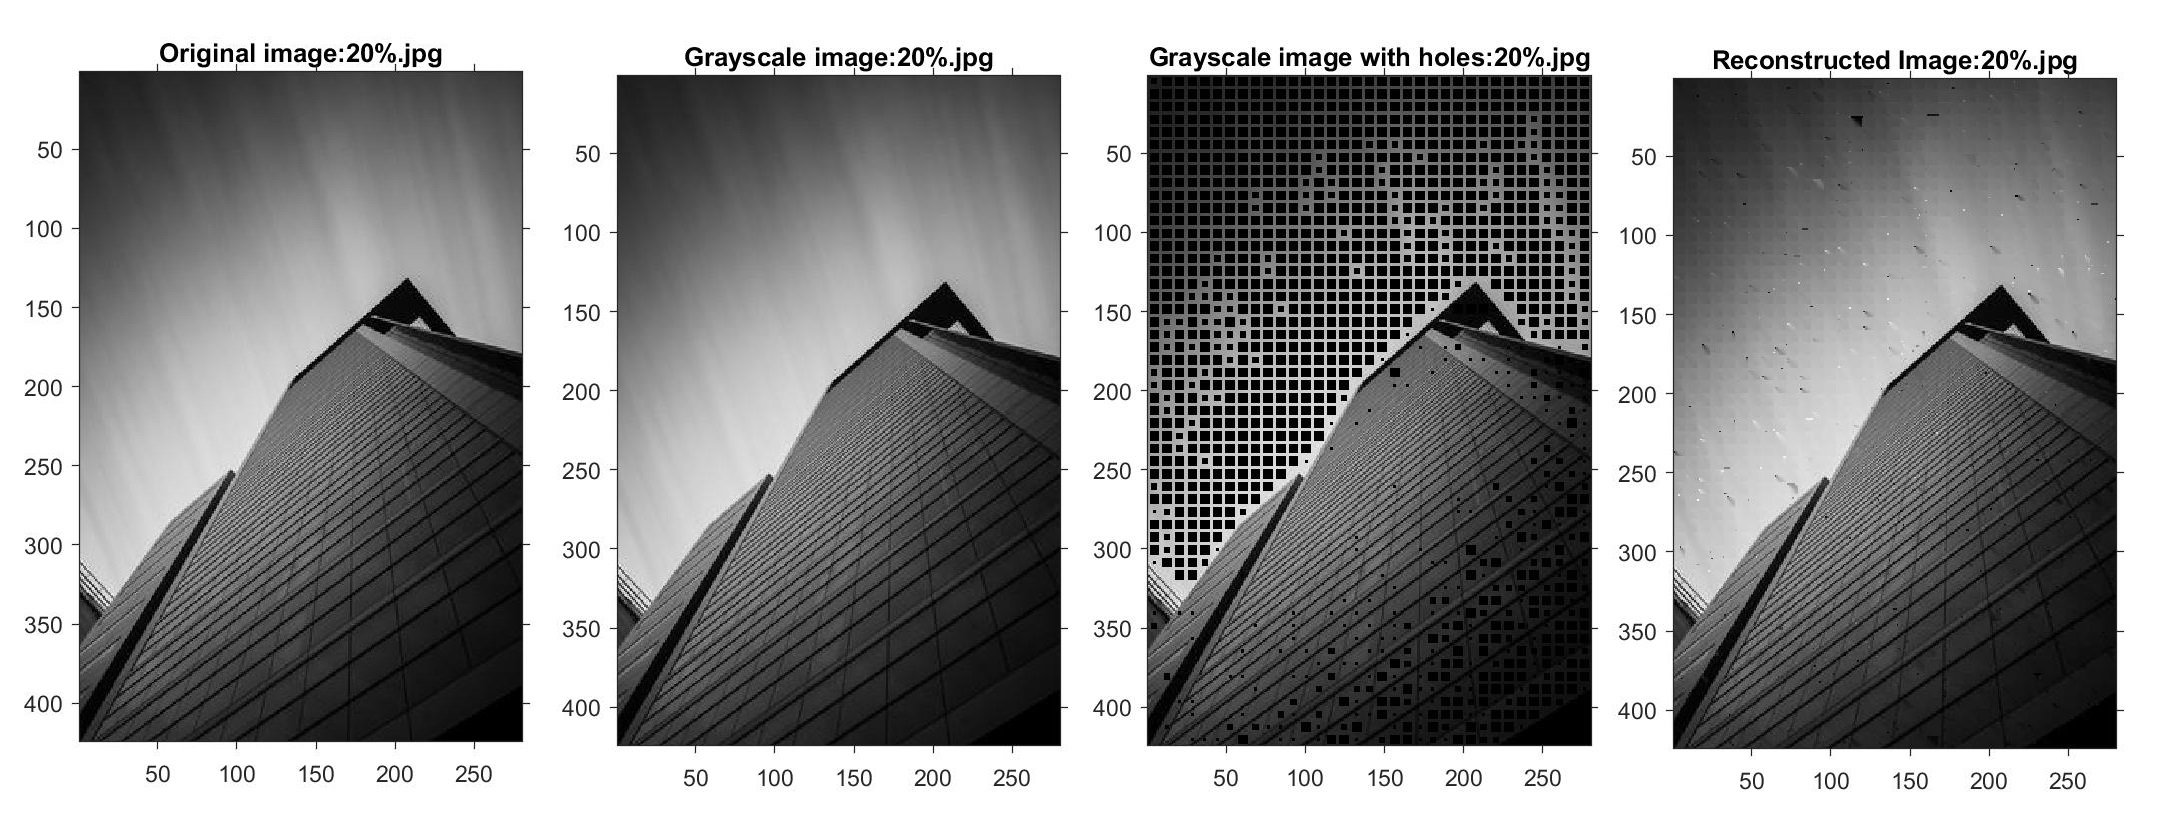
\includegraphics[scale=0.31]{YerkoLucic20.jpg}
\caption{Yerko Lucic high contrast image at 20\% of the original size with 10\% error introduction}
\label{fig:YerkoLucic20}
\end{figure}

\begin{figure}[!ht]
\center 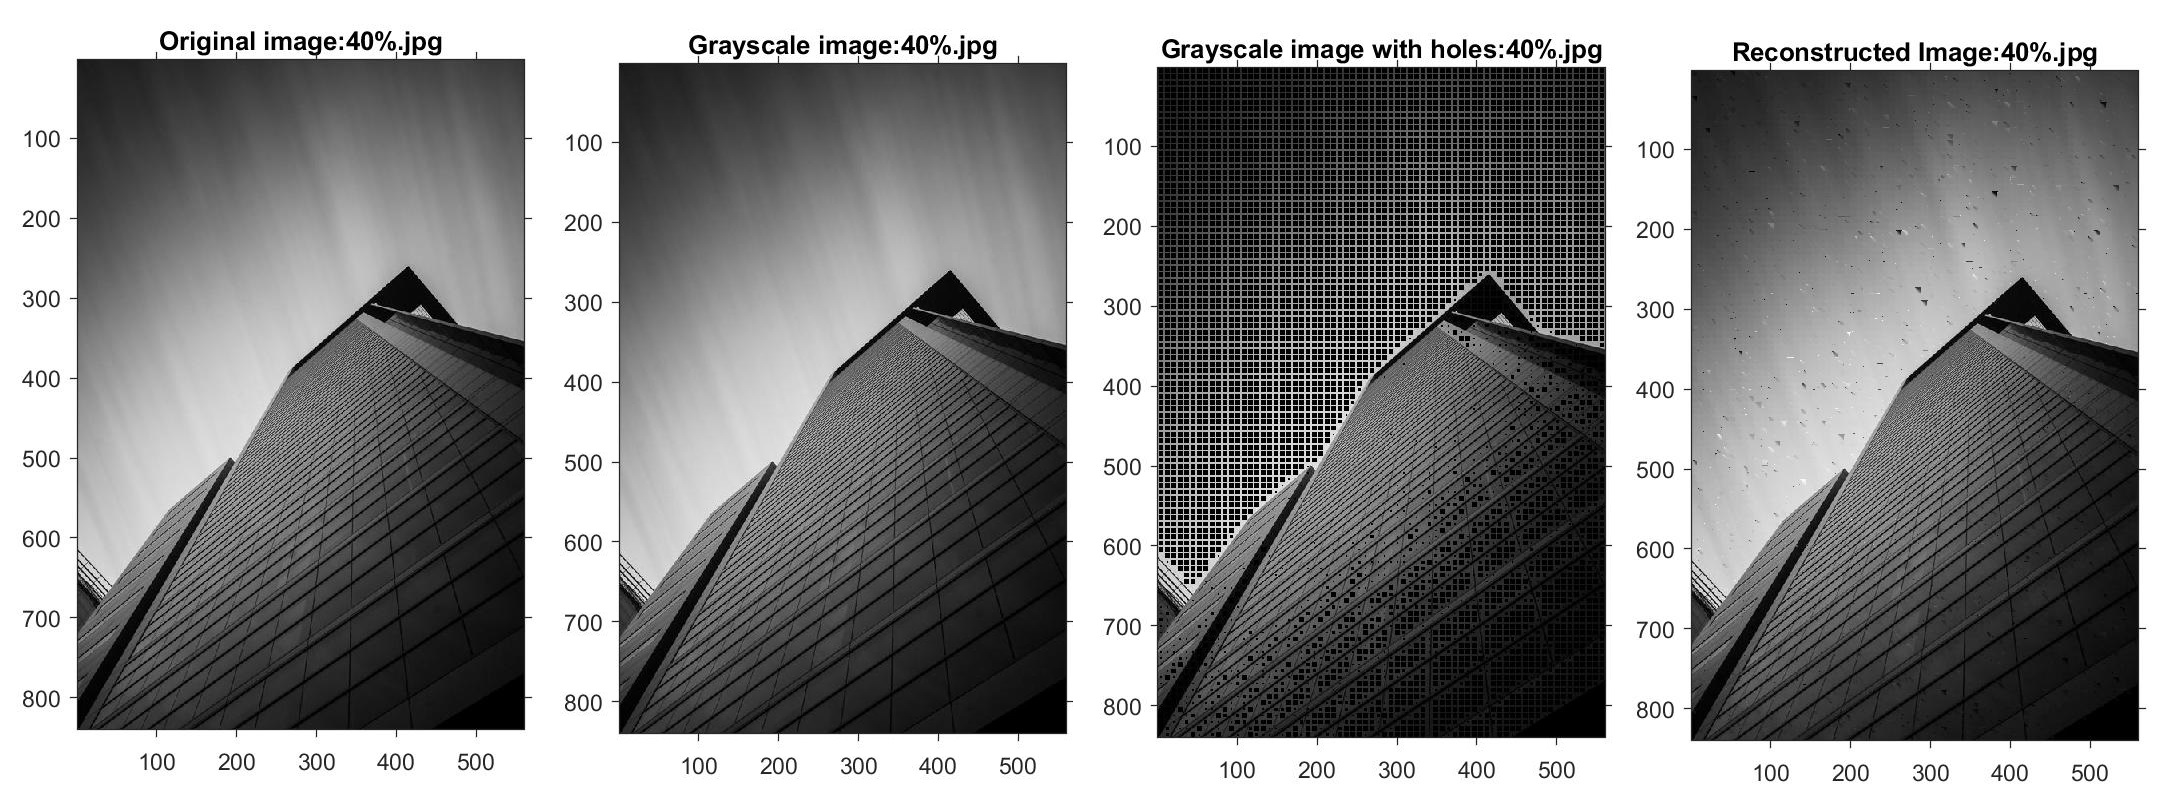
\includegraphics[scale=0.31]{YerkoLucic40.jpg}
\caption{Yerko Lucic high contrast image at 40\% of the original size with 10\% error introduction}
\label{fig:YerkoLucic40}
\end{figure}

\begin{figure}[!ht]
\center 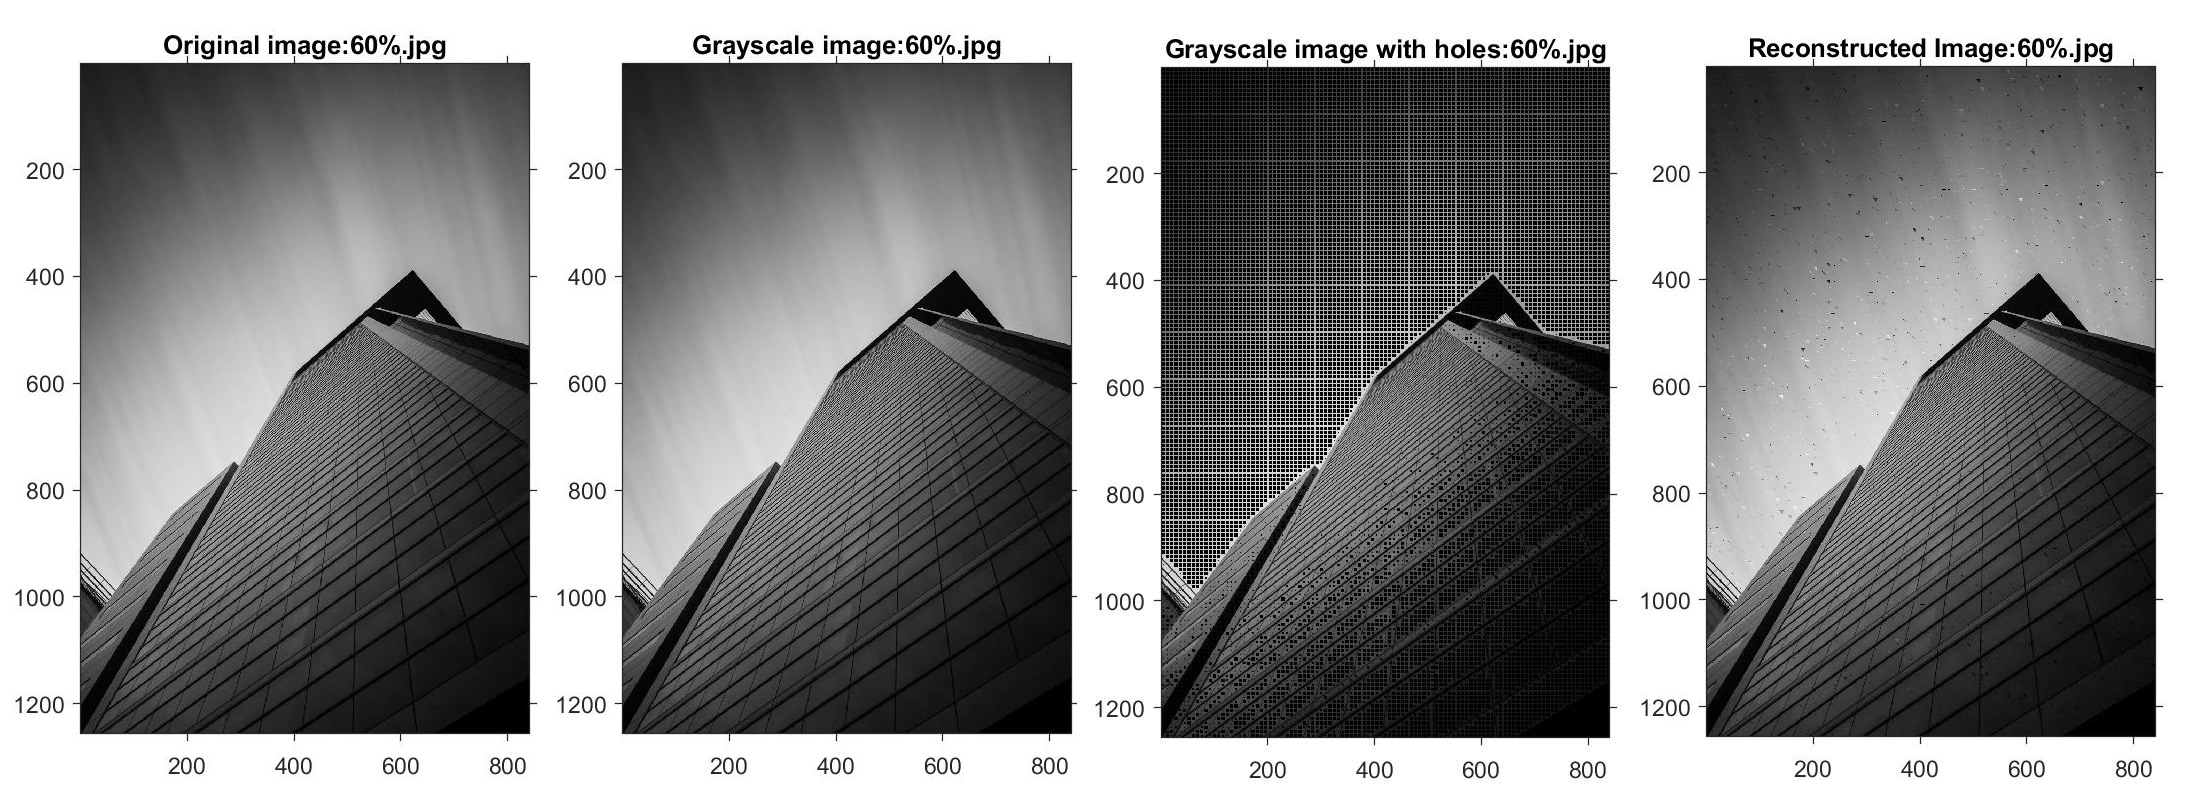
\includegraphics[scale=0.31]{YerkoLucic60.jpg}
\caption{Yerko Lucic high contrast image at 60\% of the original size with 10\% error introduction}
\label{fig:YerkoLucic60}
\end{figure}

\begin{figure}[!ht]
\center 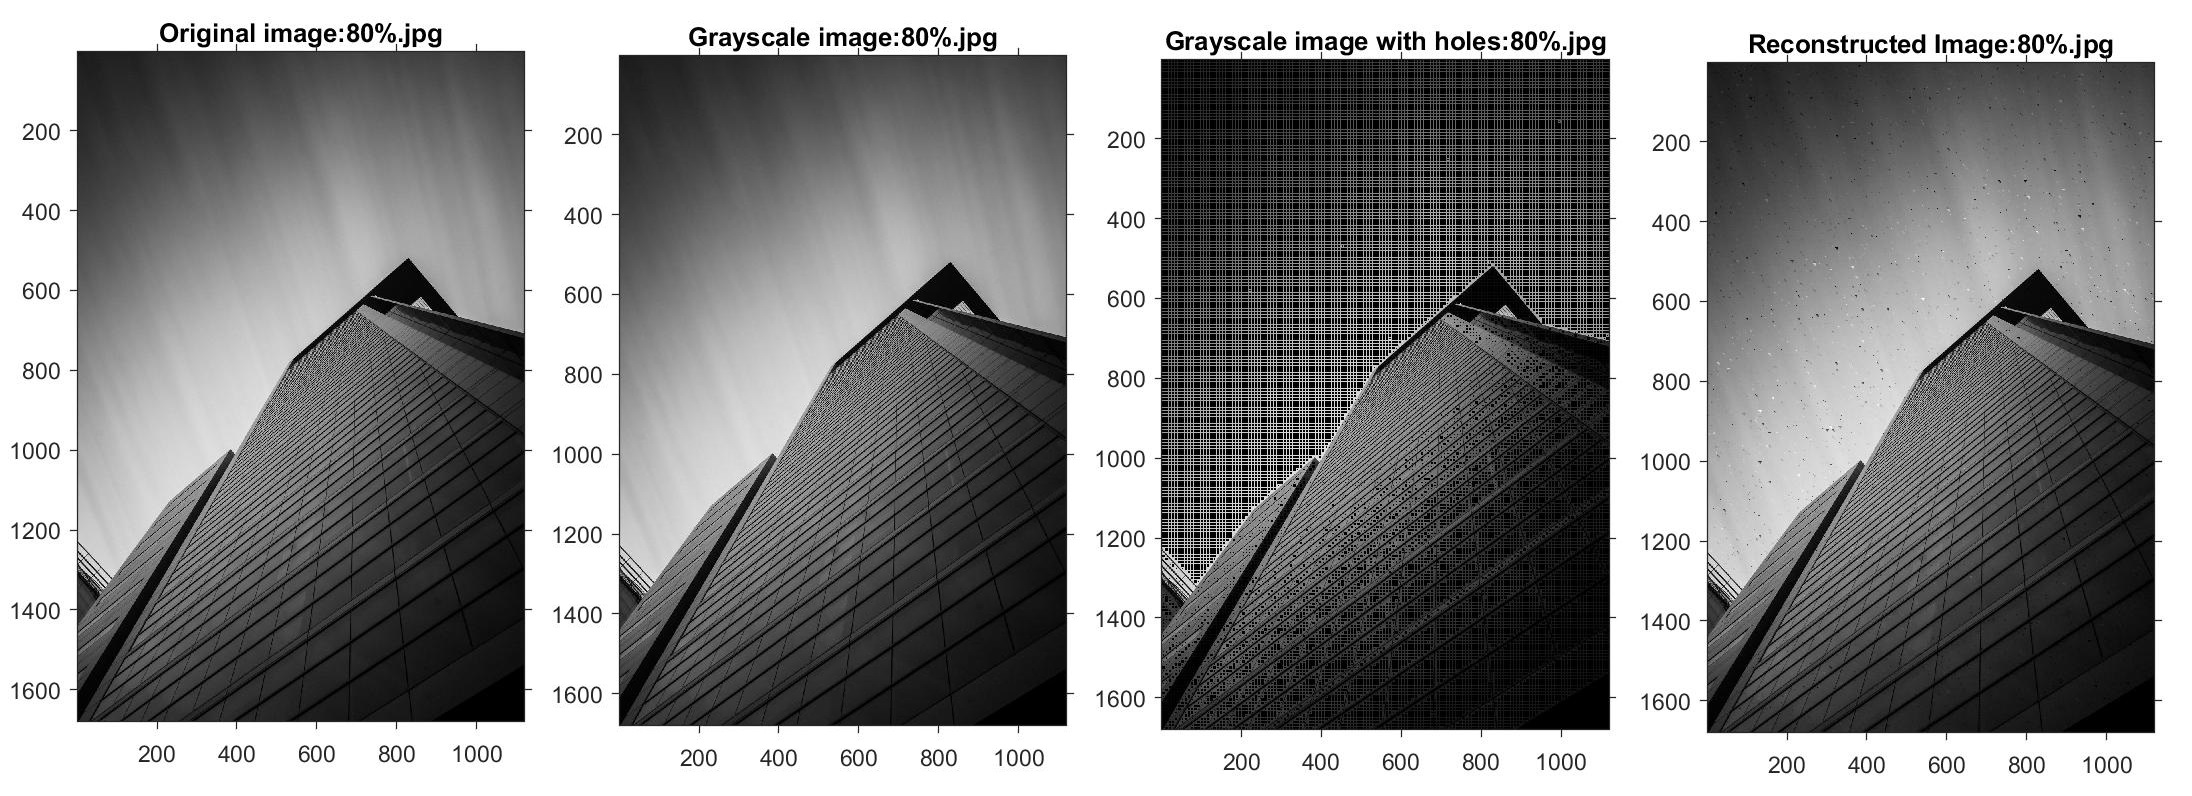
\includegraphics[scale=0.31]{YerkoLucic80.jpg}
\caption{Yerko Lucic high contrast image at 80\% of the original size with 10\% error introduction}
\label{fig:YerkoLucic80}
\end{figure}

\begin{figure}[!ht]
\center 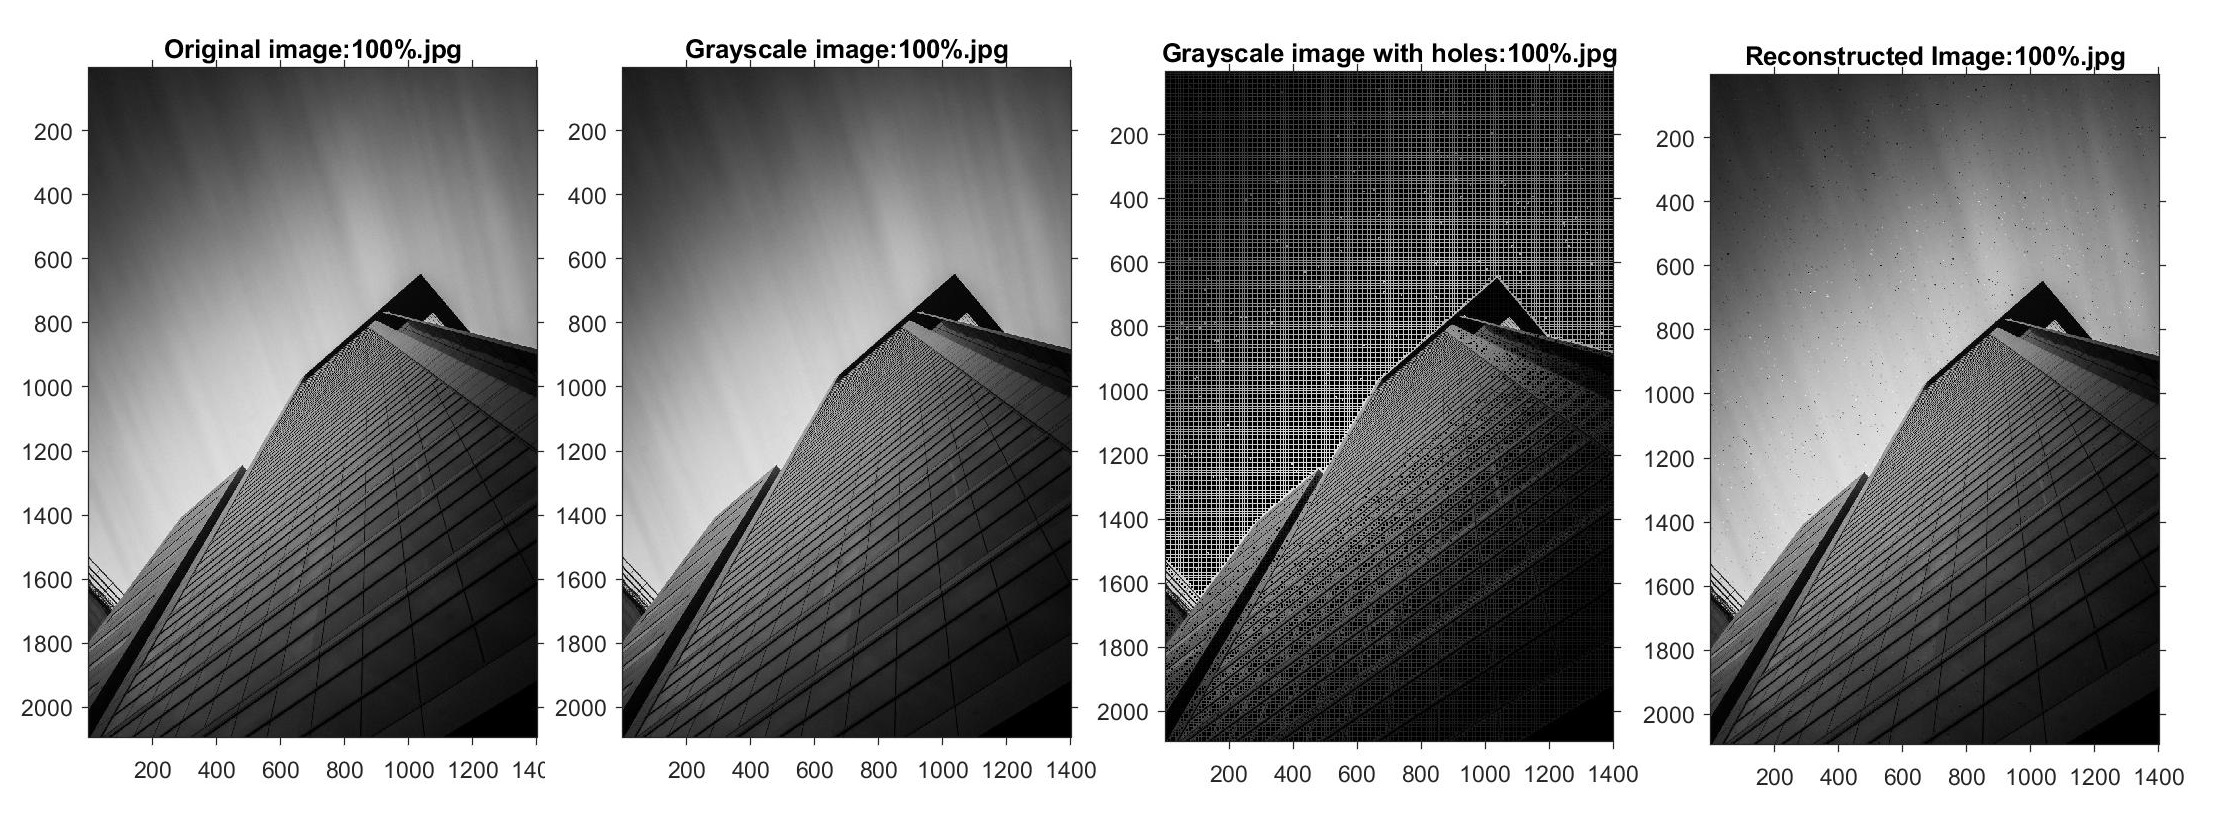
\includegraphics[scale=0.31]{YerkoLucic100.jpg}
\caption{Yerko Lucic high contrast image at 100\% of the original size with 10\% error introduction}
\label{fig:YerkoLucic100}
\end{figure}

%%

%% LANDSCAPE IMAGES
%%
%% Amanda Kerr

\begin{figure}[!ht]
\center 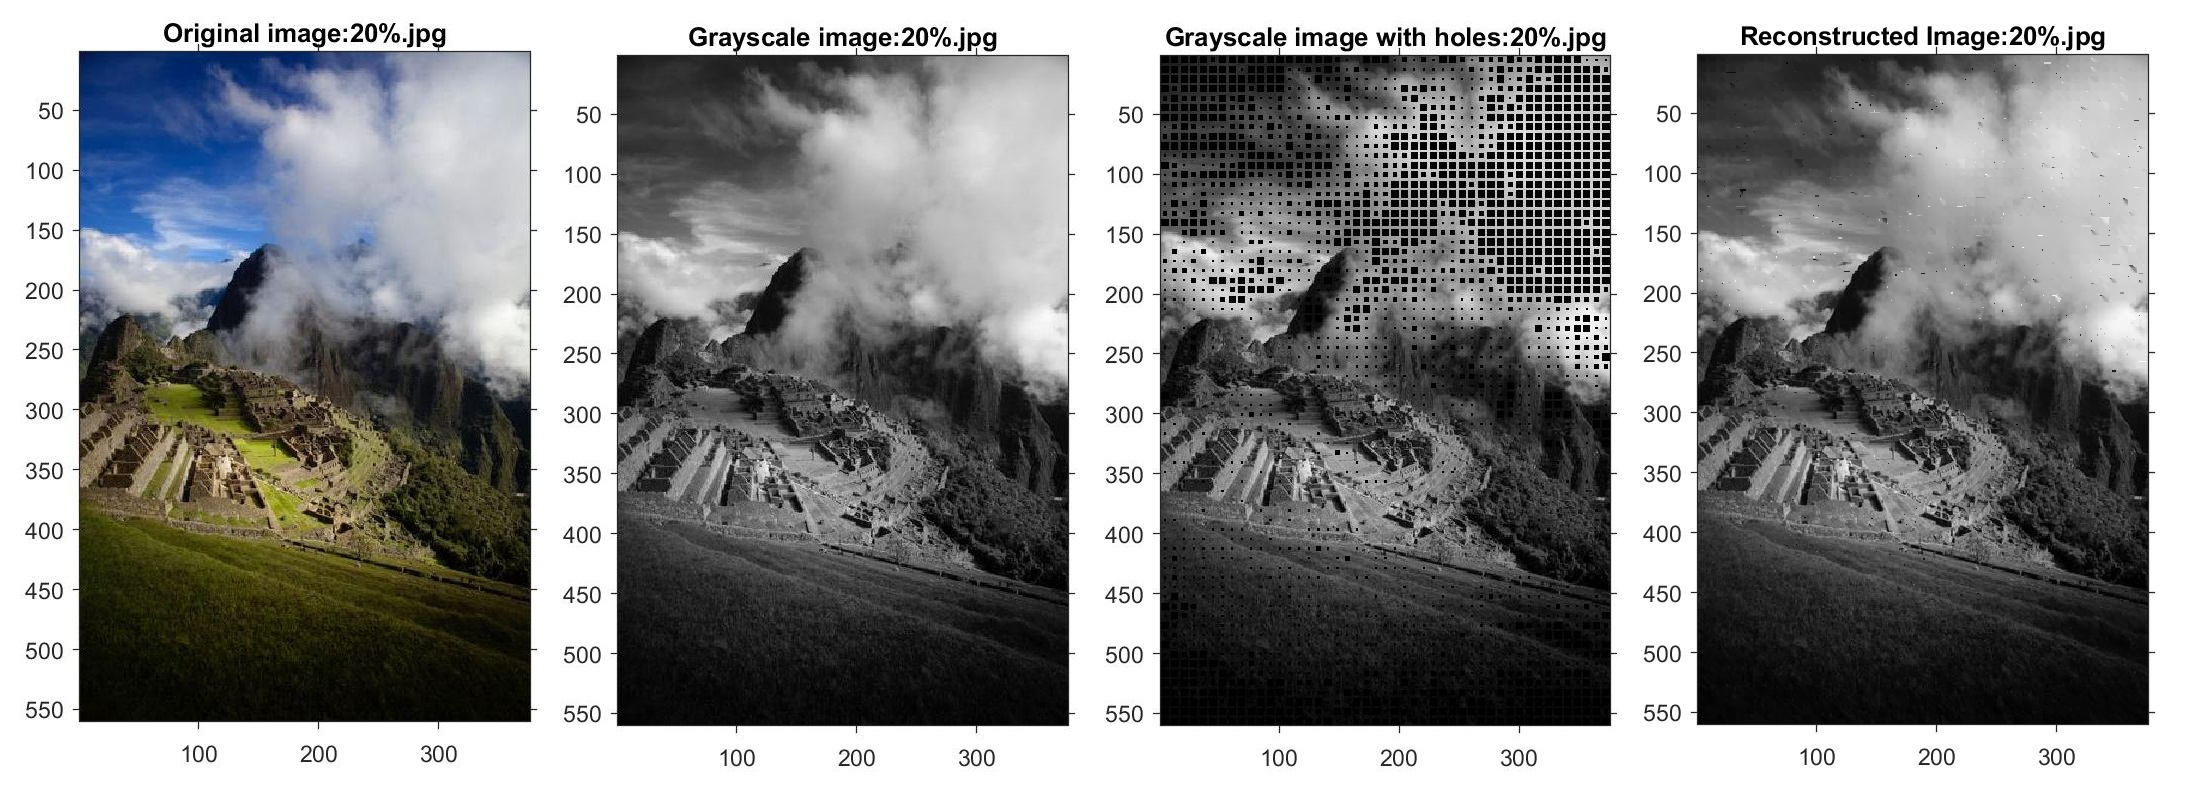
\includegraphics[scale=0.31]{AmandaKerr20.jpg}
\caption{Amanda Kerr landscape image at 20\% of the original size with 10\% error introduction}
\label{fig:AmandaKerr20}
\end{figure}

\begin{figure}[!ht]
\center 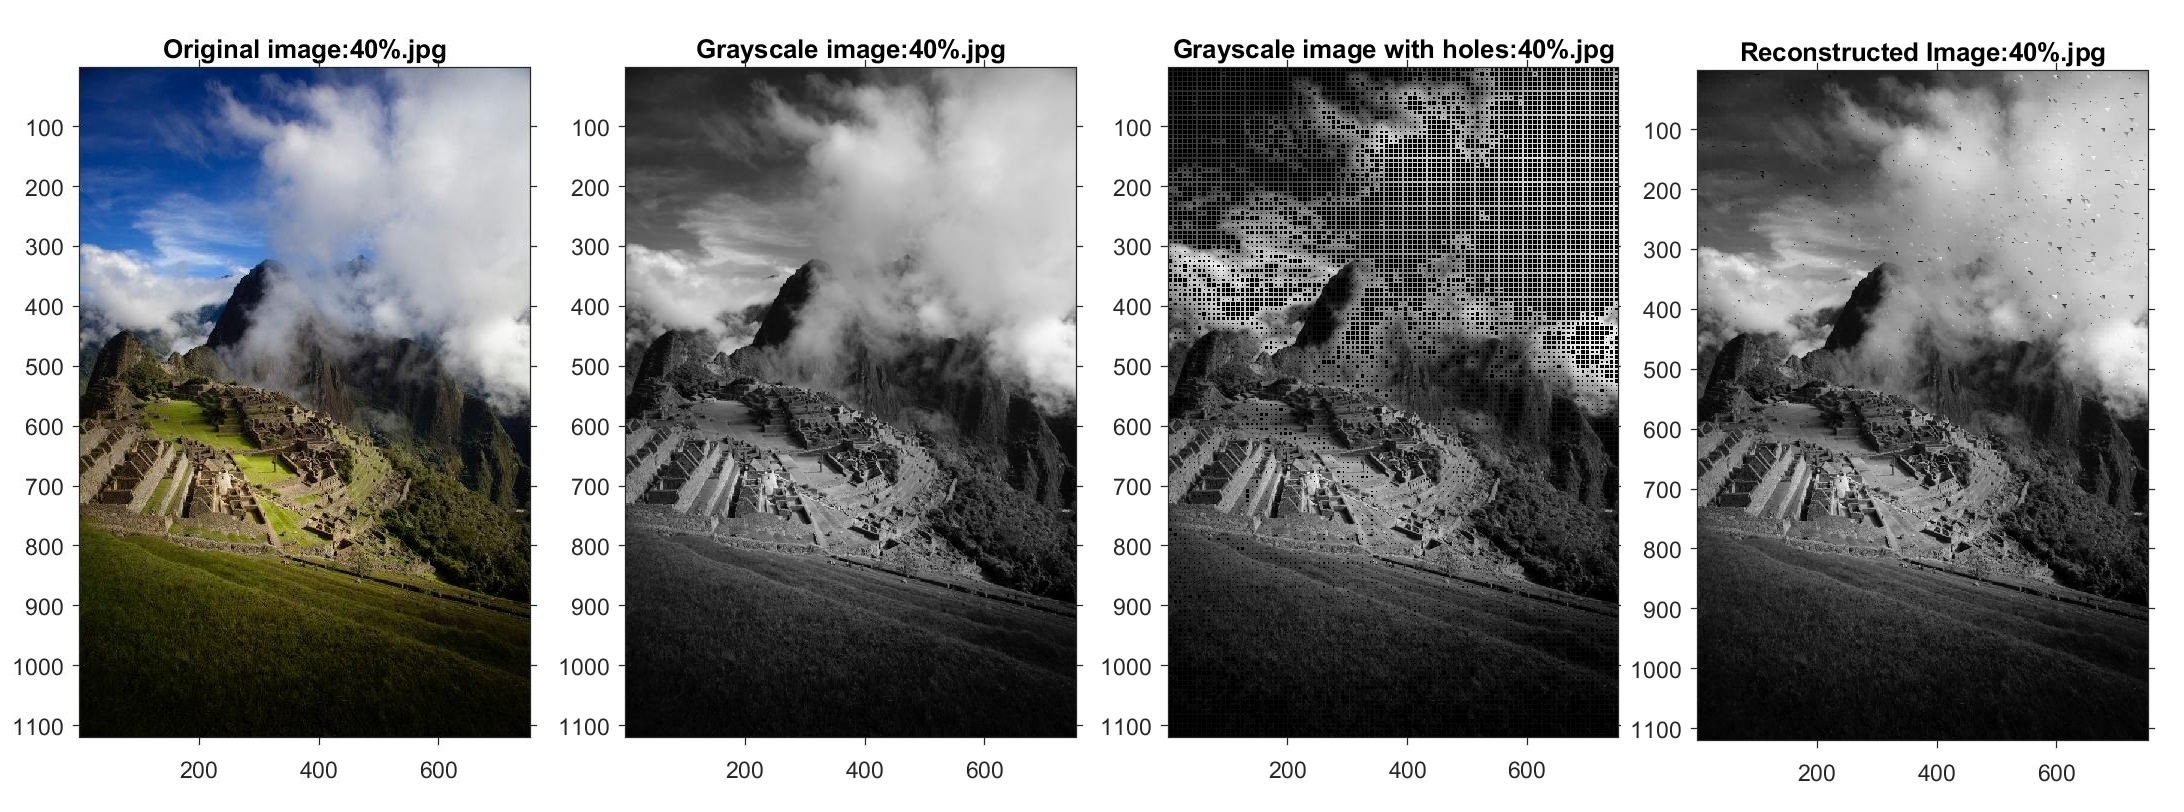
\includegraphics[scale=0.31]{AmandaKerr40.jpg}
\caption{Amanda Kerr landscape image at 40\% of the original size with 10\% error introduction}
\label{fig:AmandaKerr40}
\end{figure}

\begin{figure}[!ht]
\center 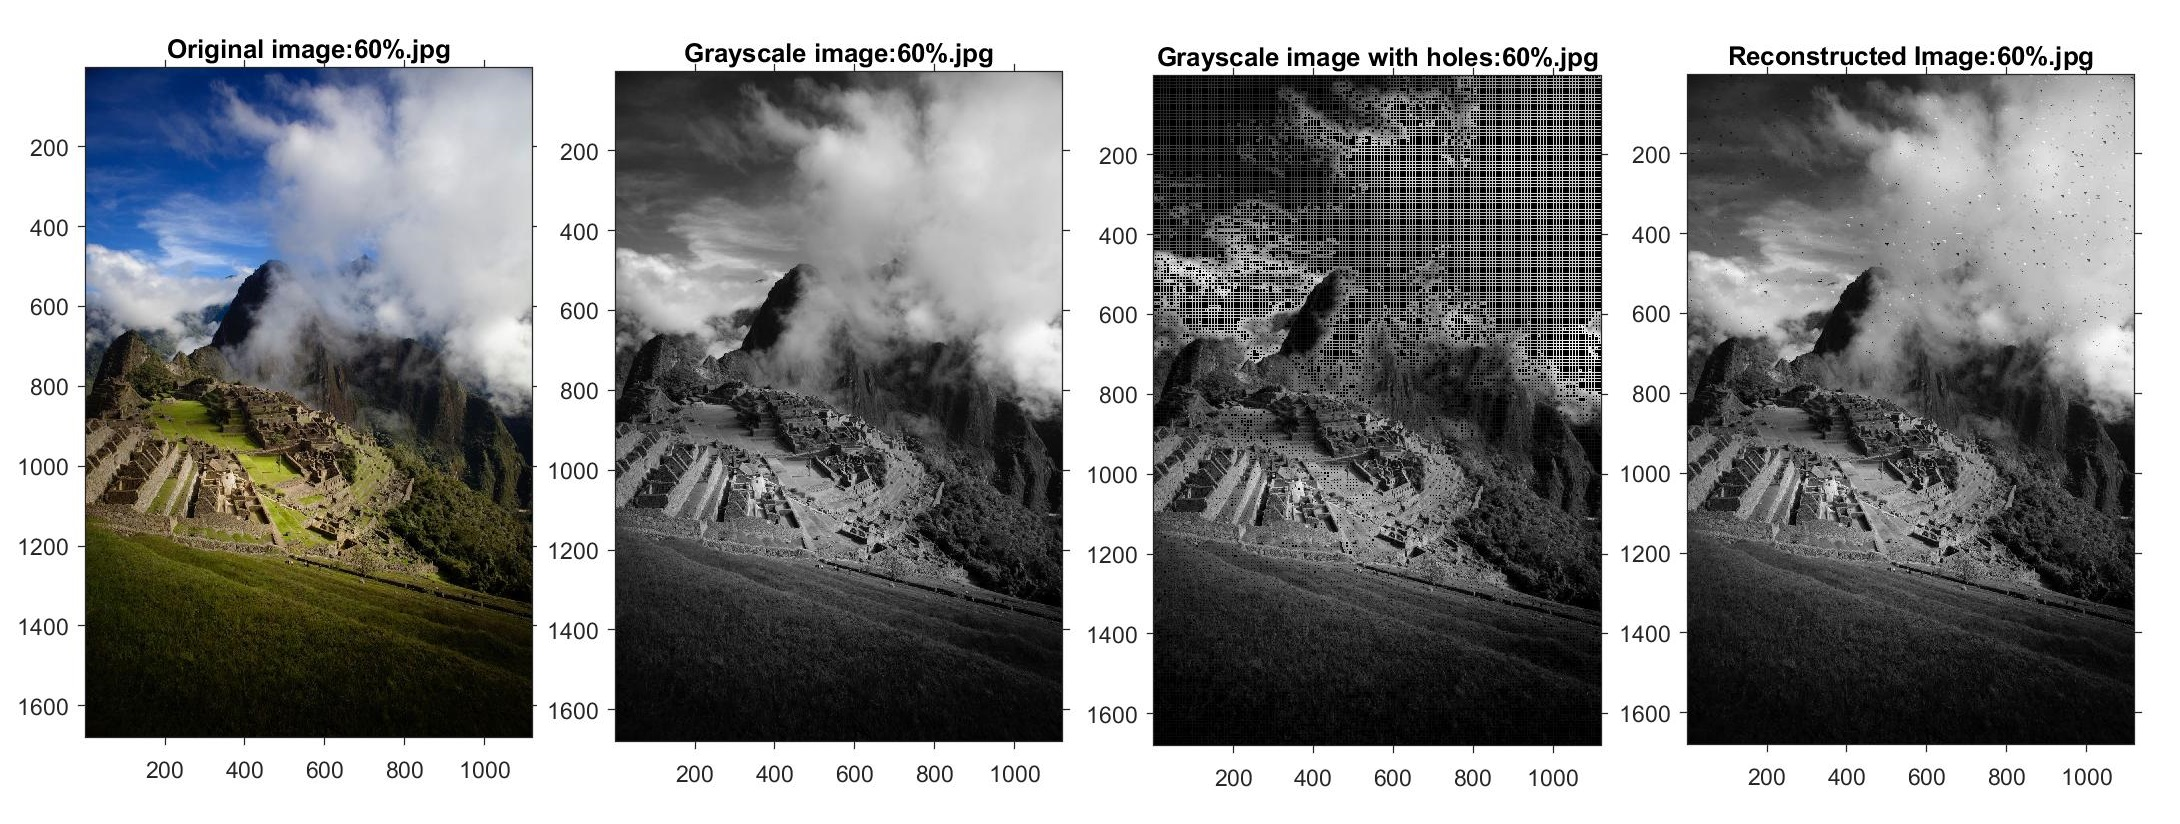
\includegraphics[scale=0.31]{AmandaKerr60.jpg}
\caption{Amanda Kerr landscape image at 60\% of the original size with 10\% error introduction}
\label{fig:AmandaKerr60}
\end{figure}

\begin{figure}[!ht]
\center 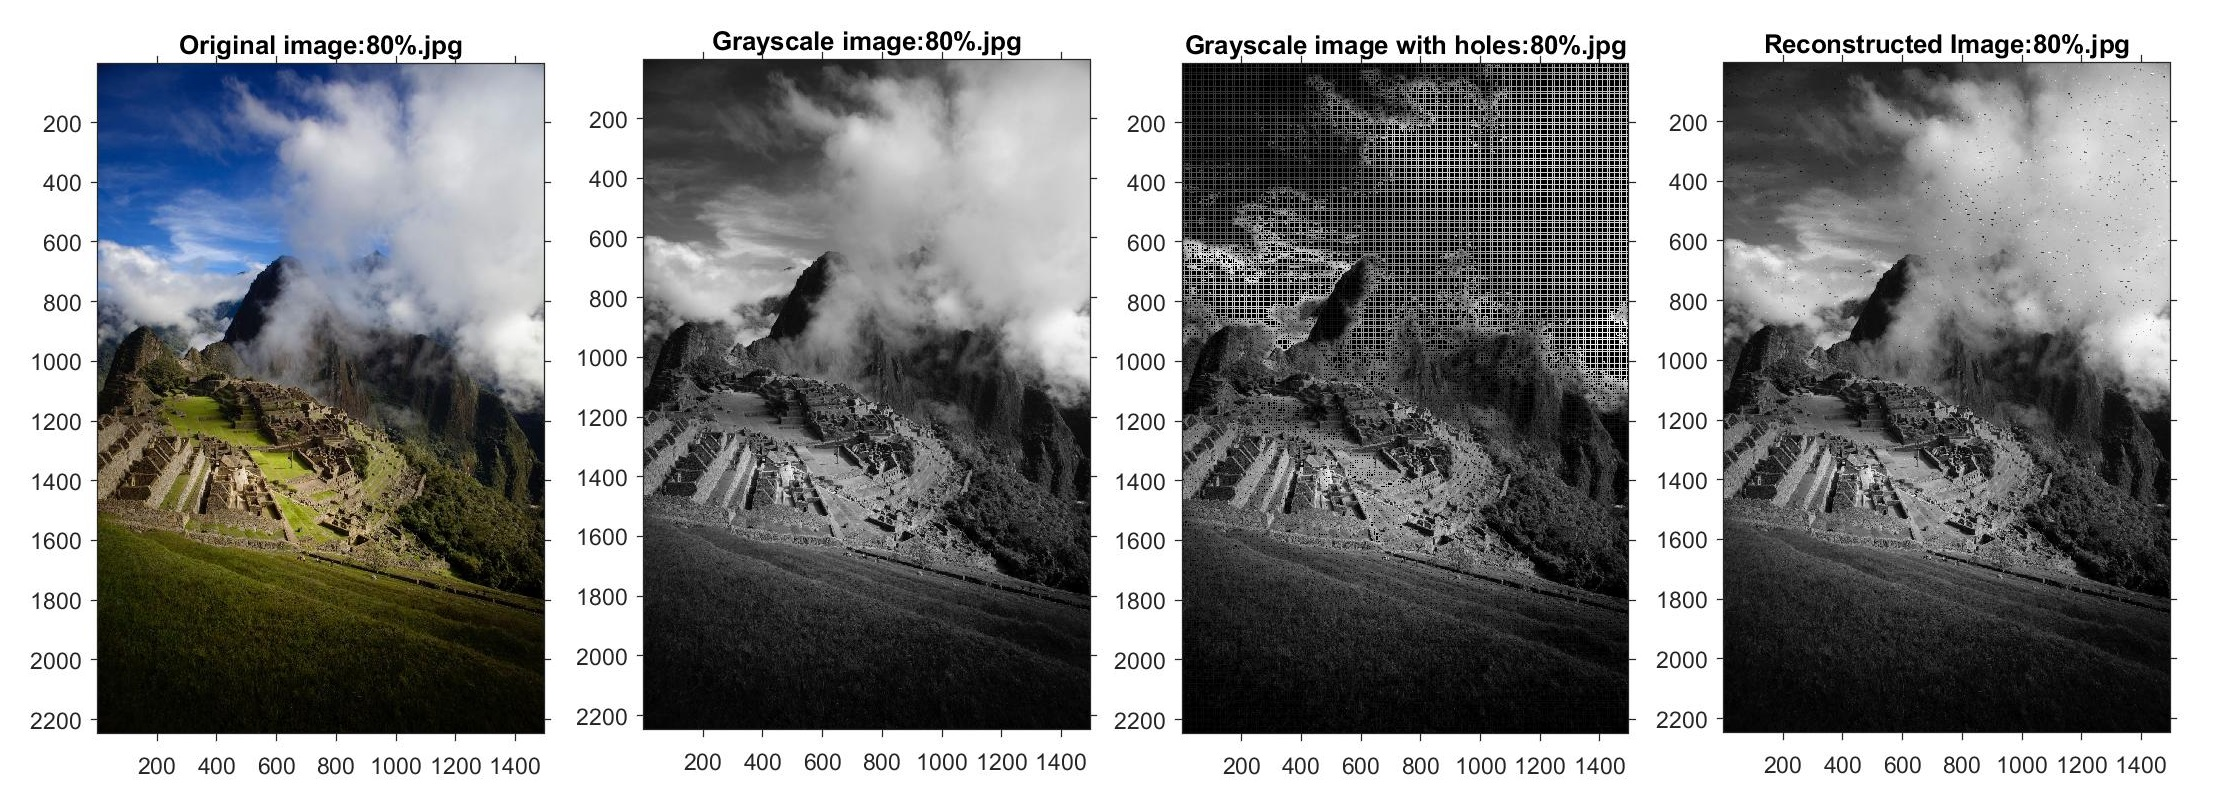
\includegraphics[scale=0.31]{AmandaKerr80.jpg}
\caption{Amanda Kerr landscape image at 80\% of the original size with 10\% error introduction}
\label{fig:AmandaKerr80}
\end{figure}

\begin{figure}[!ht]
\center 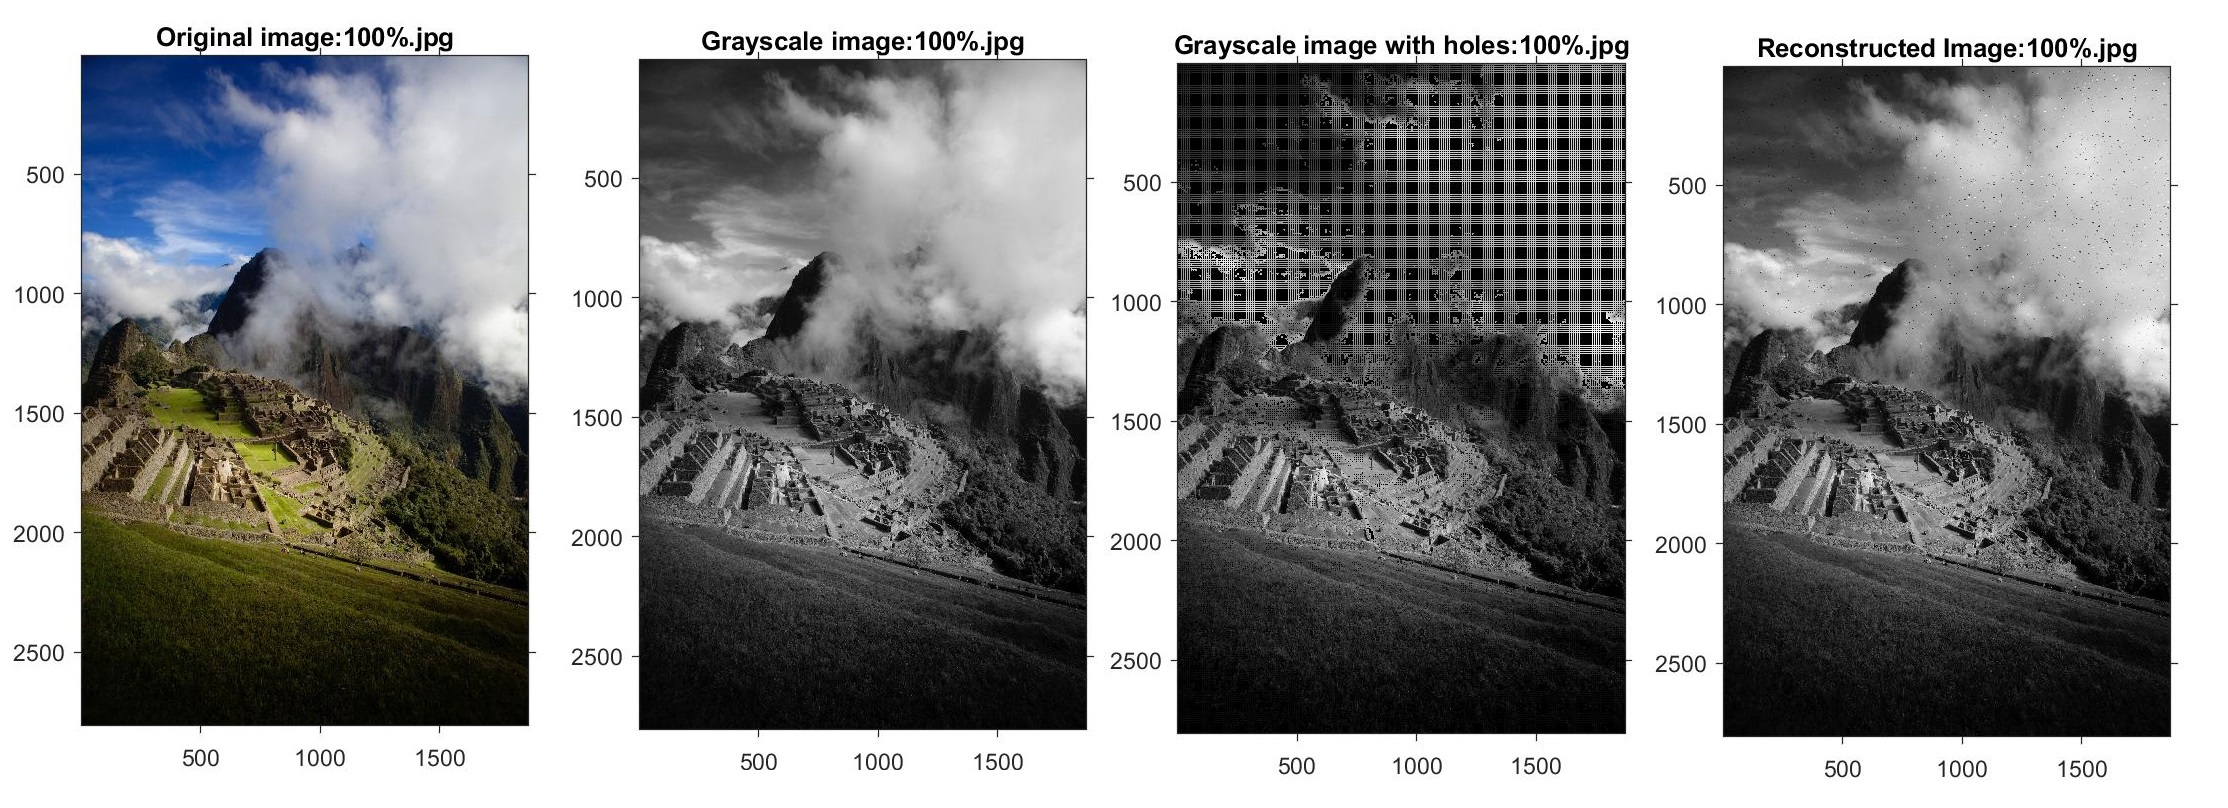
\includegraphics[scale=0.31]{AmandaKerr100.jpg}
\caption{Amanda Kerr landscape image at 100\% of the original size with 10\% error introduction}
\label{fig:AmandaKerr100}
\end{figure}

%% Pietro De Grandi

\begin{figure}[!ht]
\center 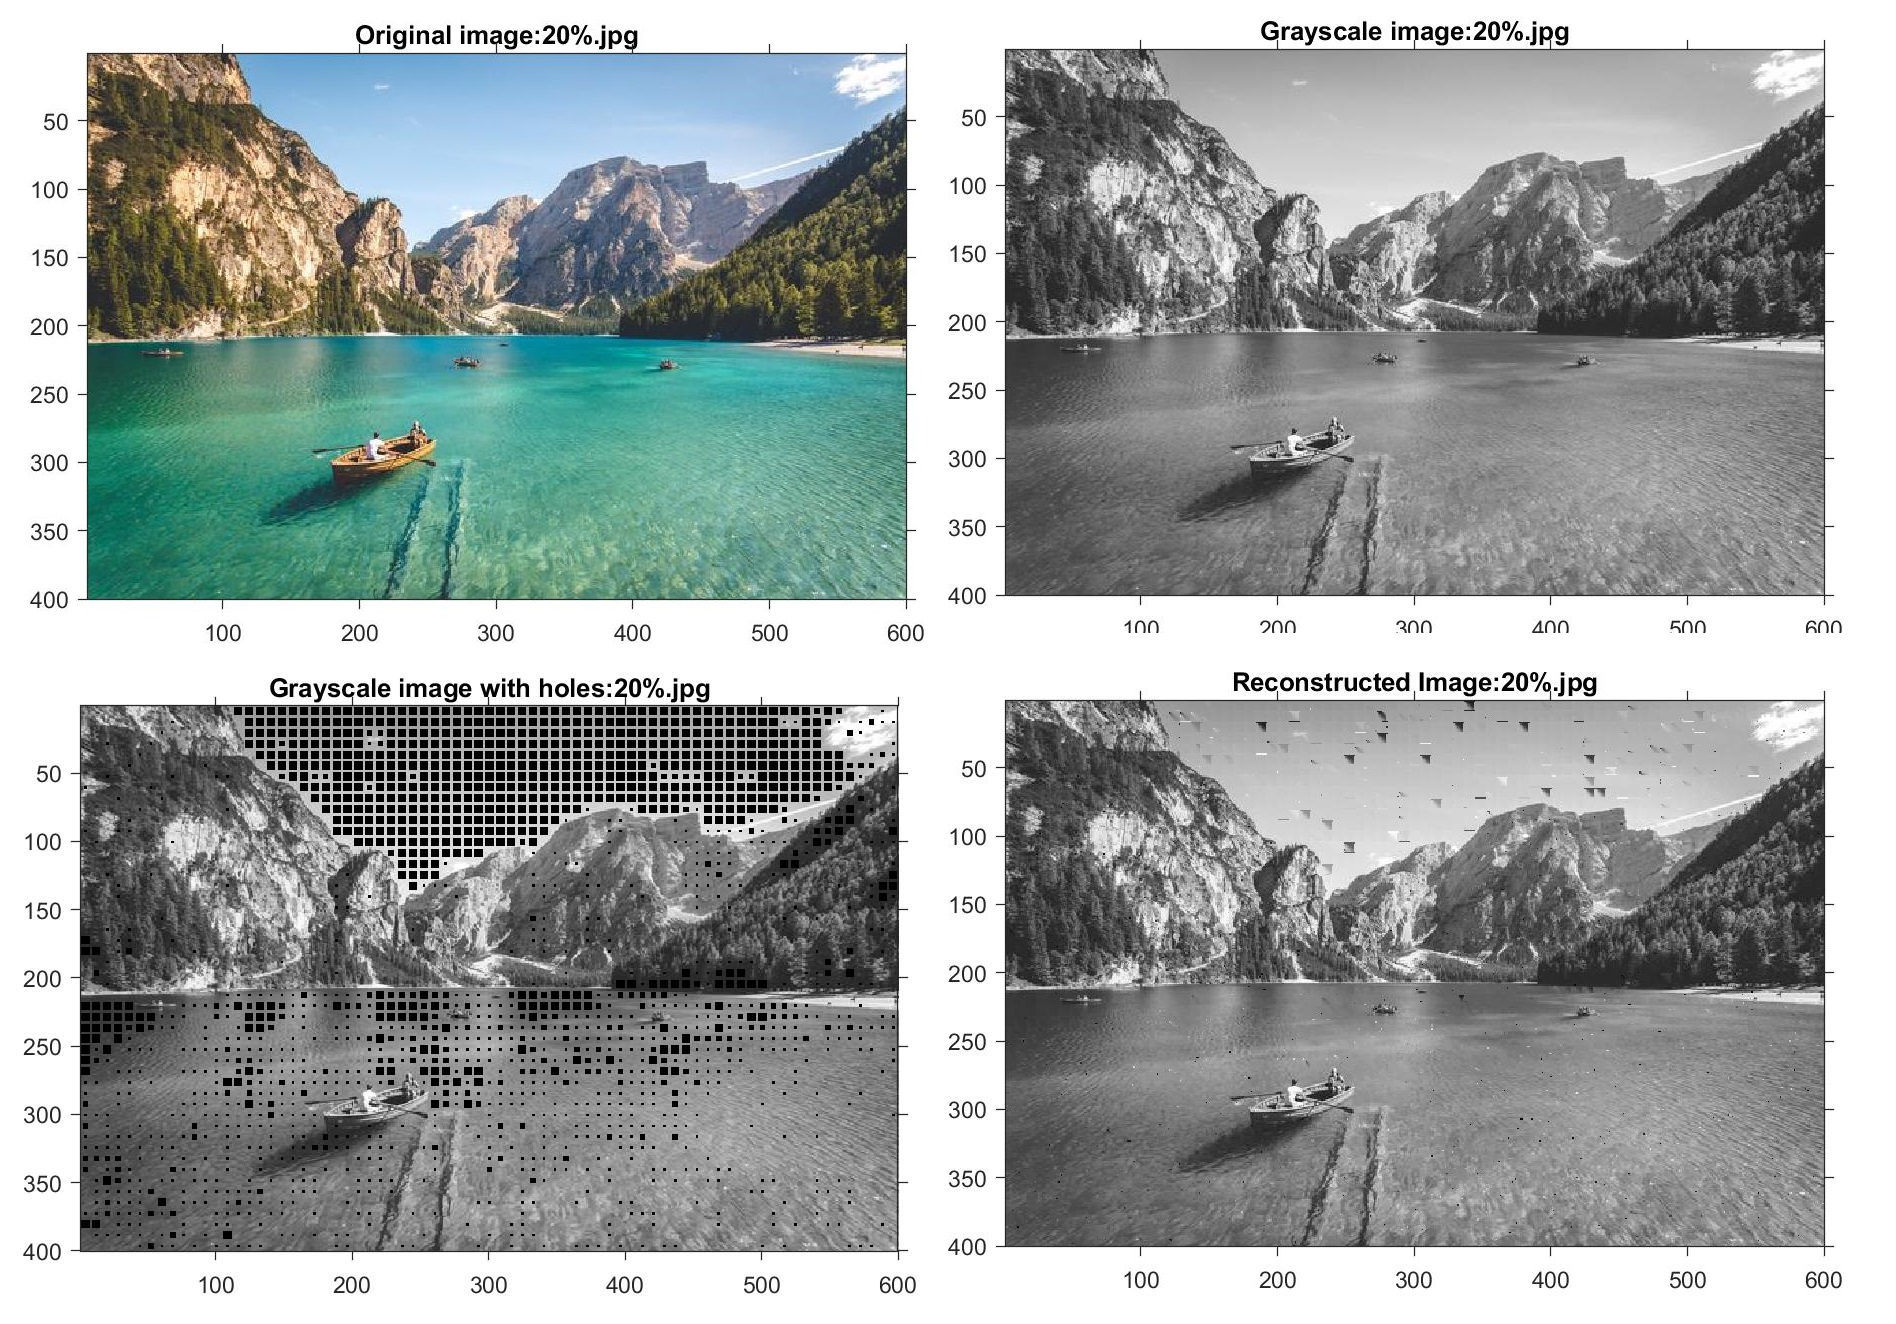
\includegraphics[scale=0.31]{PietroDeGrandi20.jpg}
\caption{Pietro De Grandi landscape image at 20\% of the original size with 10\% error introduction}
\label{fig:PietroDeGrandi20}
\end{figure}

\begin{figure}[!ht]
\center 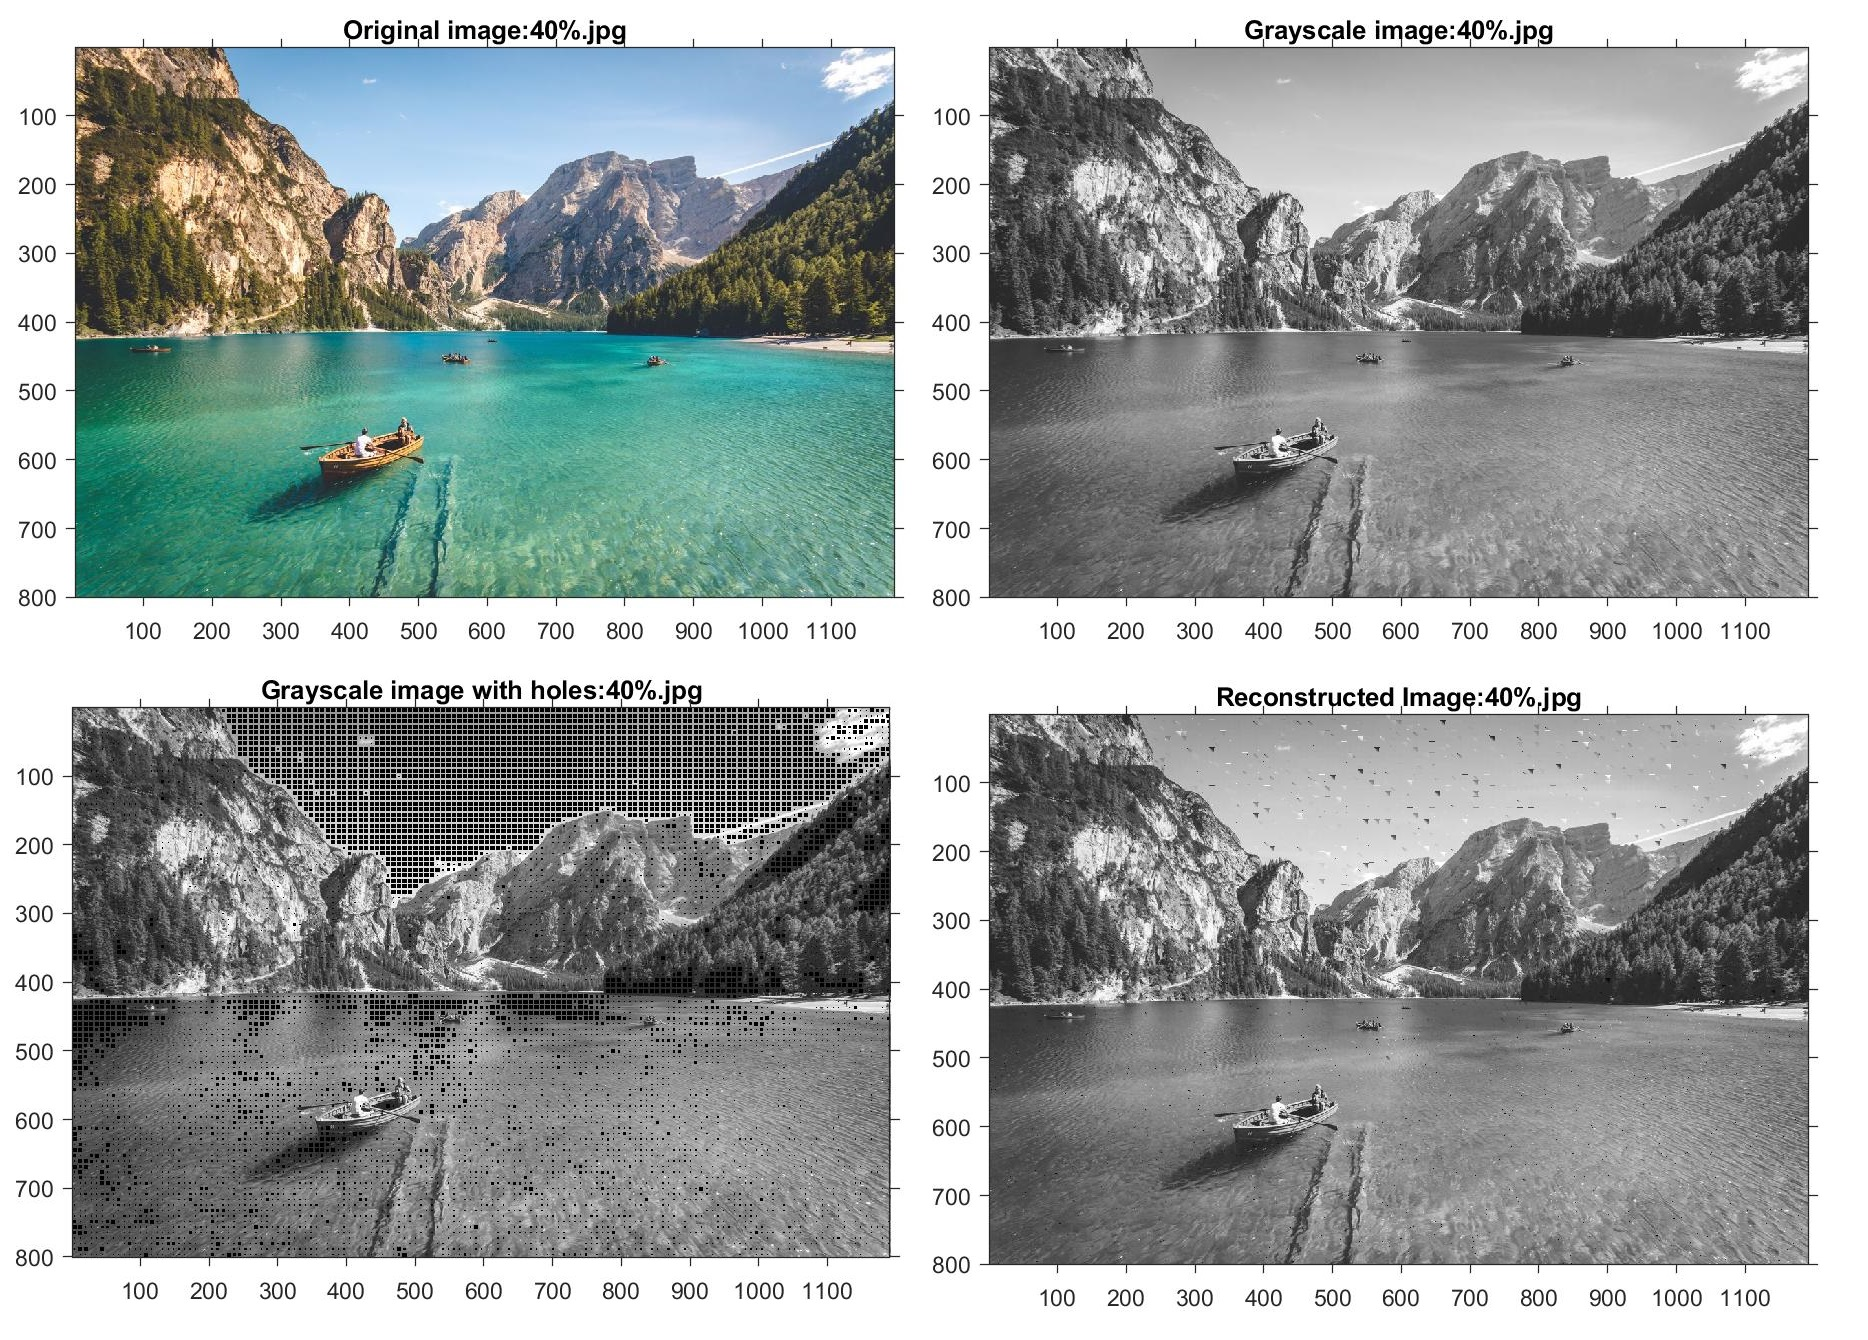
\includegraphics[scale=0.31]{PietroDeGrandi40.jpg}
\caption{Pietro De Grandi landscape image at 40\% of the original size with 40\% error introduction}
\label{fig:PietroDeGrandi20}
\end{figure}

\begin{figure}[!ht]
\center 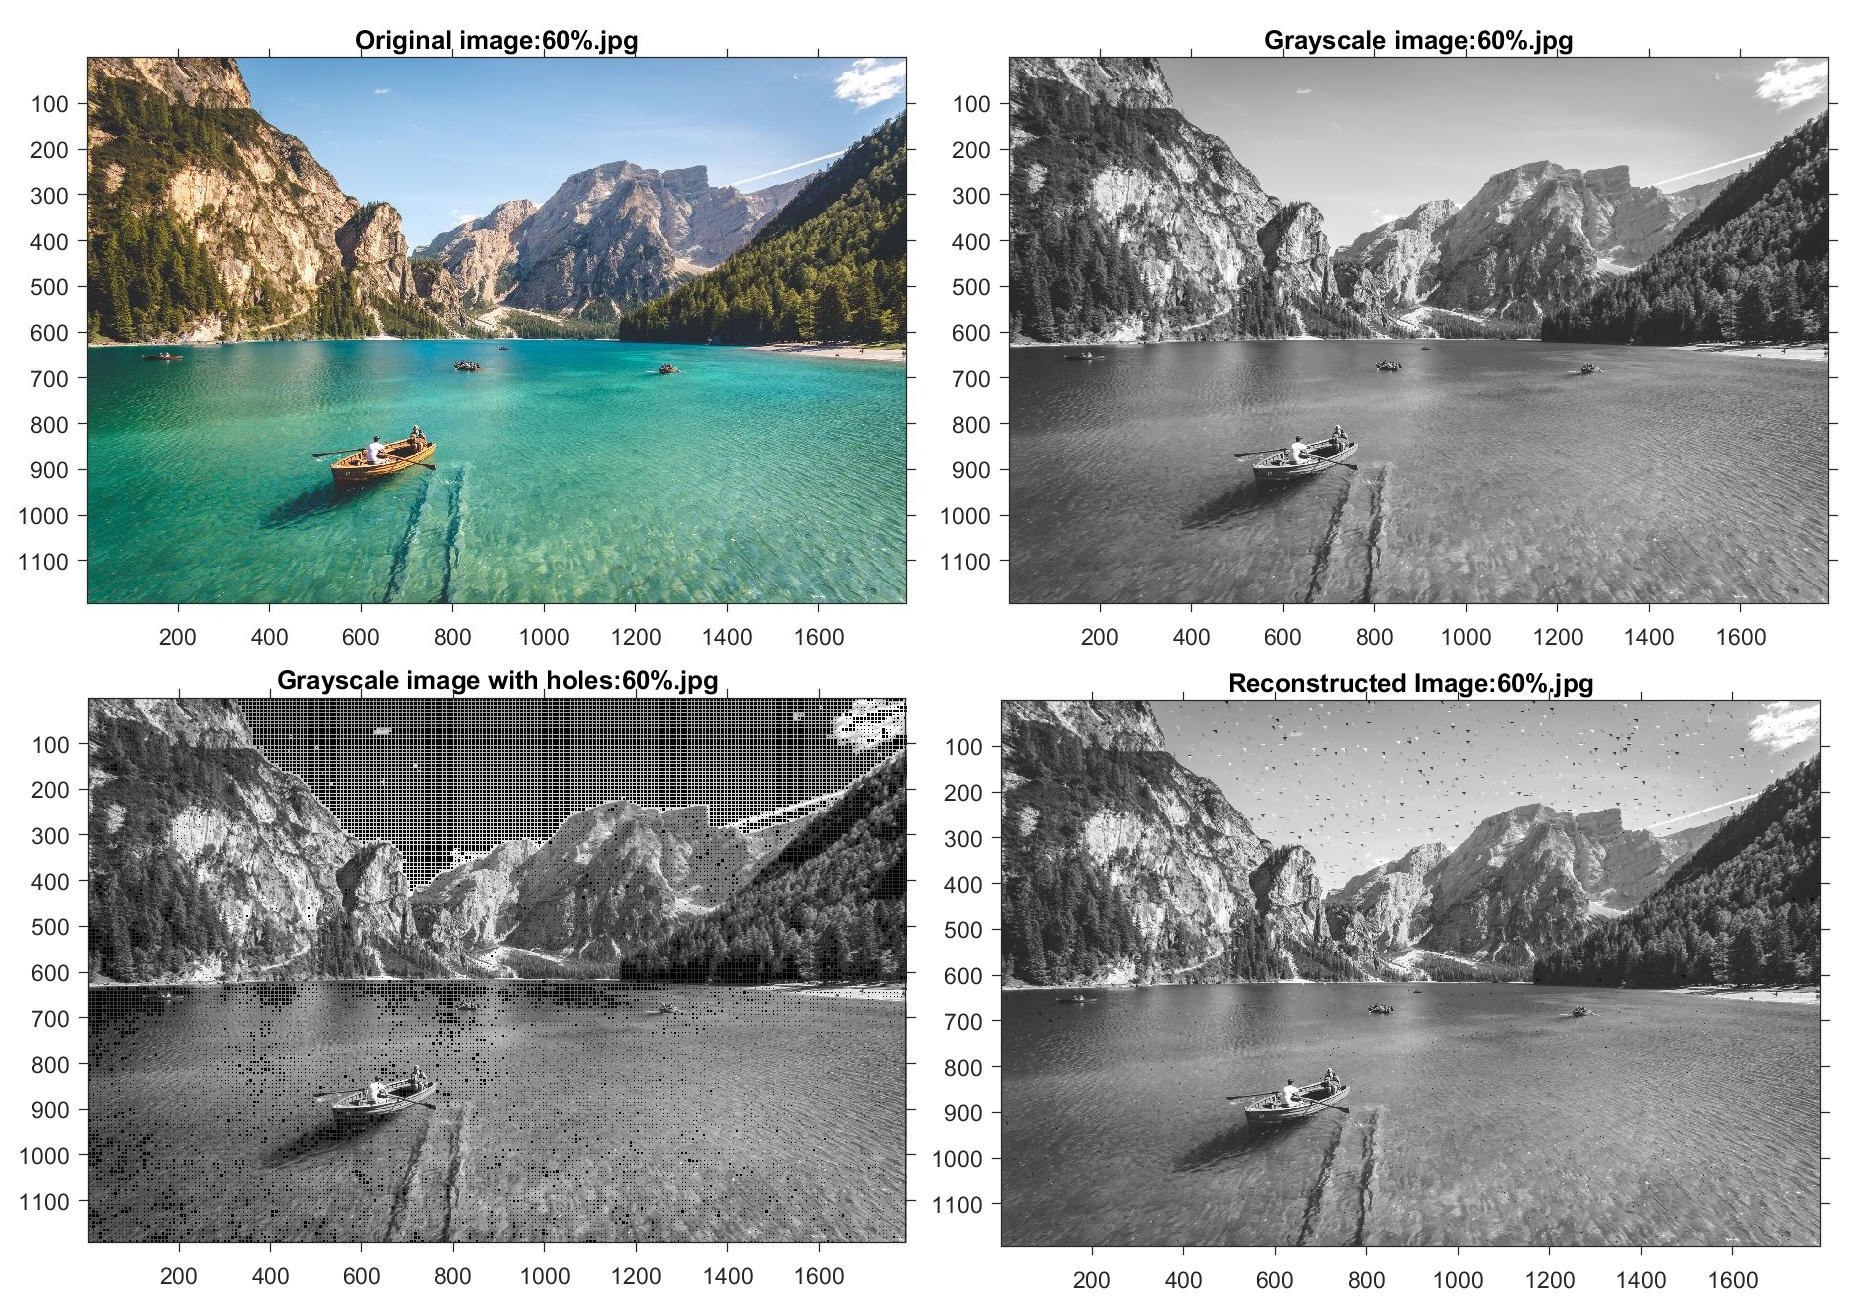
\includegraphics[scale=0.31]{PietroDeGrandi60.jpg}
\caption{Pietro De Grandi landscape image at 60\% of the original size with 60\% error introduction}
\label{fig:PietroDeGrandi20}
\end{figure}

\begin{figure}[!ht]
\center 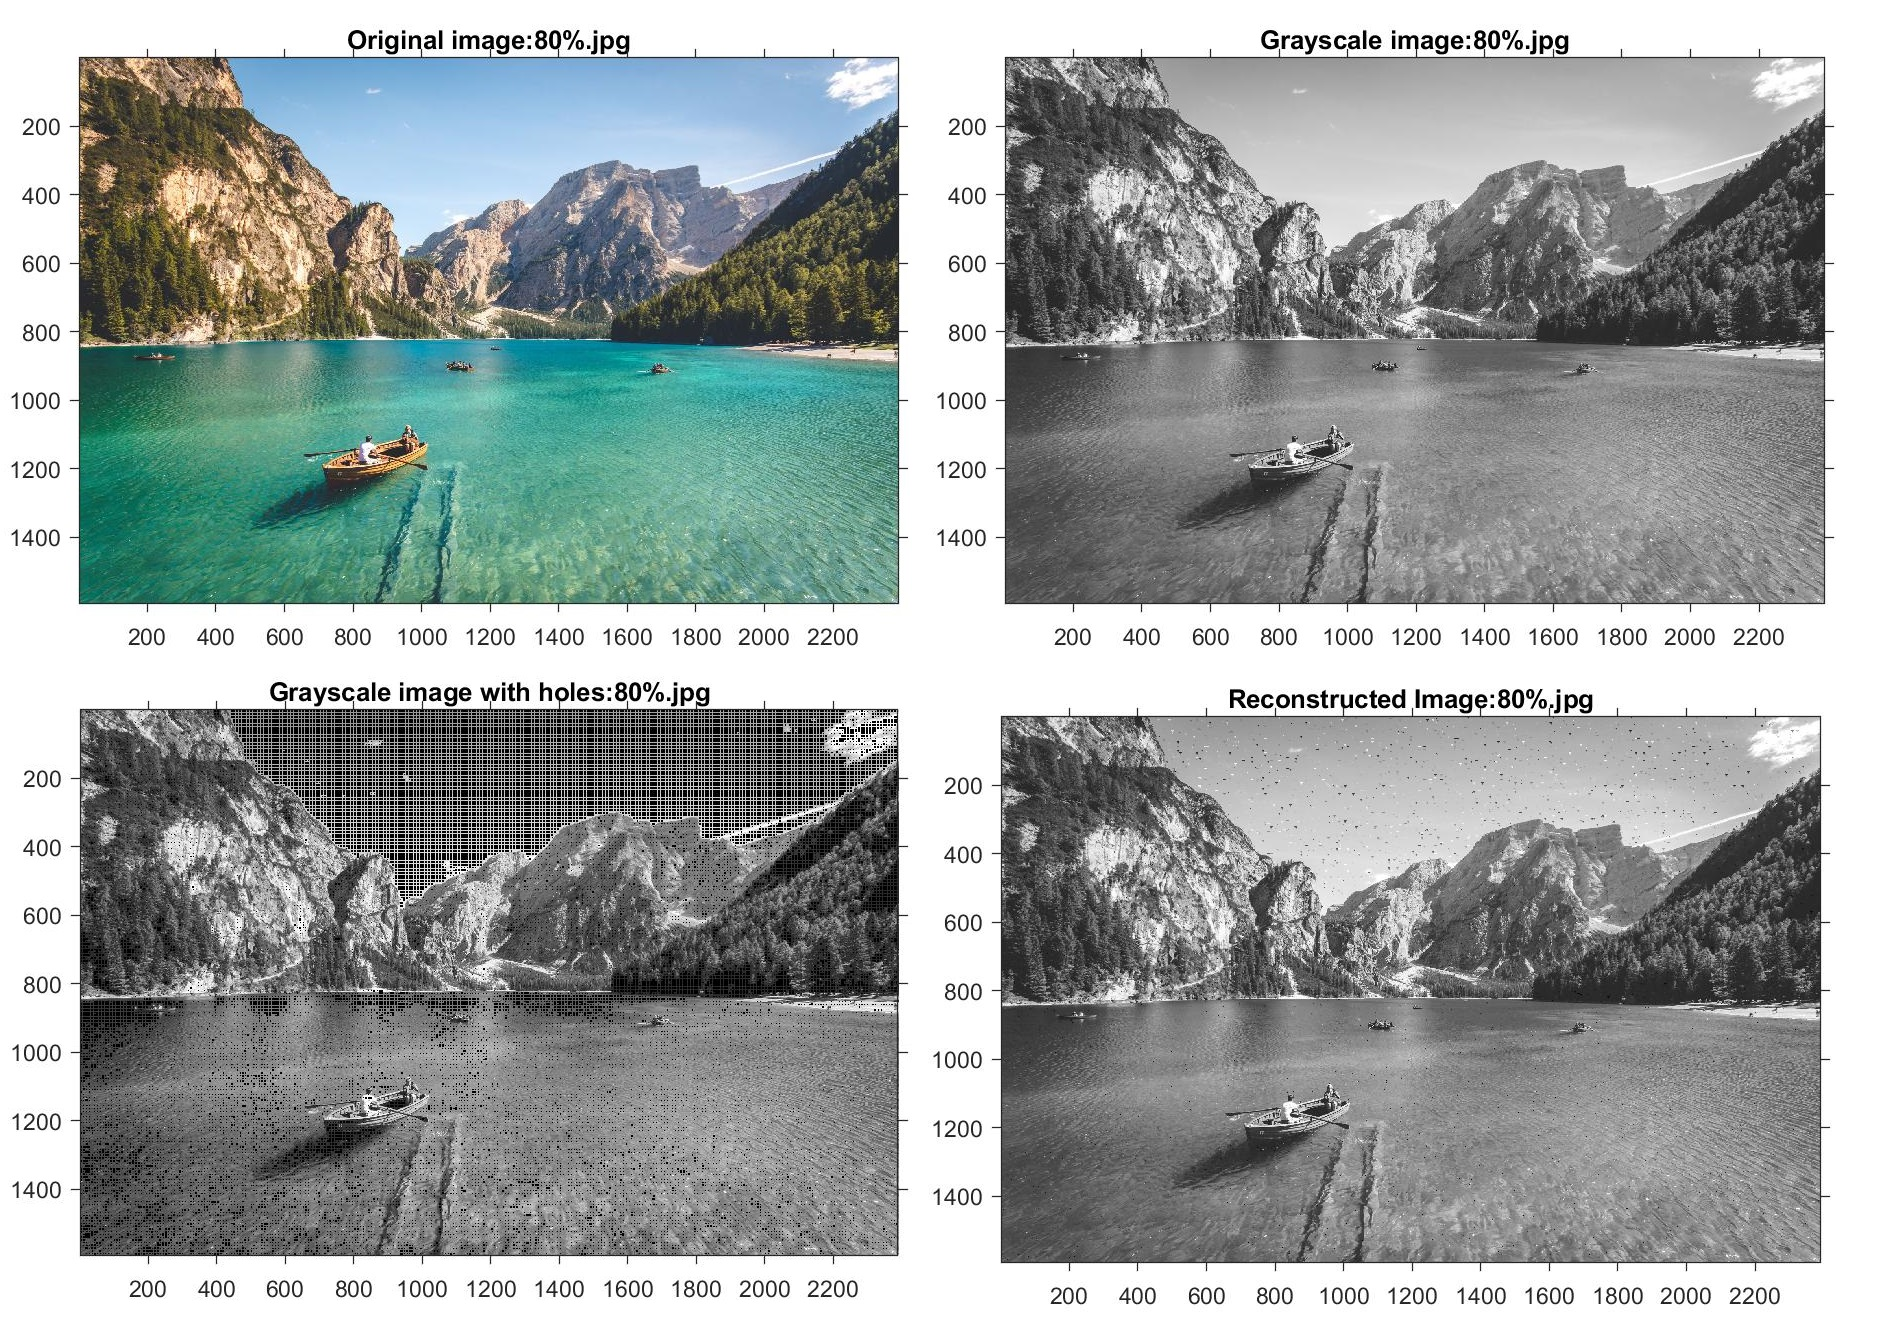
\includegraphics[scale=0.31]{PietroDeGrandi80.jpg}
\caption{Pietro De Grandi landscape image at 80\% of the original size with 10\% error introduction}
\label{fig:PietroDeGrandi80}
\end{figure}

\begin{figure}[!ht]
\center 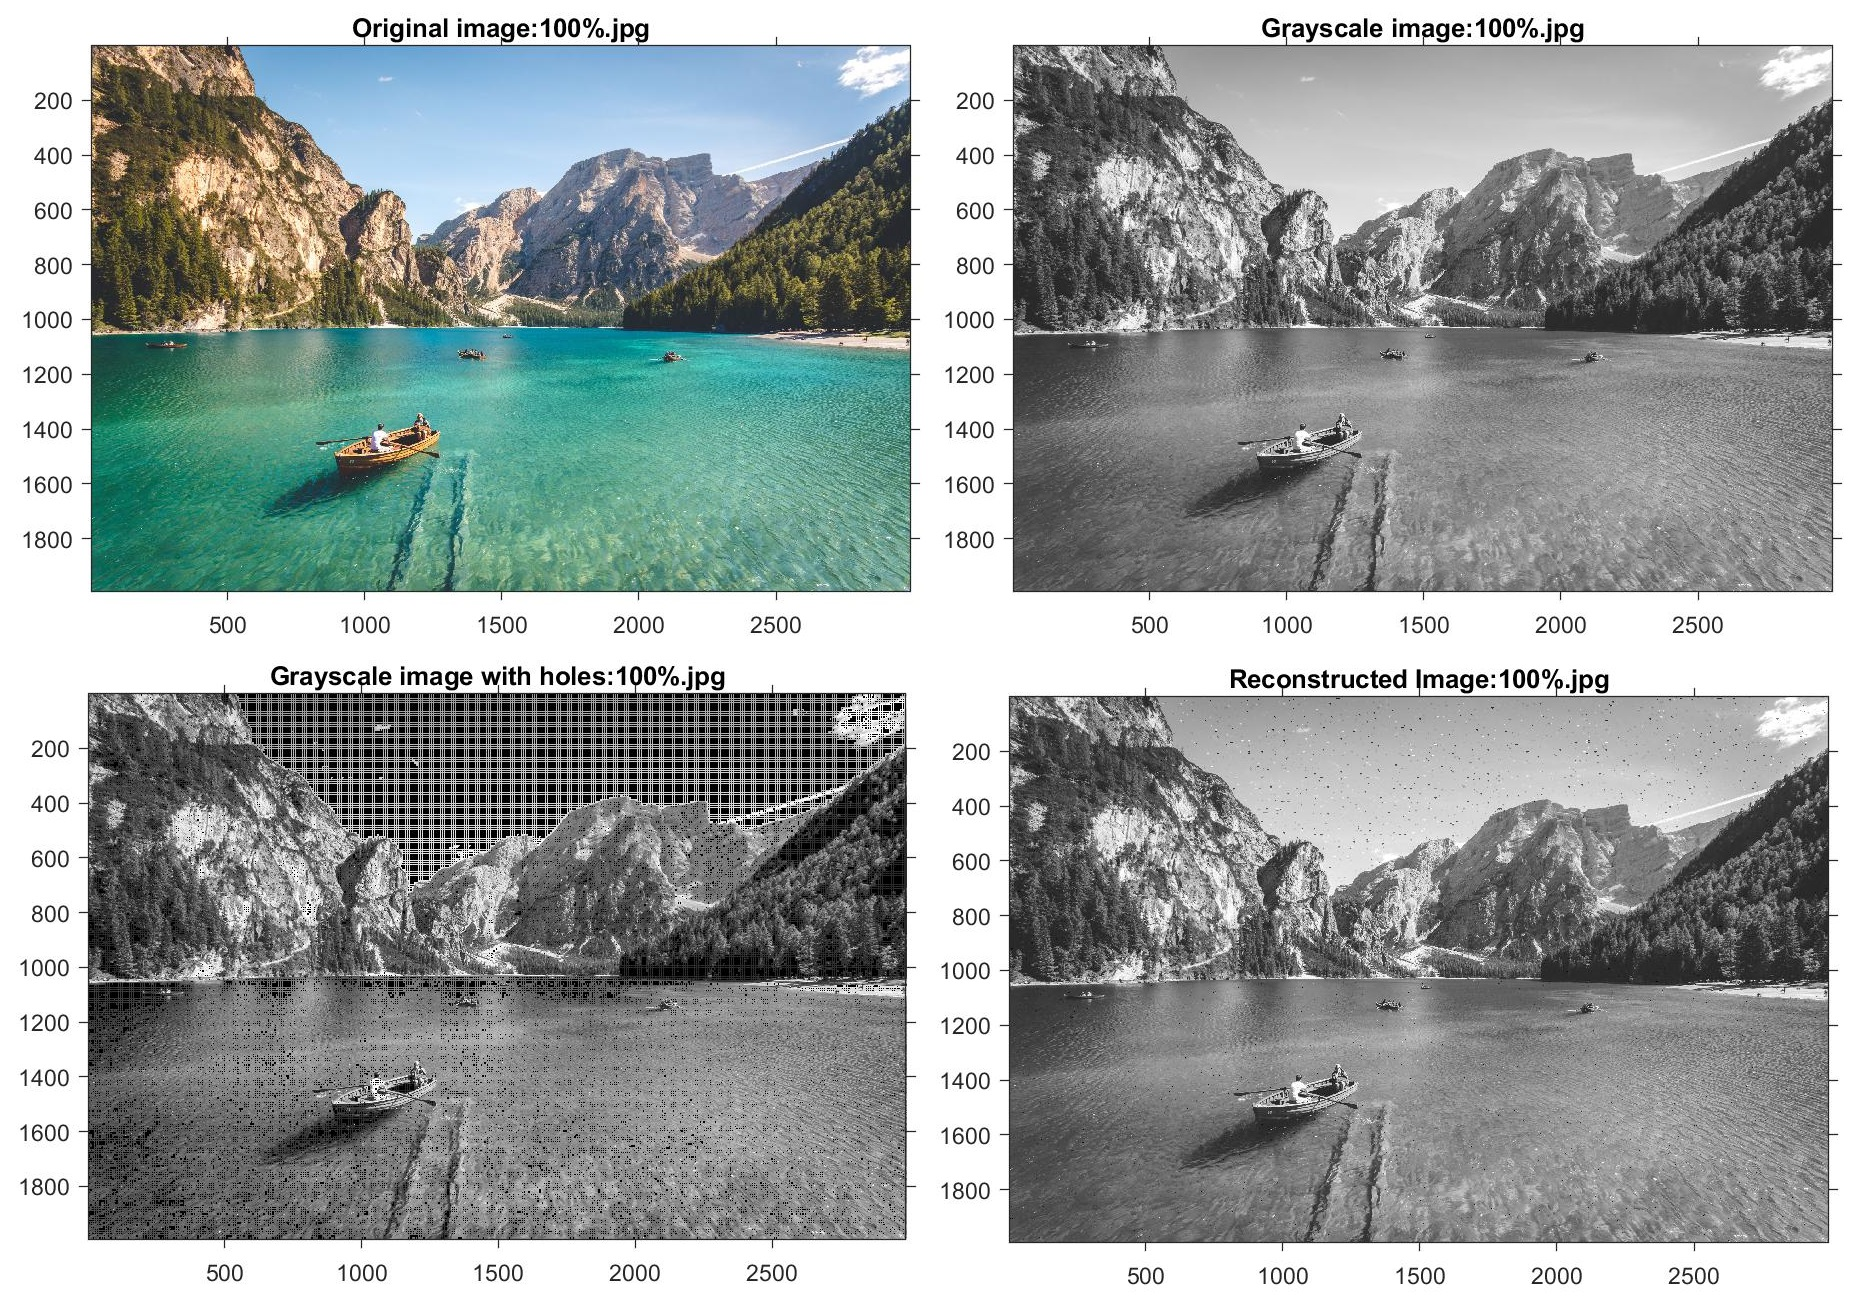
\includegraphics[scale=0.31]{PietroDeGrandi100.jpg}
\caption{Pietro De Grandi landscape image at 100\% of the original size with 10\% error introduction}
\label{fig:PietroDeGrandi100}
\end{figure}

%% Simon Matzinger

\begin{figure}[!ht]
\center 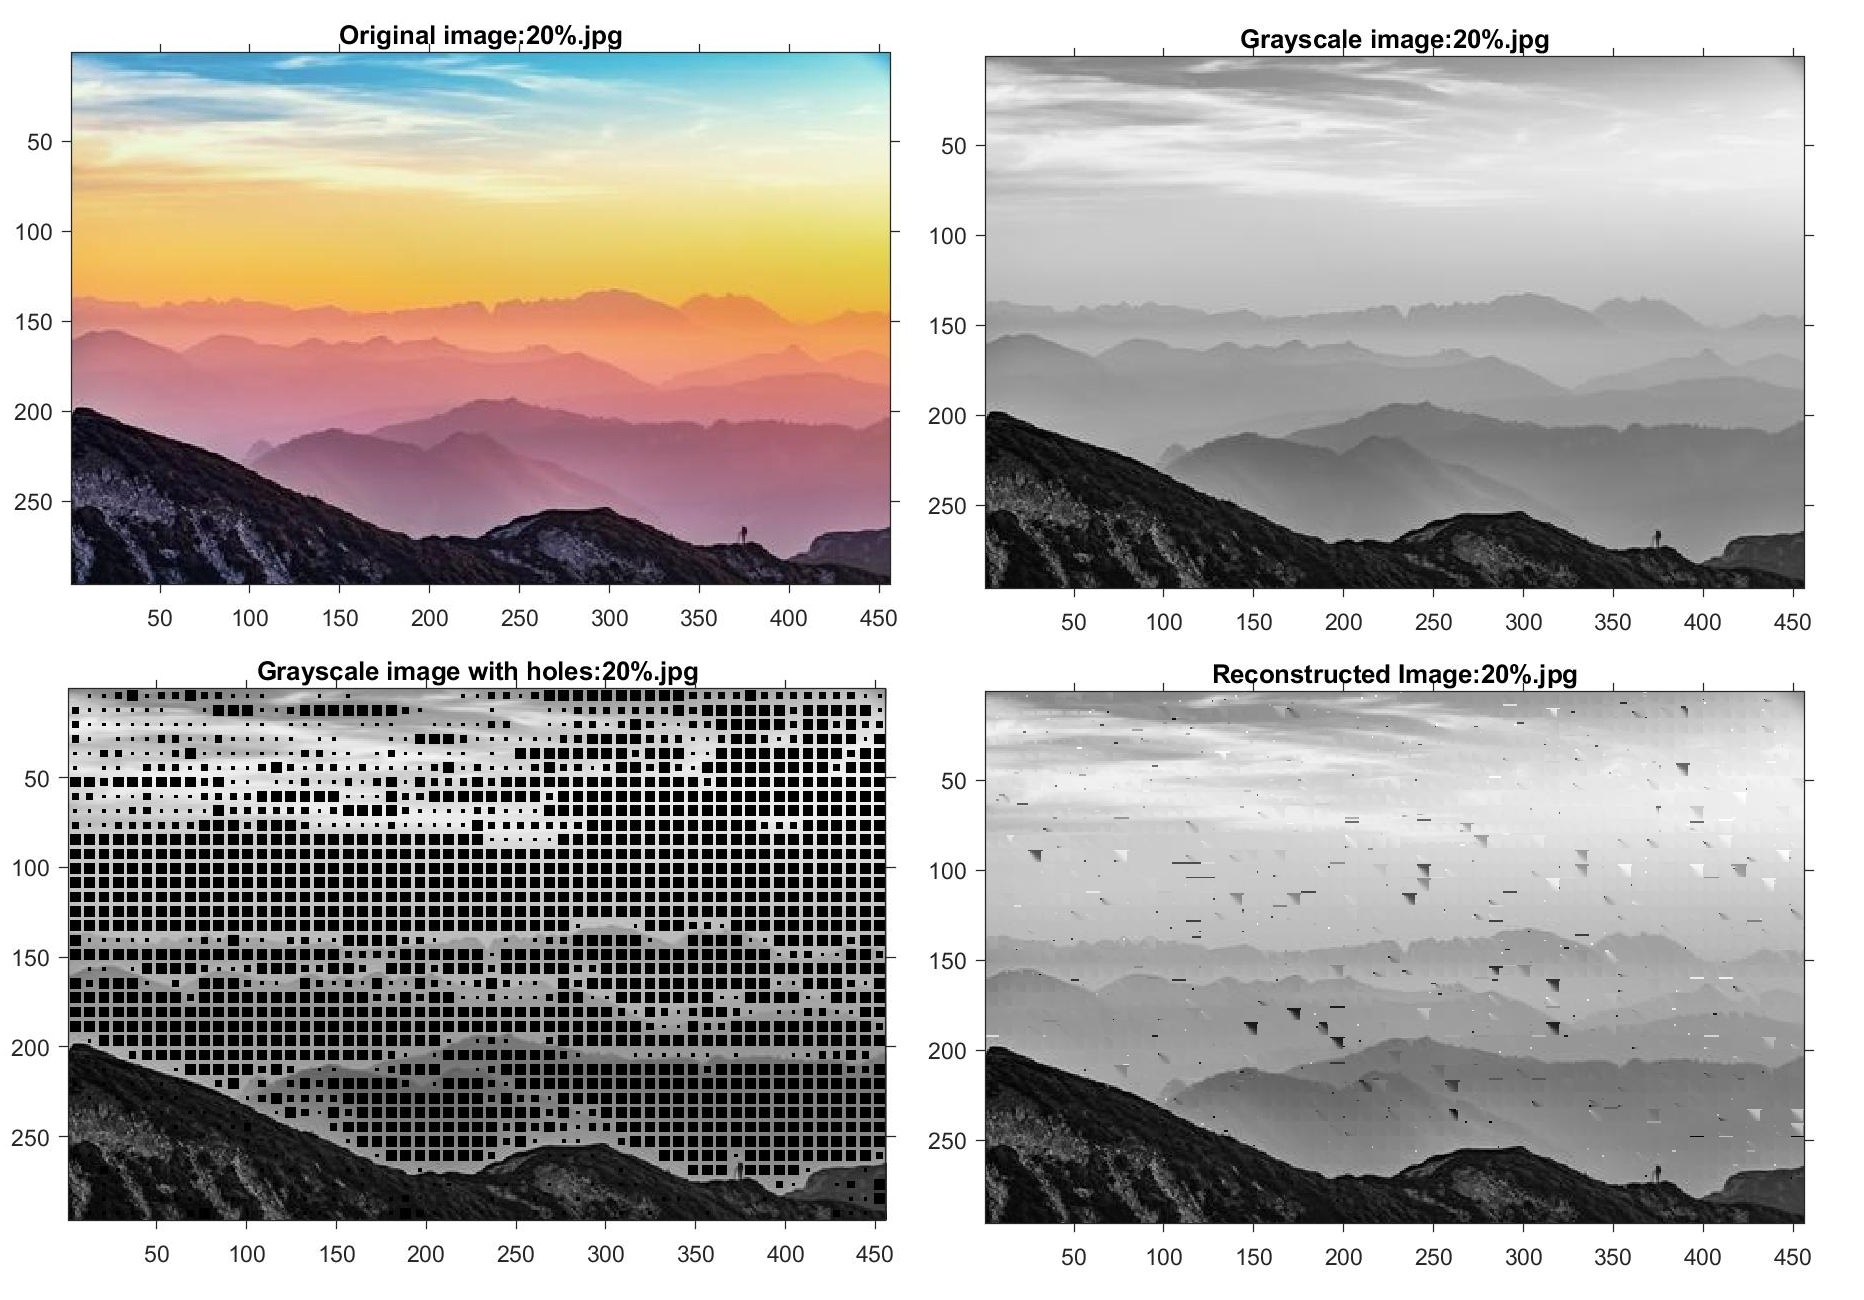
\includegraphics[scale=0.31]{SimonMatzinger20.jpg}
\caption{Simon Matzinger landscape image at 20\% of the original size with 10\% error introduction}
\label{fig:SimonMatzinger20}
\end{figure}

\begin{figure}[!ht]
\center 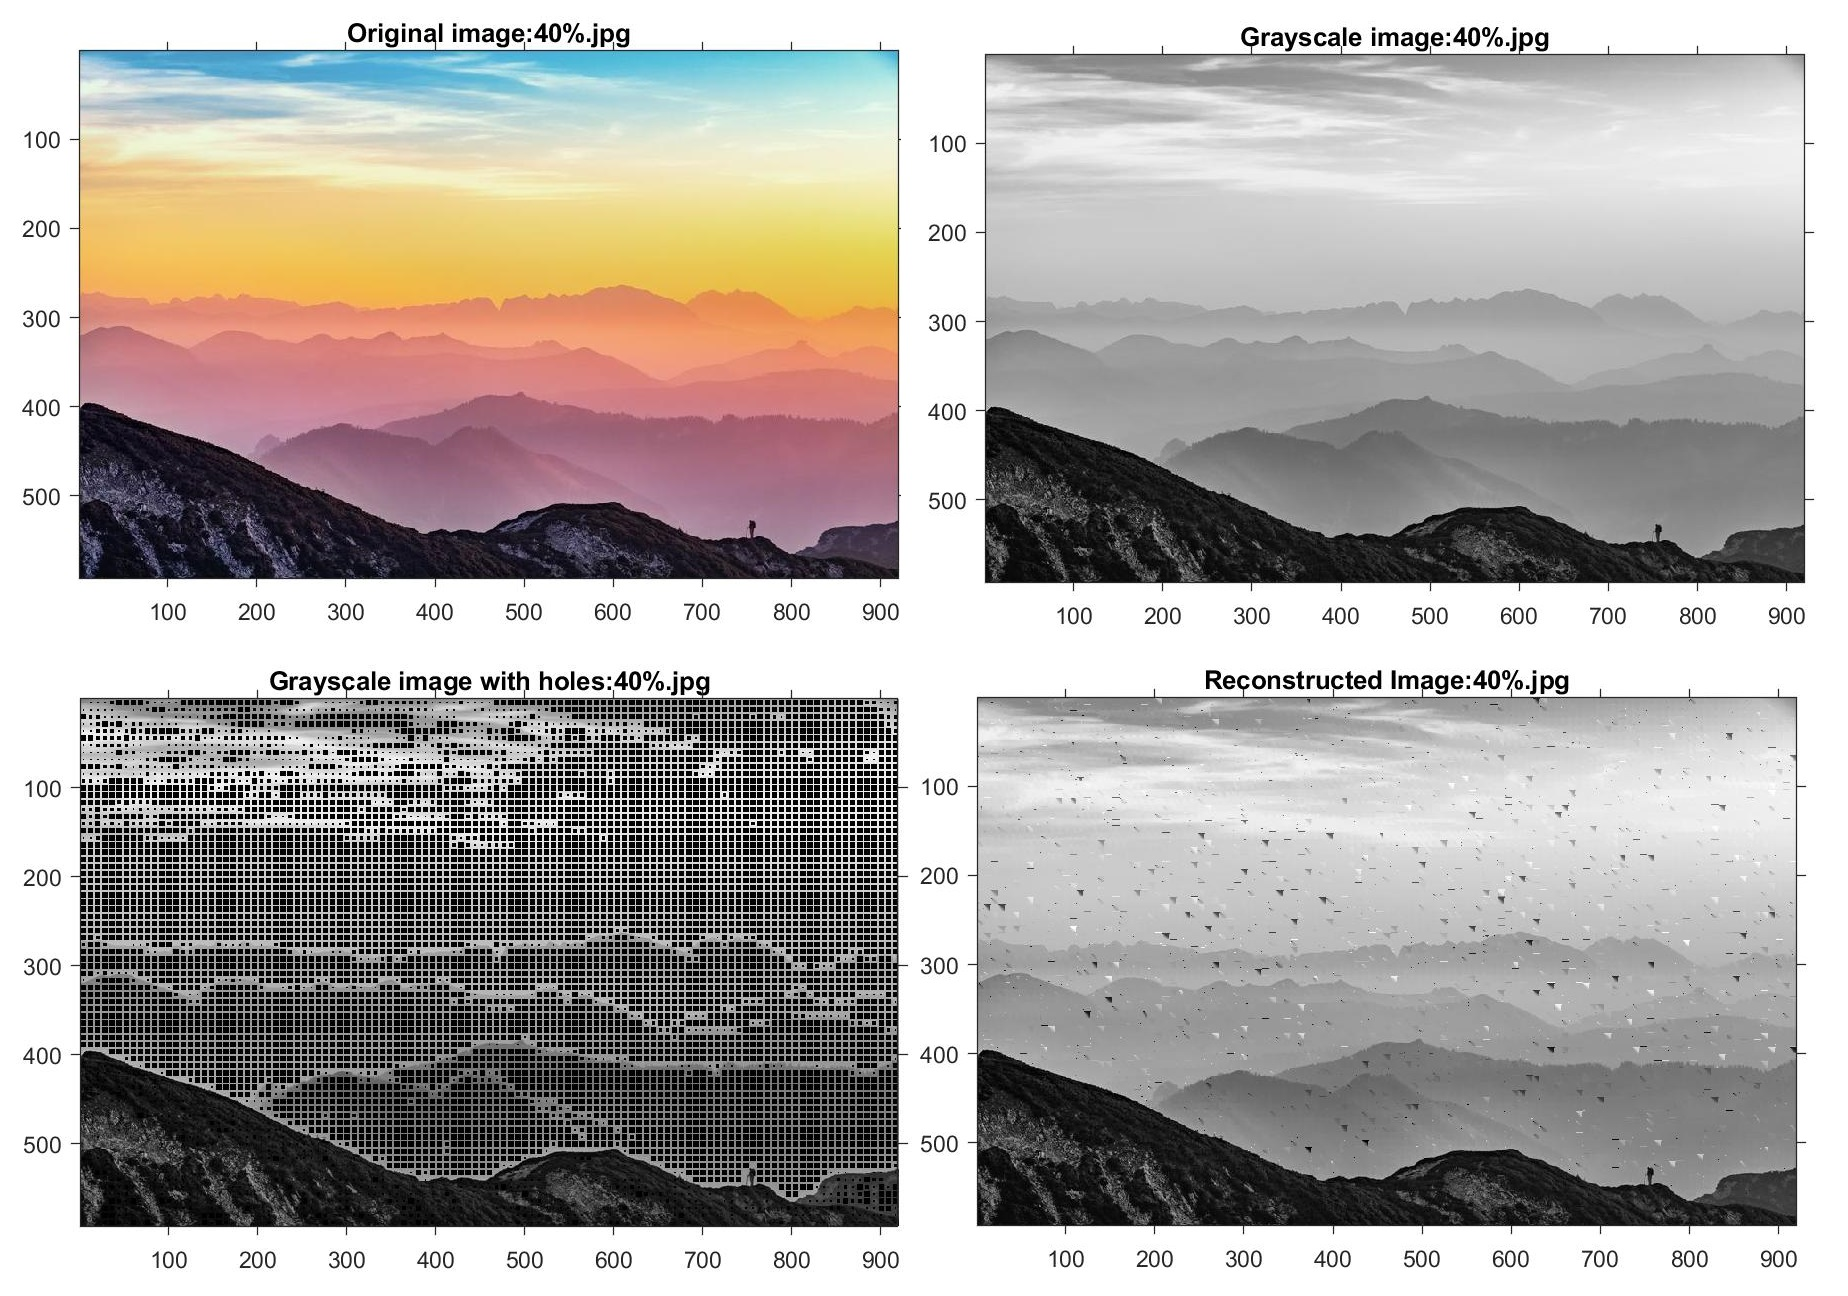
\includegraphics[scale=0.31]{SimonMatzinger40.jpg}
\caption{Simon Matzinger landscape image at 40\% of the original size with 10\% error introduction}
\label{fig:SimonMatzinger40}
\end{figure}

\begin{figure}[!ht]
\center 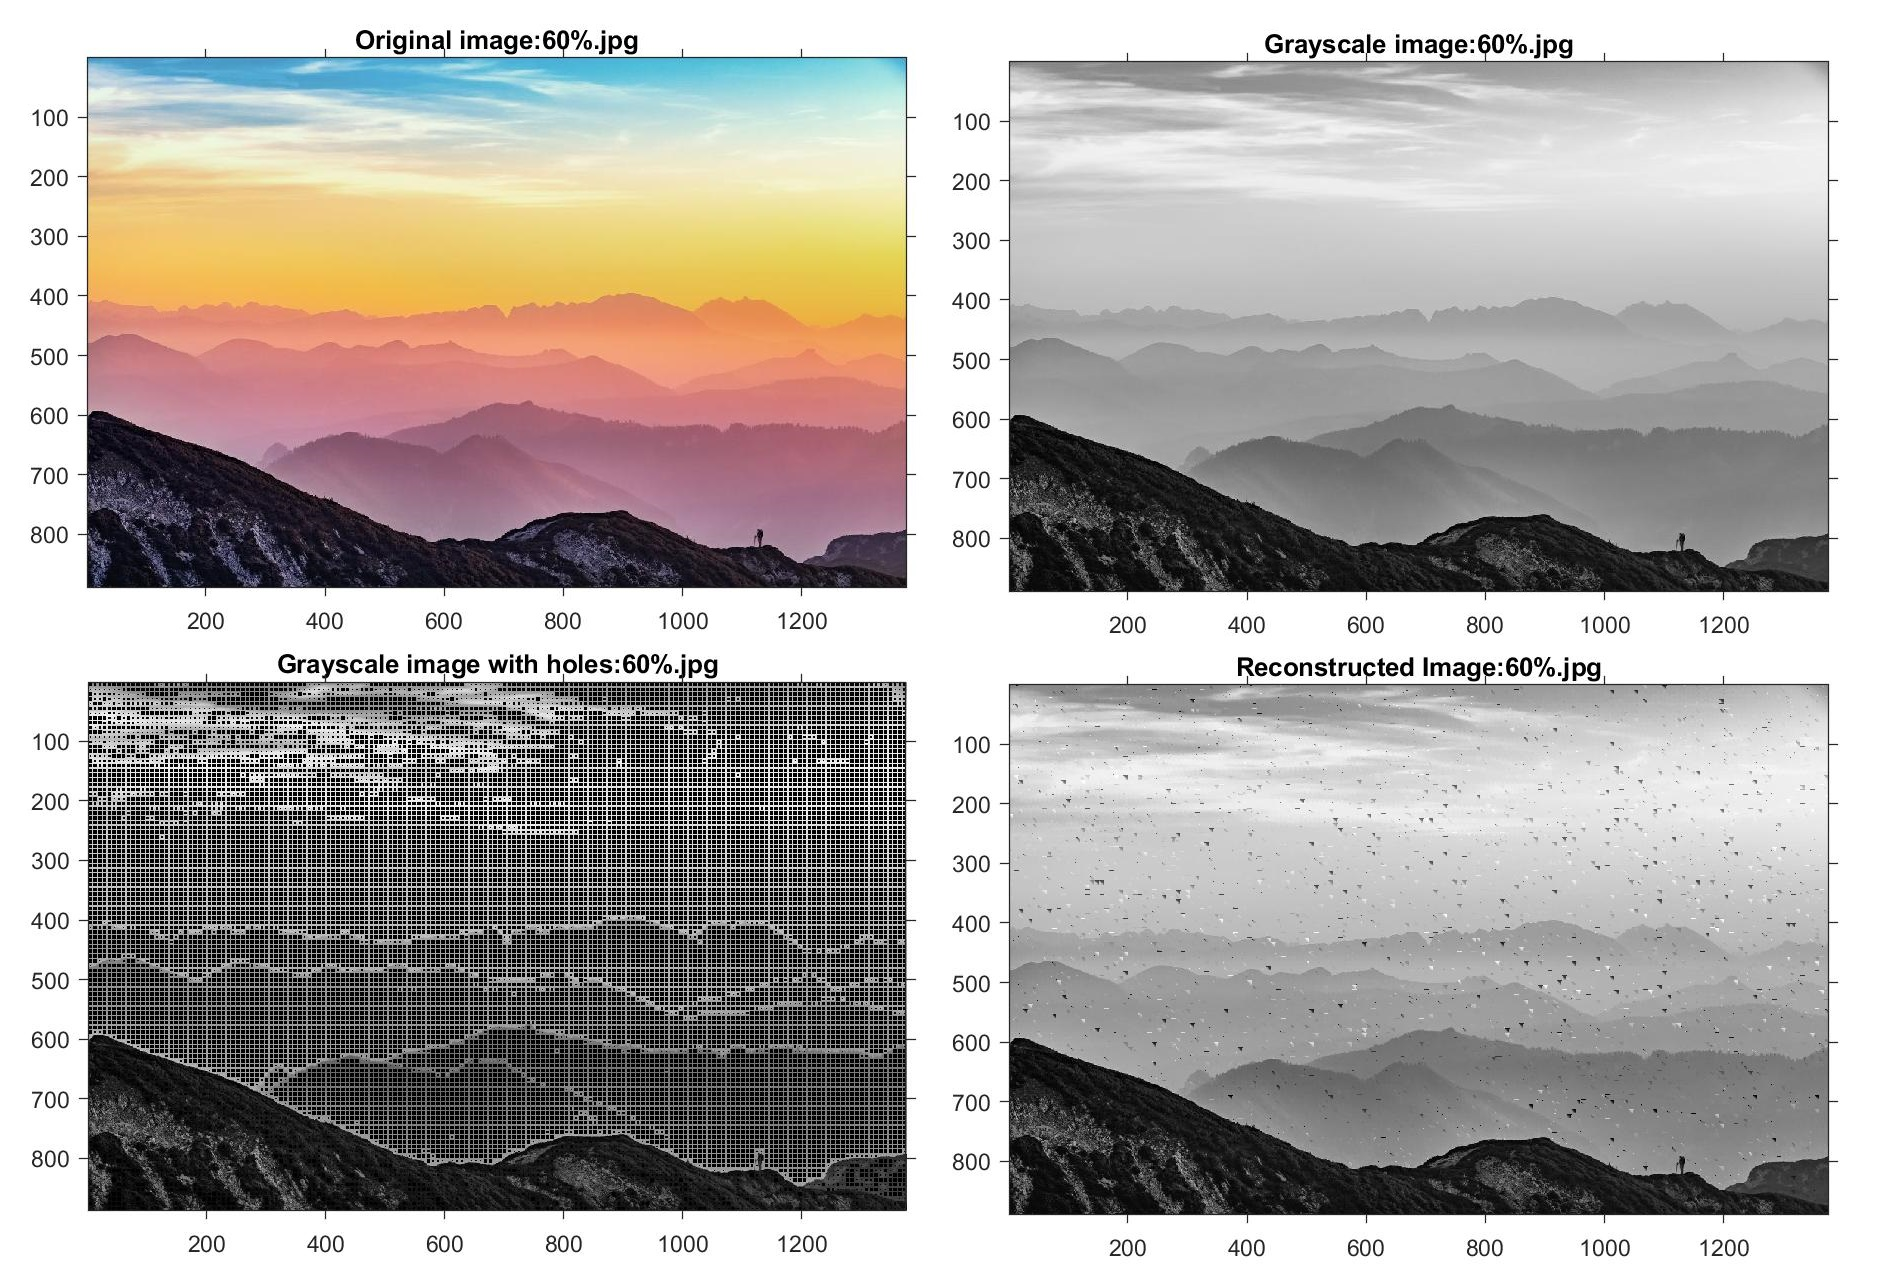
\includegraphics[scale=0.31]{SimonMatzinger60.jpg}
\caption{Simon Matzinger landscape image at 60\% of the original size with 10\% error introduction}
\label{fig:SimonMatzinger60}
\end{figure}

\begin{figure}[!ht]
\center 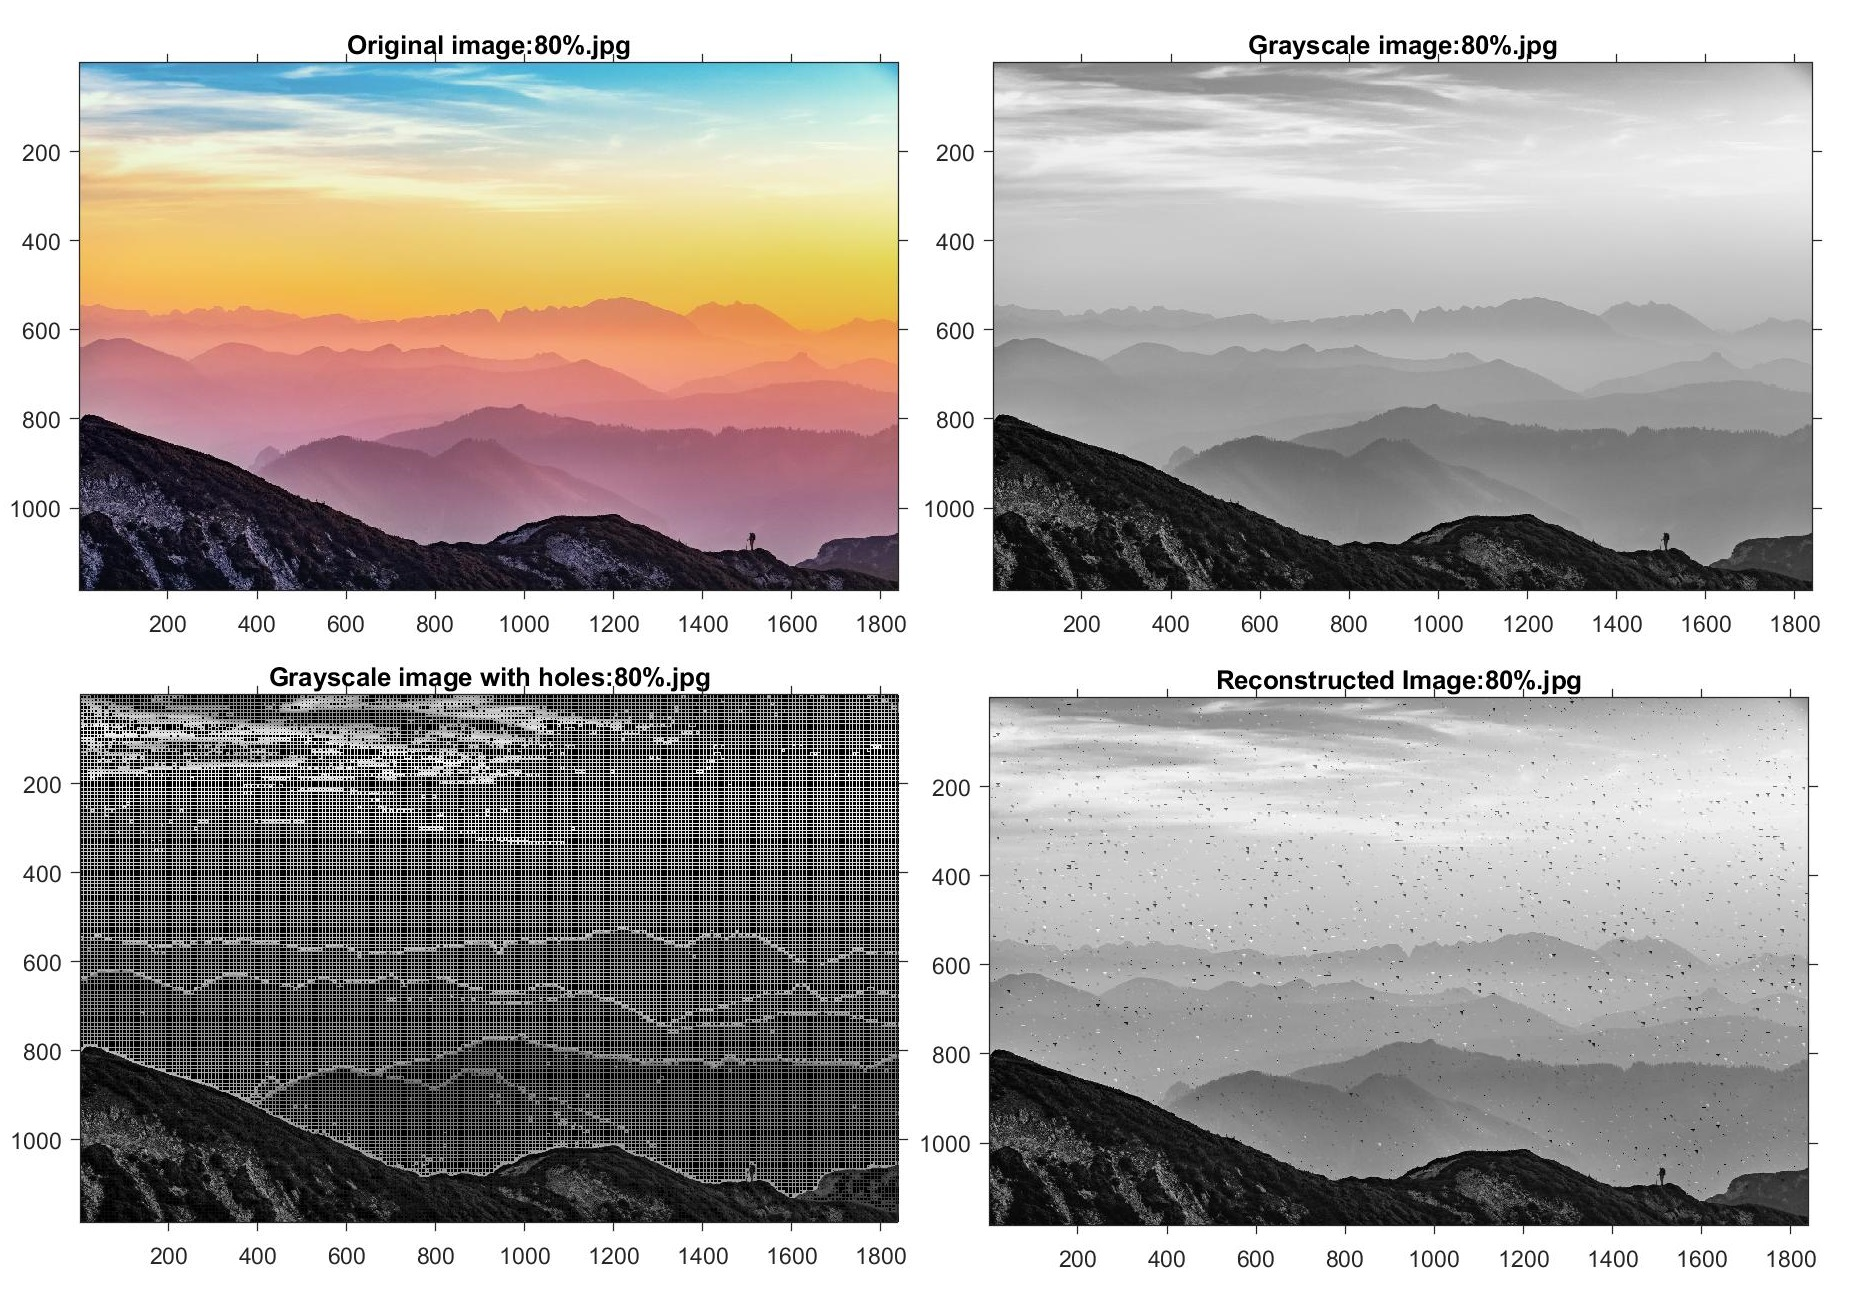
\includegraphics[scale=0.31]{SimonMatzinger80.jpg}
\caption{Simon Matzinger landscape image at 80\% of the original size with 10\% error introduction}
\label{fig:SimonMatzinger80}
\end{figure}

\begin{figure}[!ht]
\center 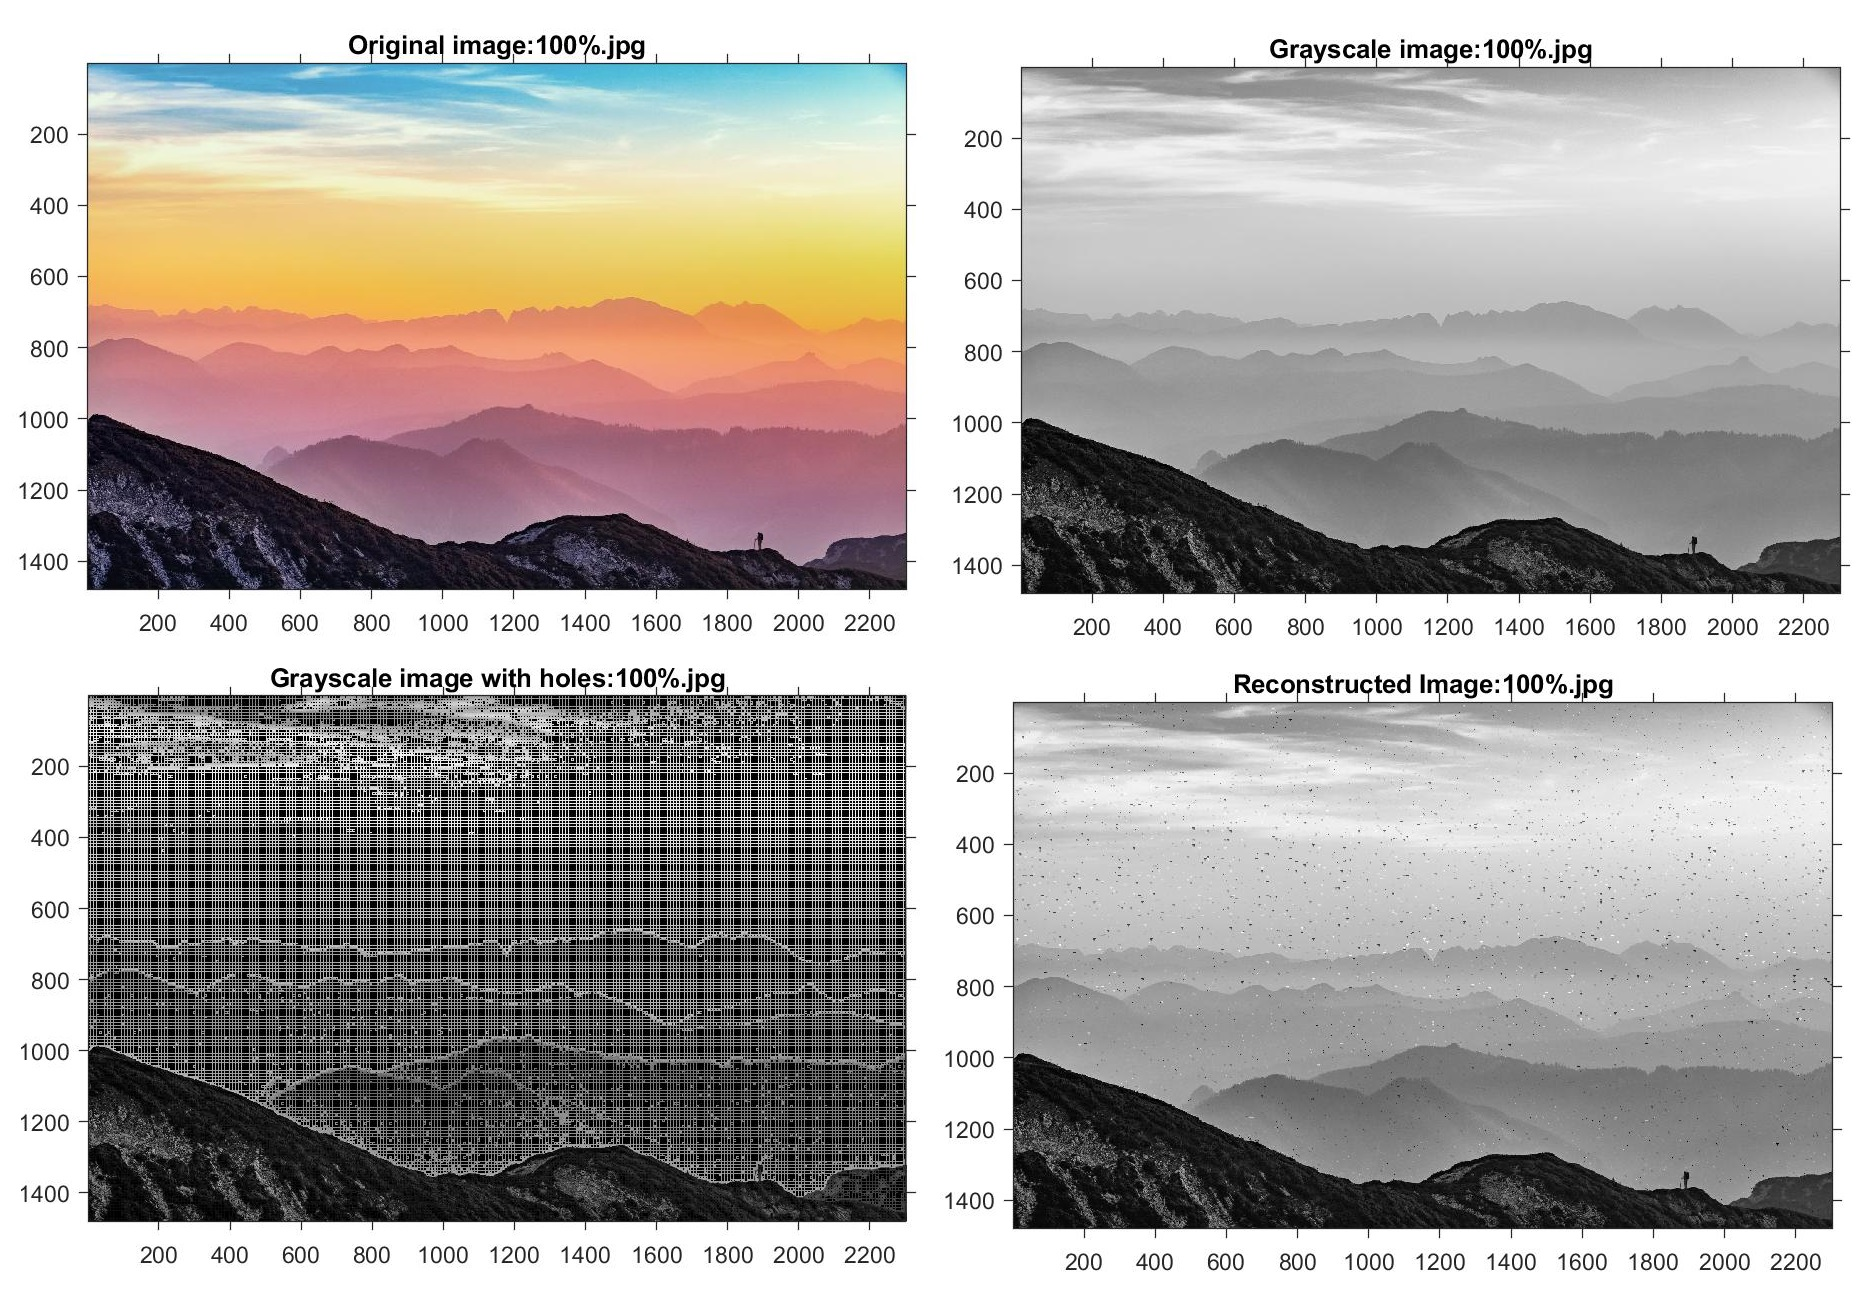
\includegraphics[scale=0.31]{SimonMatzinger100.jpg}
\caption{Simon Matzinger landscape image at 100\% of the original size with 10\% error introduction}
\label{fig:SimonMatzinger100}
\end{figure}

%%

%% PATTERN IMAGES

%% Andrej Lisakov

\begin{figure}[!ht]
\center 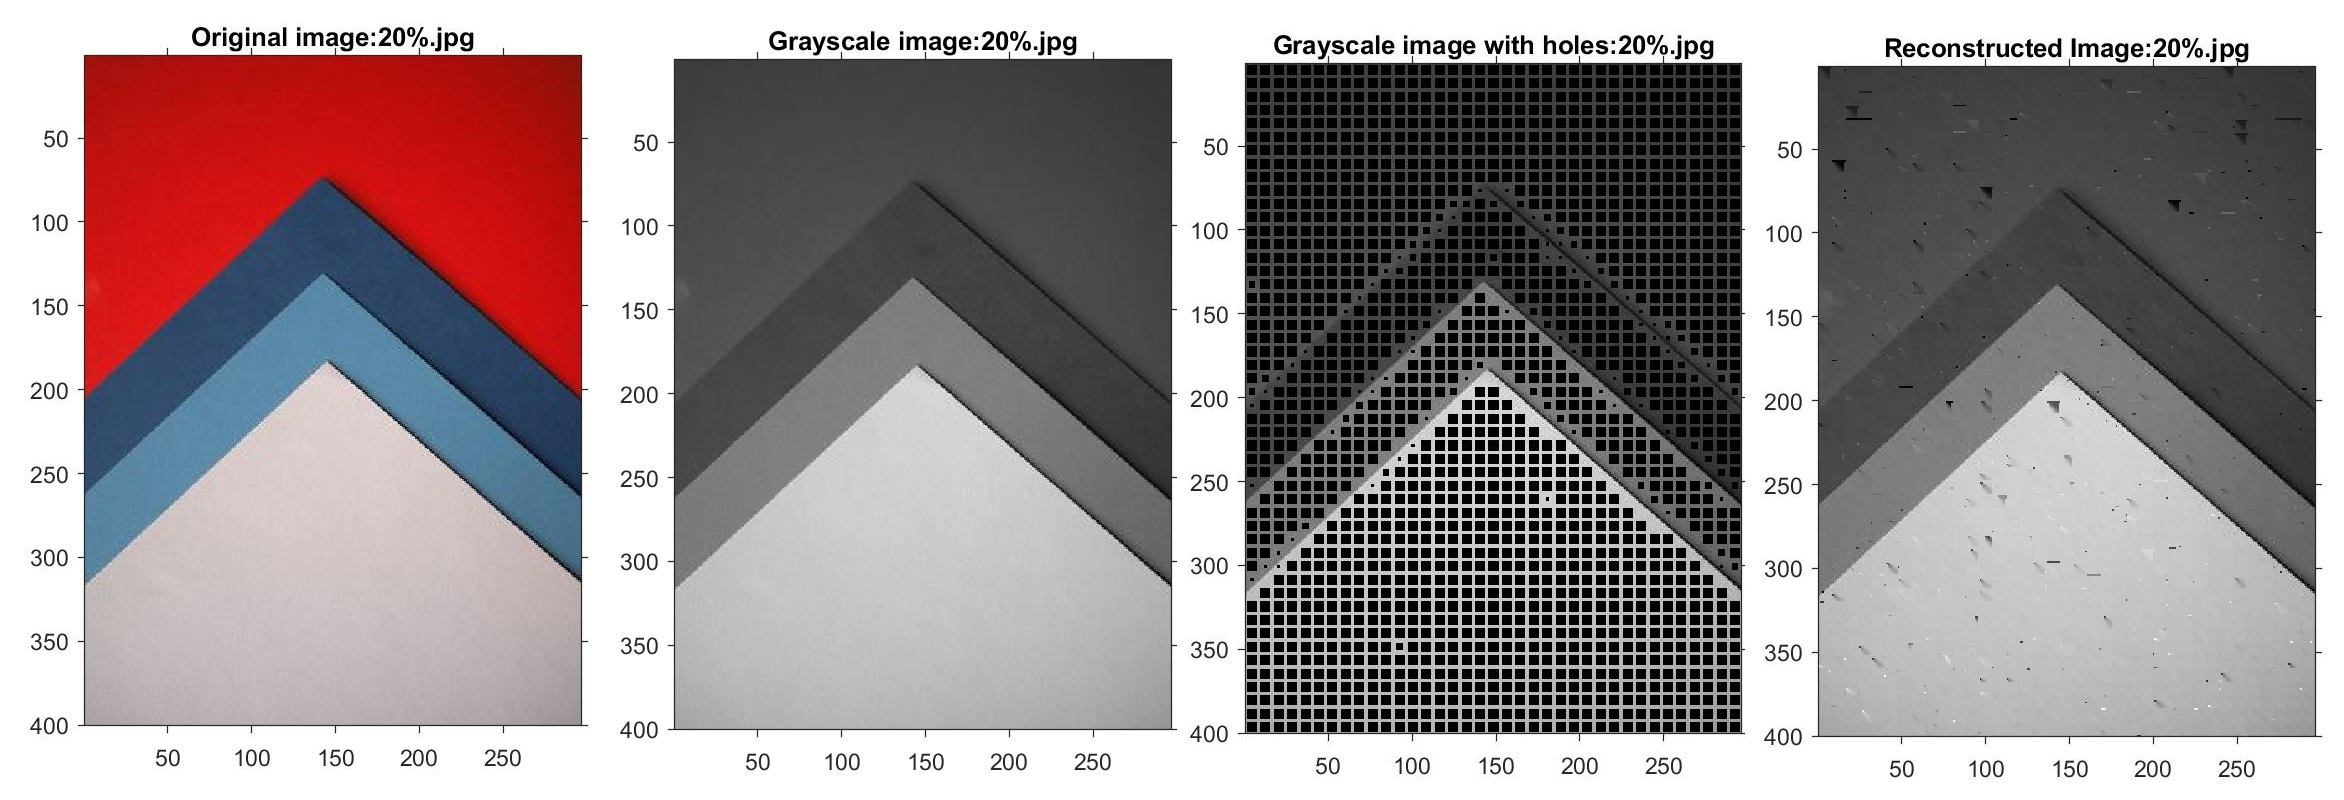
\includegraphics[scale=0.31]{AndrejLisakov20.jpg}
\caption{Andrej Lisakov texture image at 20\% of the original size with 10\% error introduction}
\label{fig:AndrejLisakov20}
\end{figure}

\begin{figure}[!ht]
\center 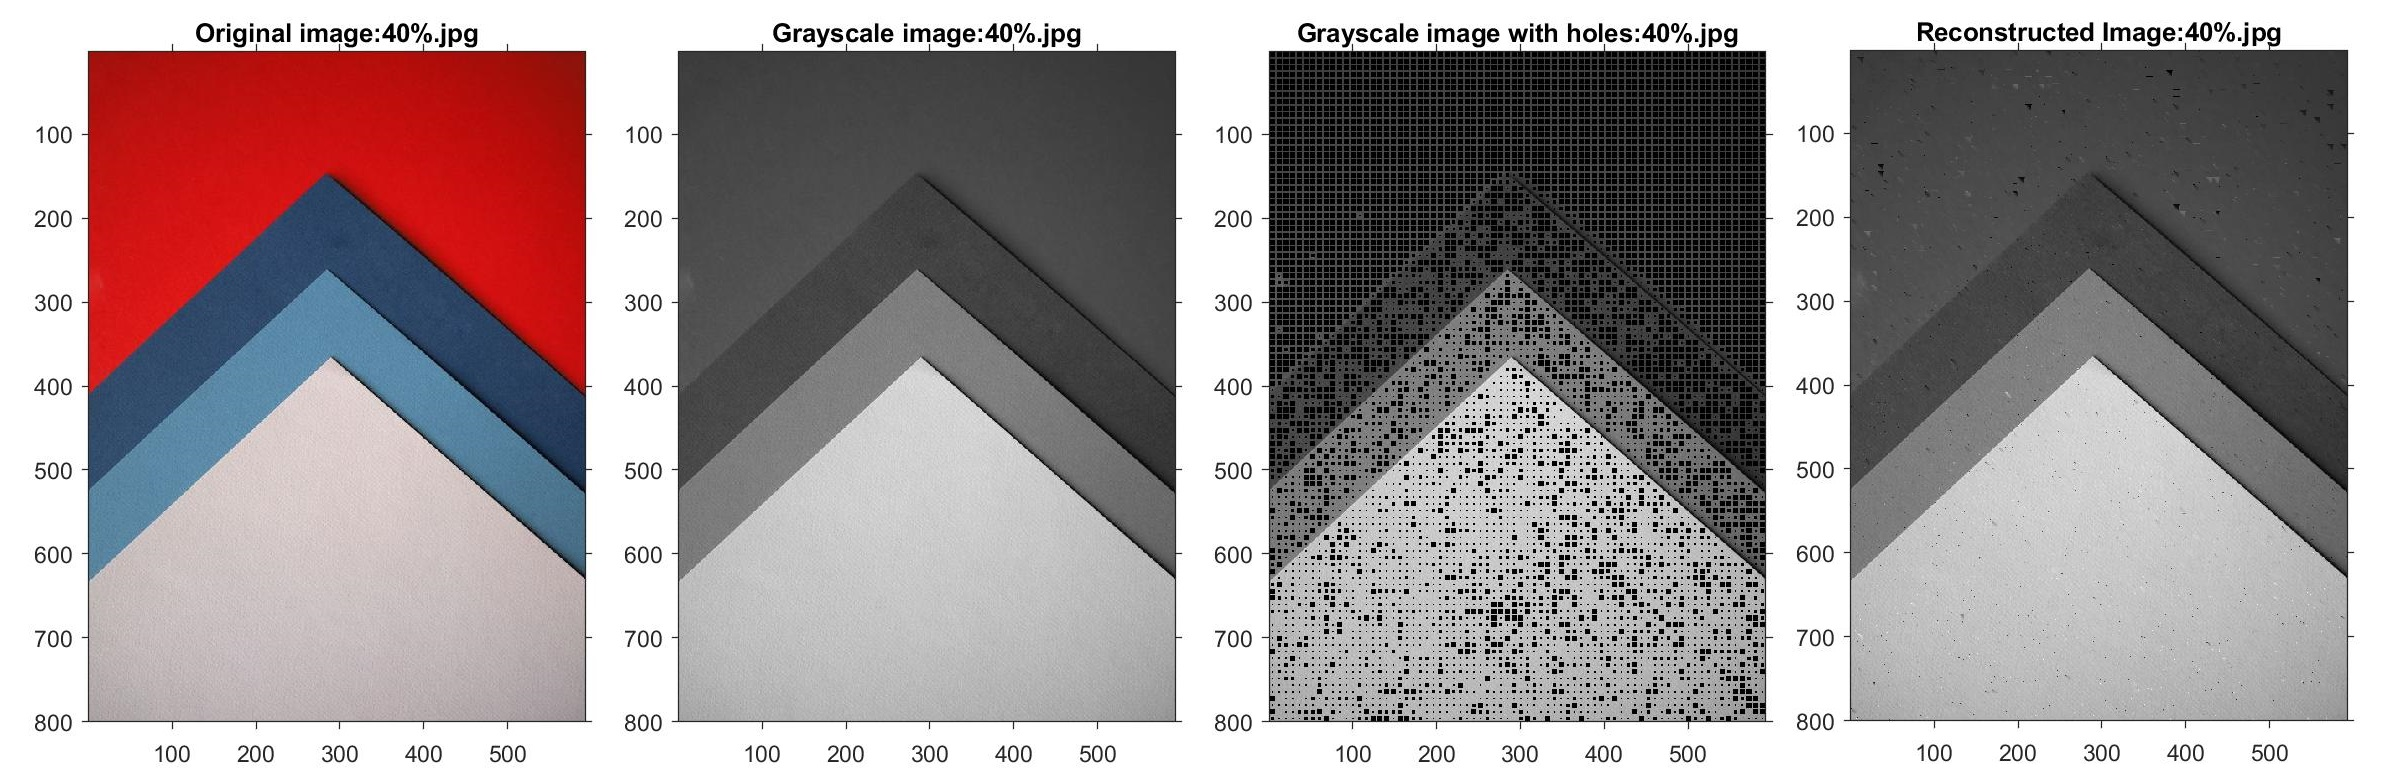
\includegraphics[scale=0.31]{AndrejLisakov40.jpg}
\caption{Andrej Lisakov texture image at 40\% of the original size with 10\% error introduction}
\label{fig:AndrejLisakov40}
\end{figure}

\begin{figure}[!ht]
\center 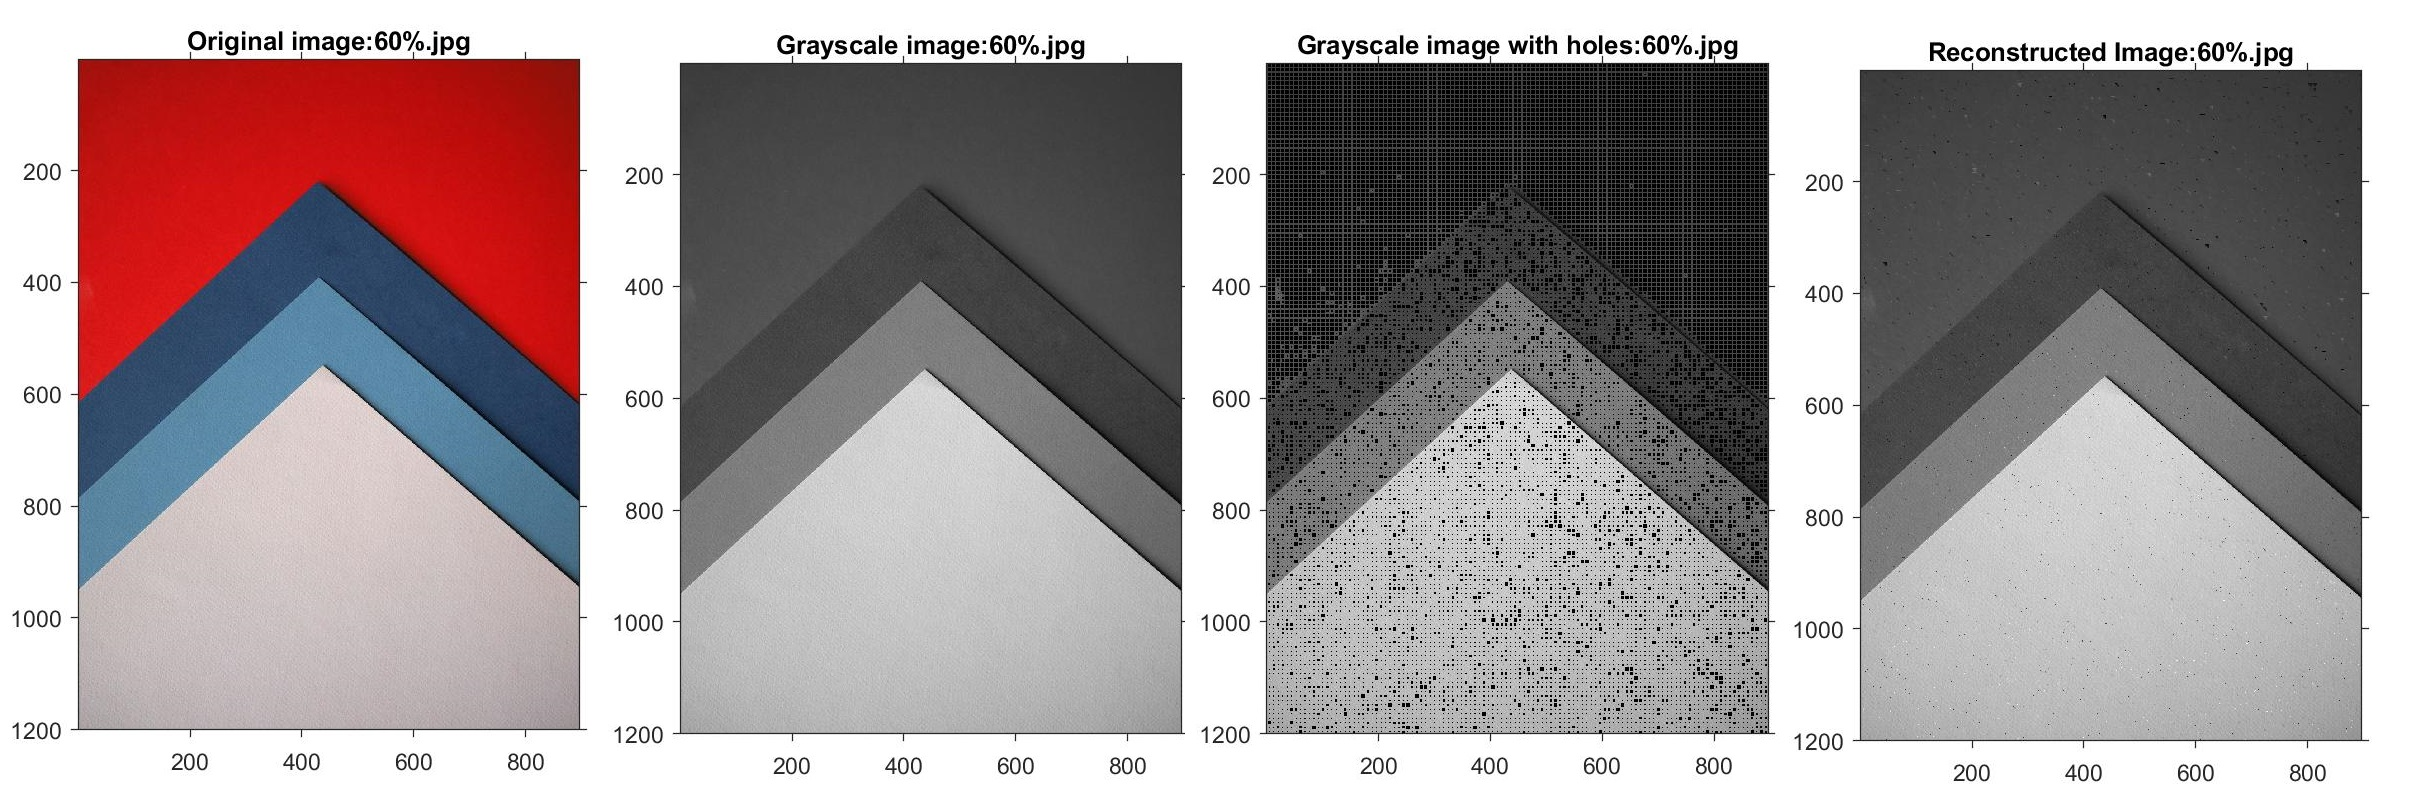
\includegraphics[scale=0.31]{AndrejLisakov60.jpg}
\caption{Andrej Lisakov texture image at 60\% of the original size with 10\% error introduction}
\label{fig:AndrejLisakov60}
\end{figure}

\begin{figure}[!ht]
\center 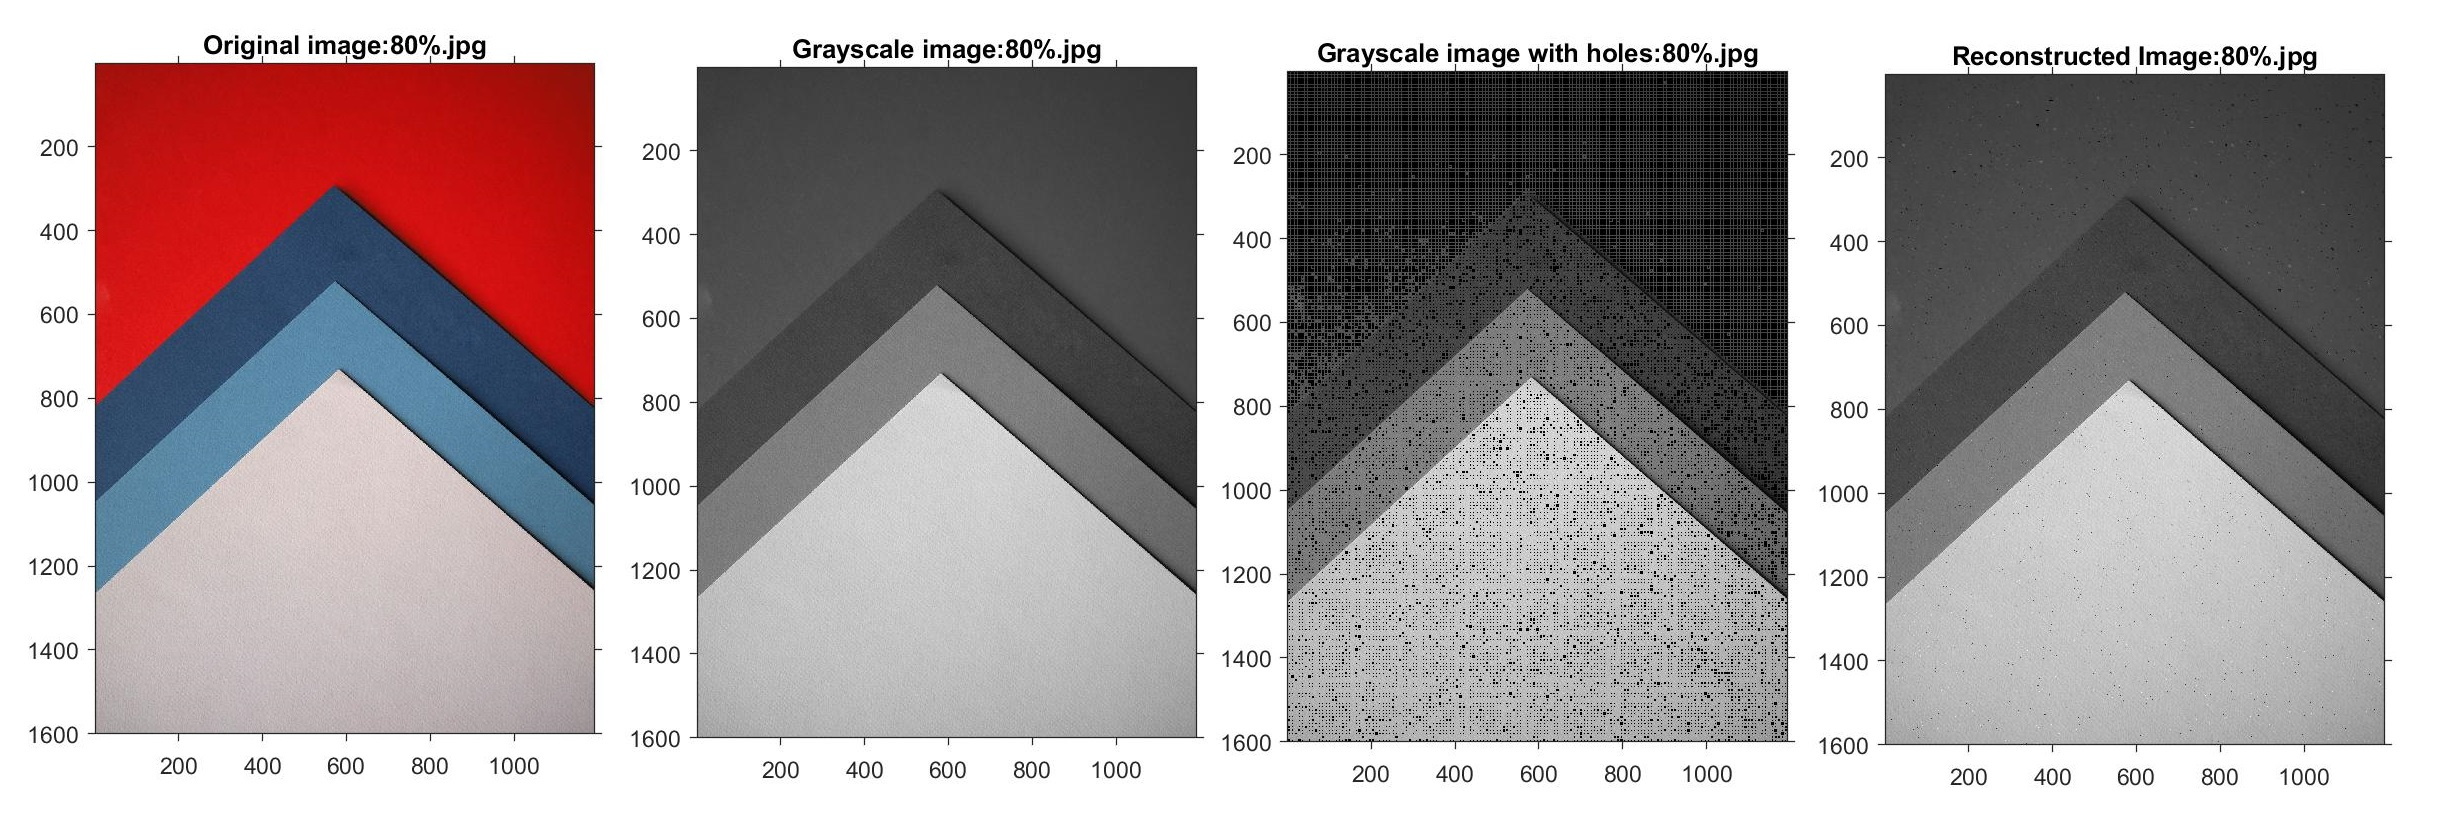
\includegraphics[scale=0.31]{AndrejLisakov80.jpg}
\caption{Andrej Lisakov texture image at 80\% of the original size with 10\% error introduction}
\label{fig:AndrejLisakov80}
\end{figure}

\begin{figure}[!ht]
\center 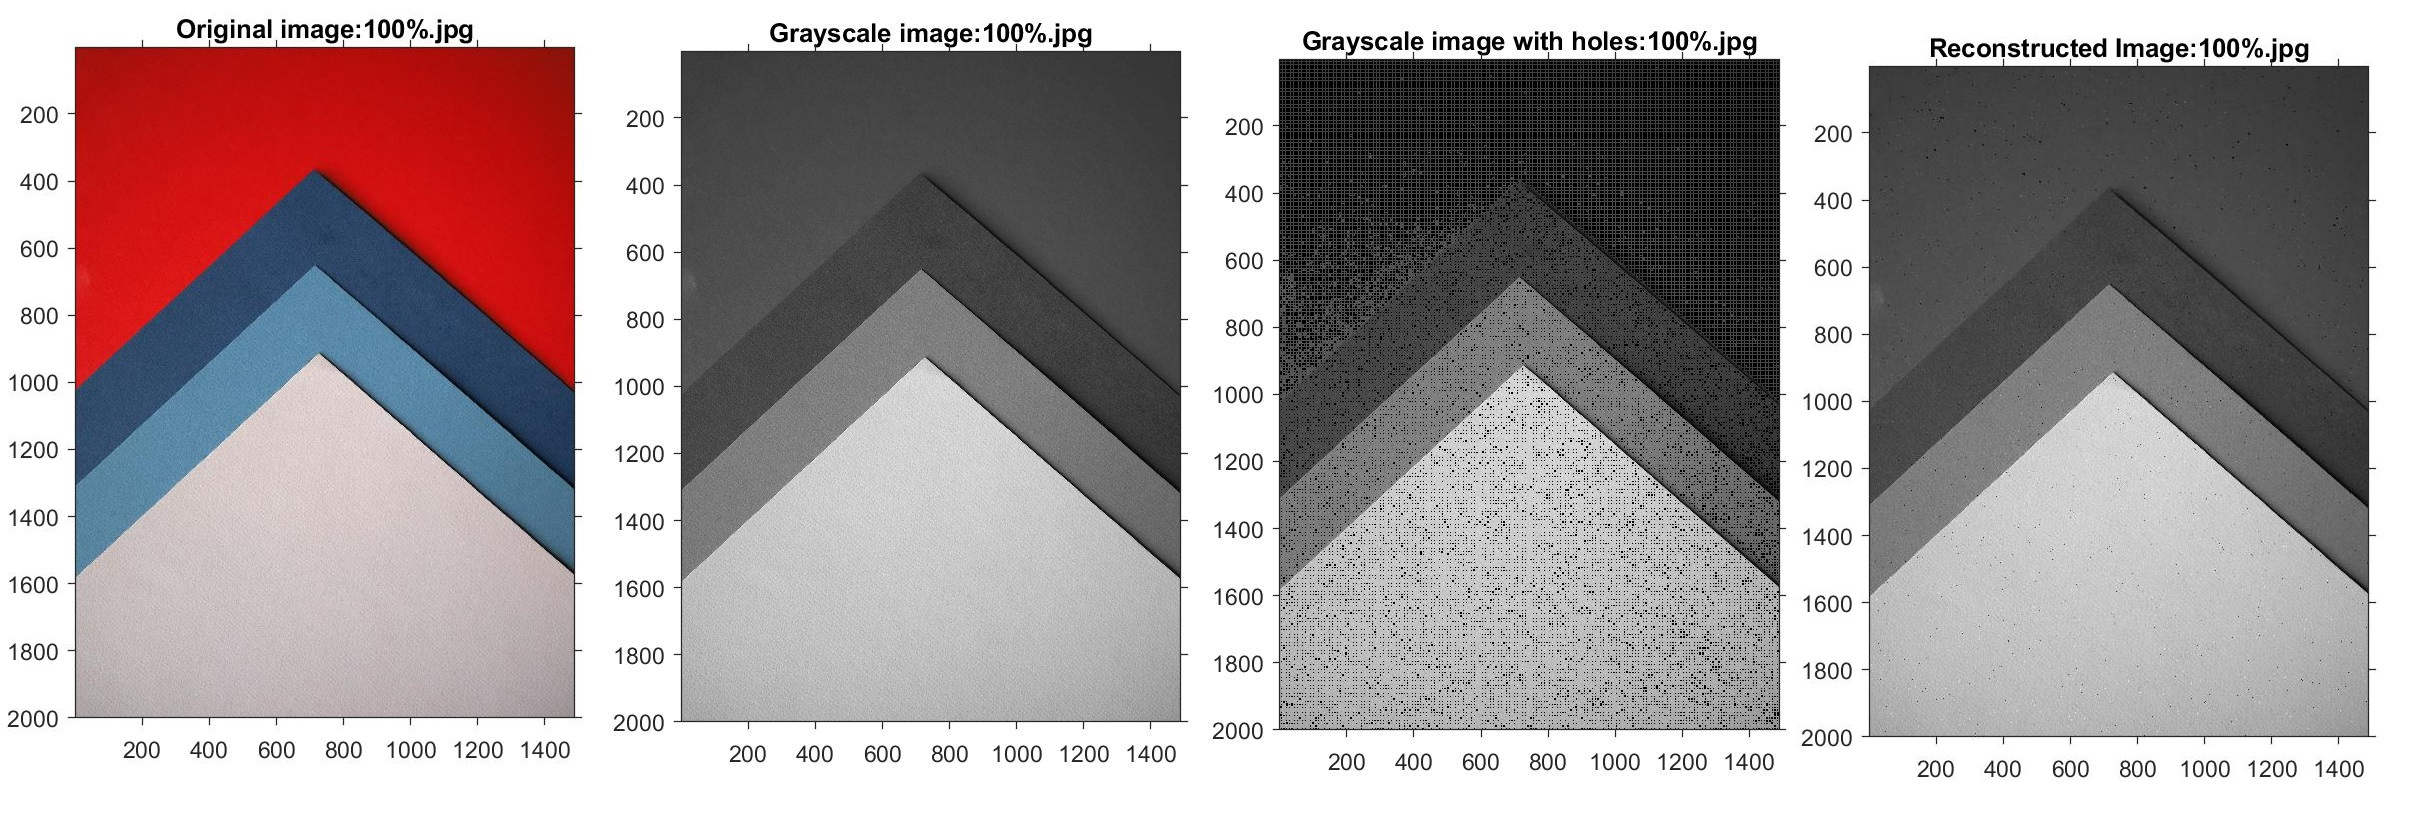
\includegraphics[scale=0.31]{AndrejLisakov100.jpg}
\caption{Andrej Lisakov texture image at 100\% of the original size with 10\% error introduction}
\label{fig:AndrejLisakov100}
\end{figure}

%% Bryan Garces

\begin{figure}[!ht]
\center 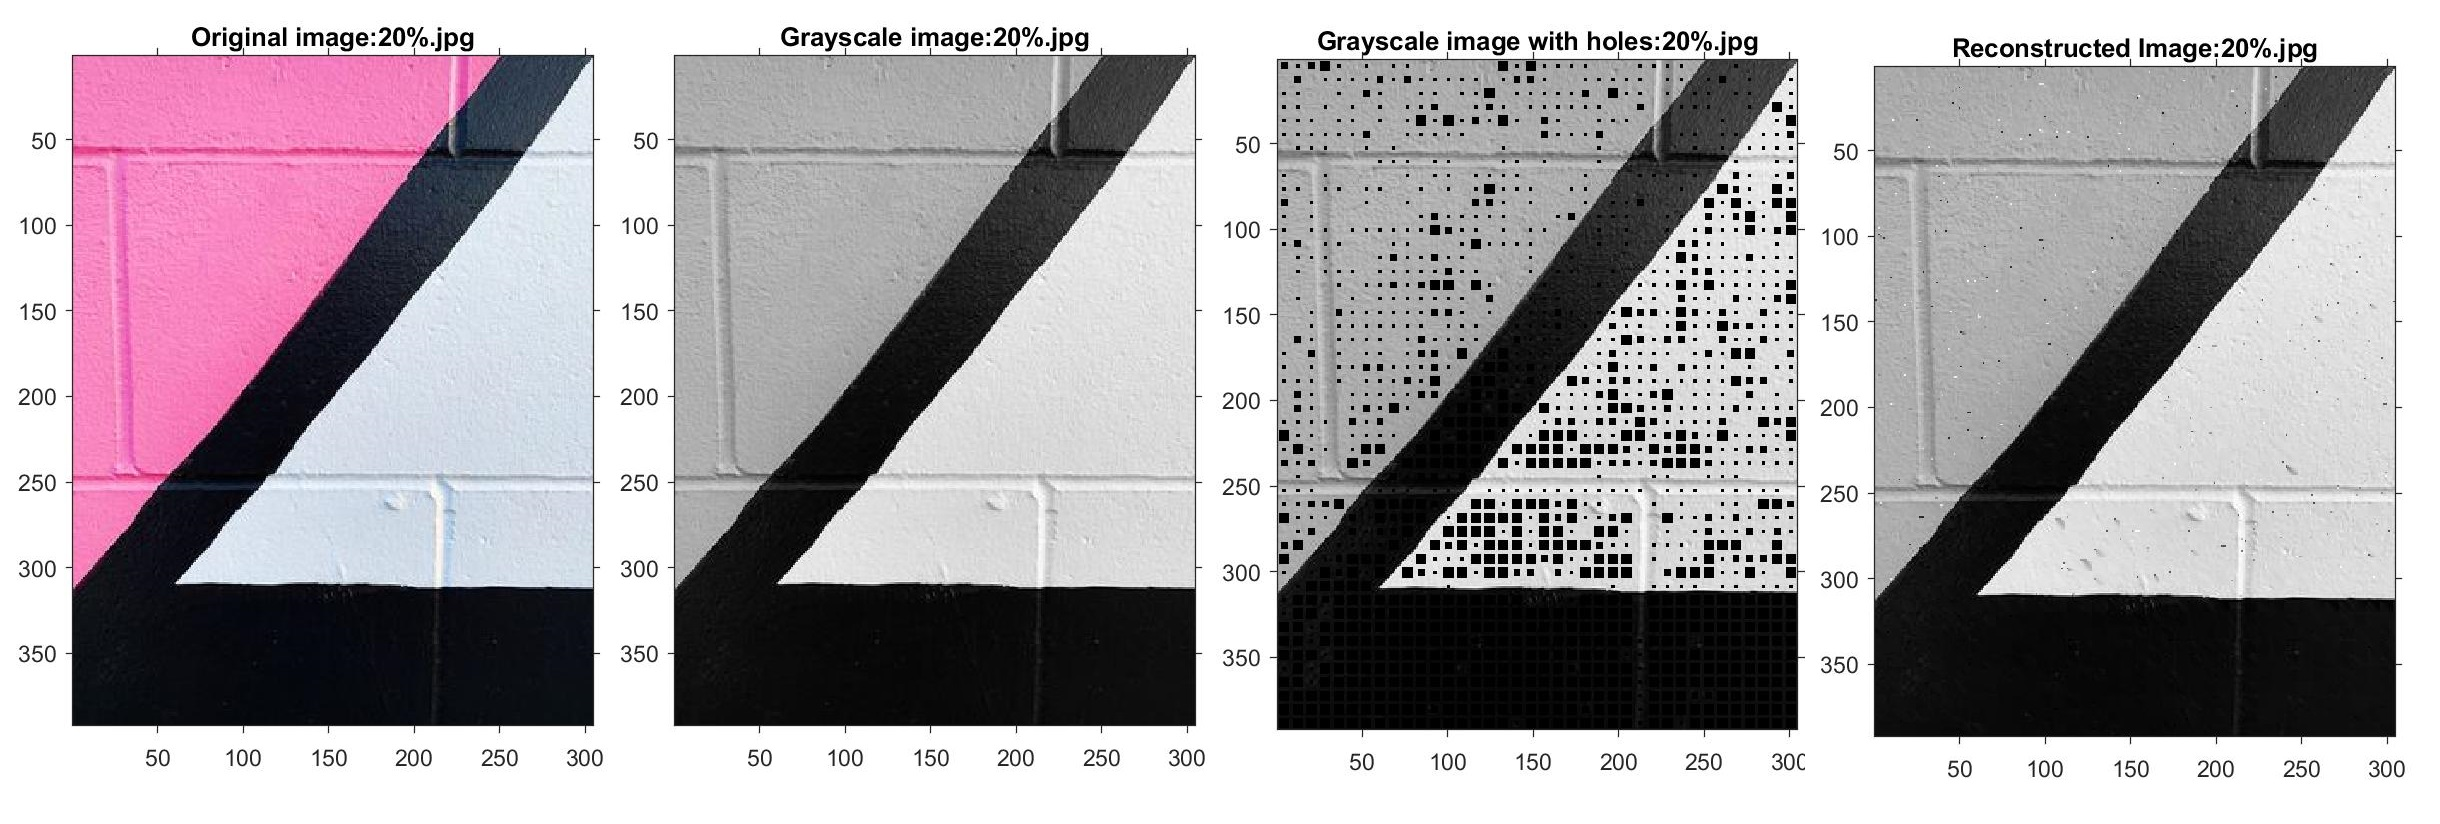
\includegraphics[scale=0.31]{BryanGarces20.jpg}
\caption{Bryan Garces texture image at 20\% of the original size with 10\% error introduction}
\label{fig:BryanGarces20}
\end{figure}

\begin{figure}[!ht]
\center 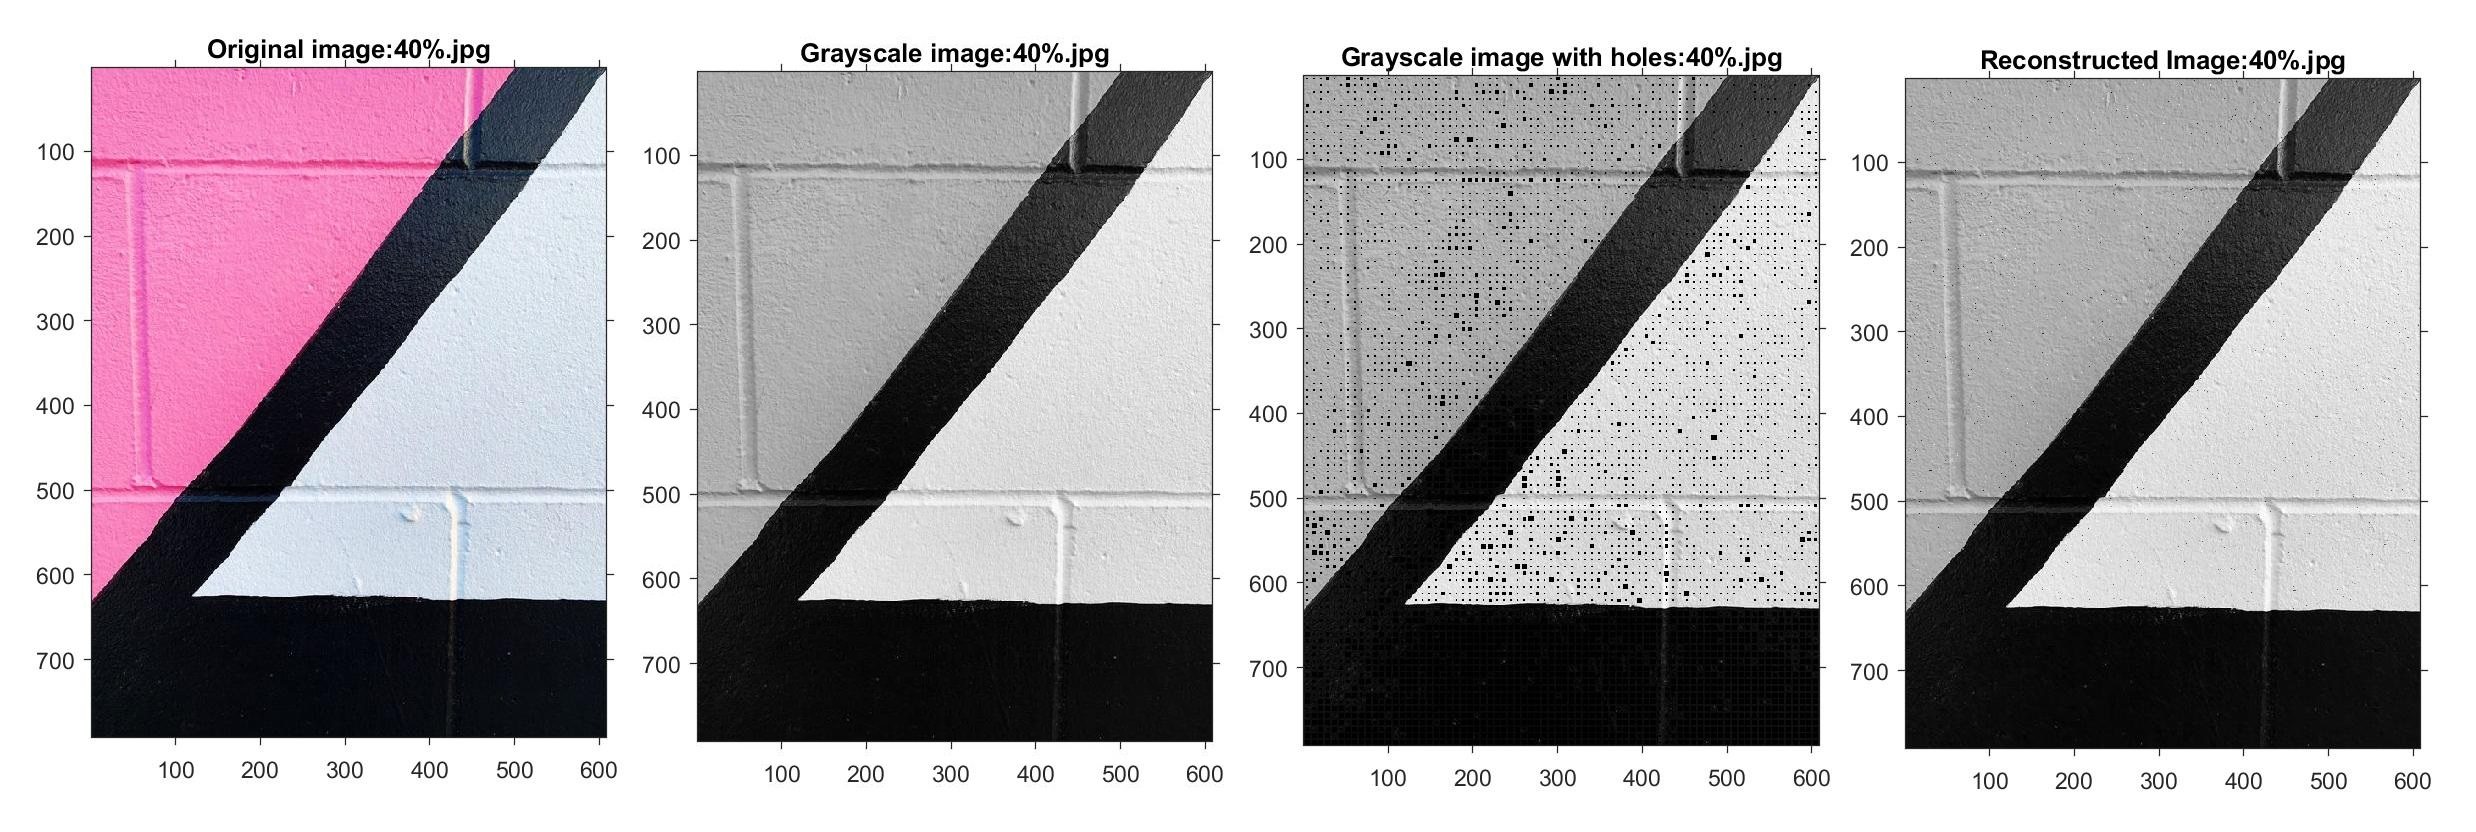
\includegraphics[scale=0.31]{BryanGarces40.jpg}
\caption{Bryan Garces texture image at 40\% of the original size with 10\% error introduction}
\label{fig:BryanGarces40}
\end{figure}

\begin{figure}[!ht]
\center 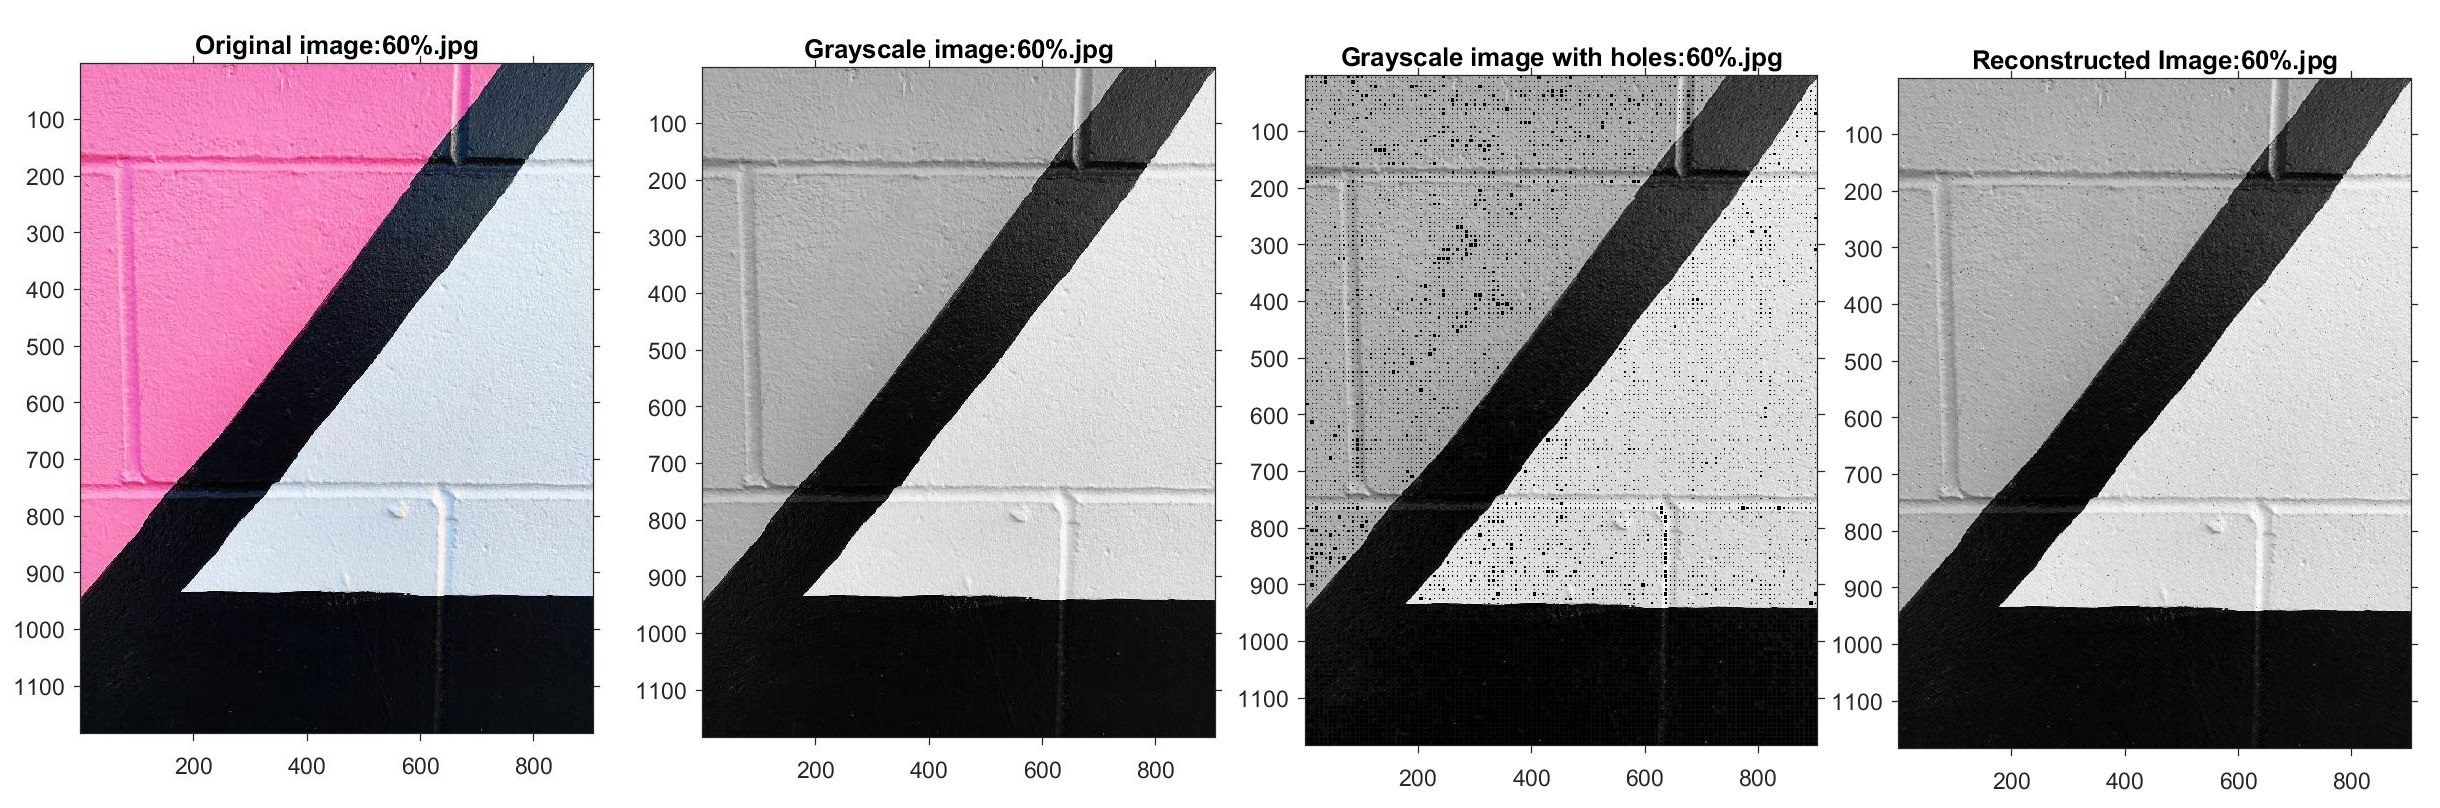
\includegraphics[scale=0.31]{BryanGarces60.jpg}
\caption{Bryan Garces texture image at 60\% of the original size with 10\% error introduction}
\label{fig:BryanGarces60}
\end{figure}

\begin{figure}[!ht]
\center 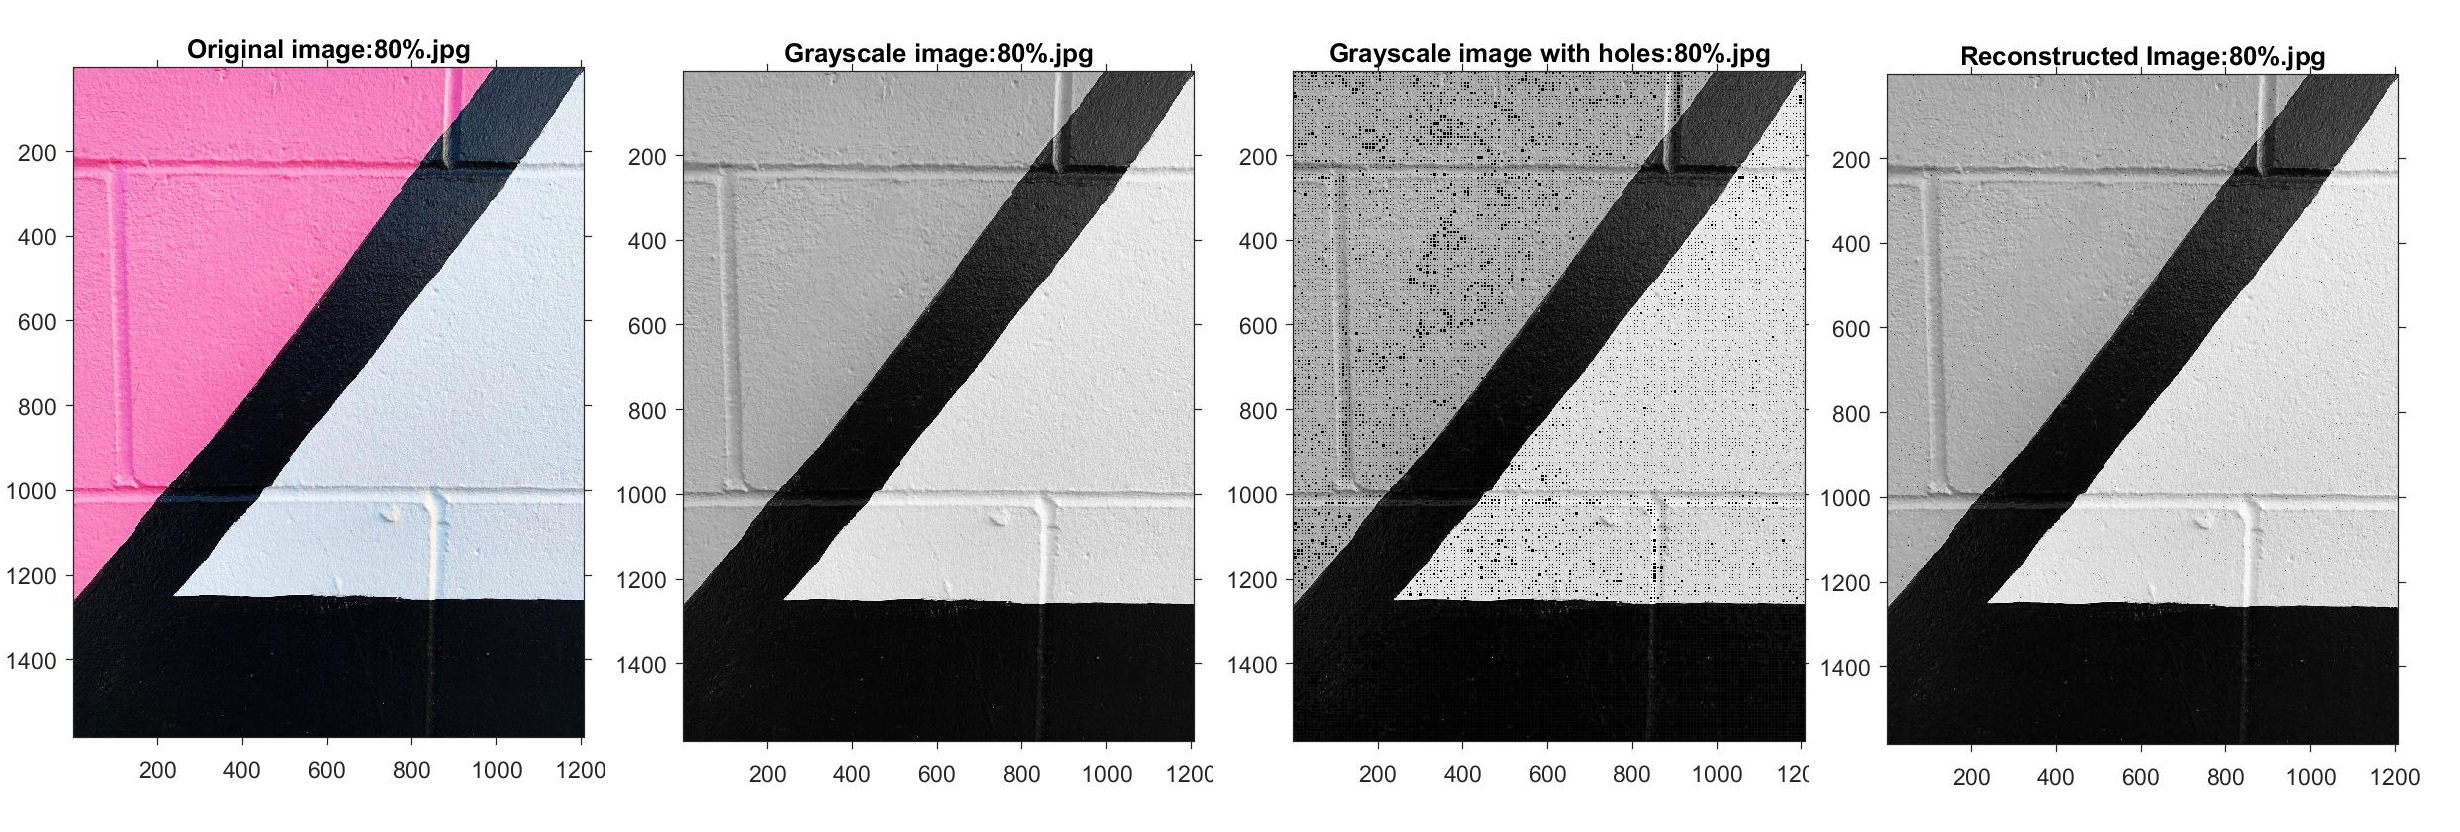
\includegraphics[scale=0.31]{BryanGarces80.jpg}
\caption{Bryan Garces texture image at 80\% of the original size with 10\% error introduction}
\label{fig:BryanGarces80}
\end{figure}

\begin{figure}[!ht]
\center 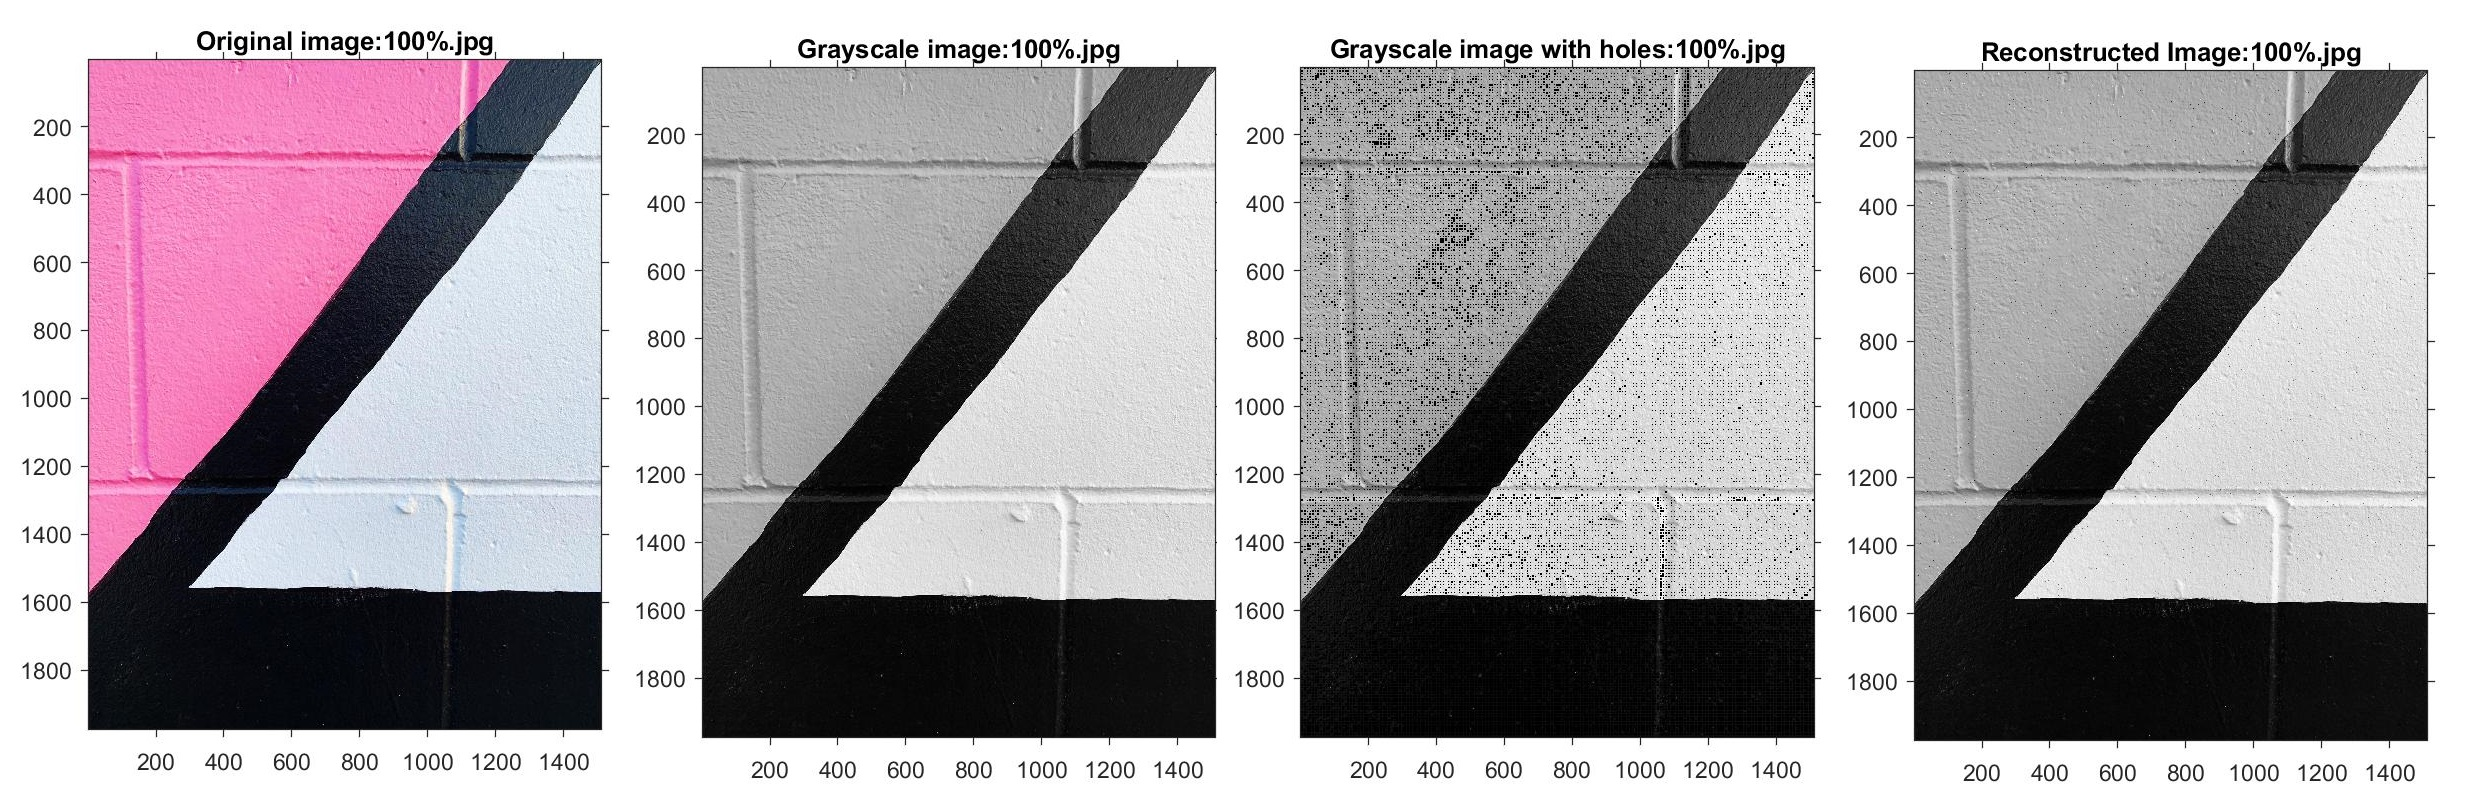
\includegraphics[scale=0.31]{BryanGarces100.jpg}
\caption{Bryan Garces texture image at 100\% of the original size with 10\% error introduction}
\label{fig:BryanGarces100}
\end{figure}

%% Ross Elder

\begin{figure}[!ht]
\center \includegraphics[scale=0.31]{RossElder20.jpg}
\caption{Ross Elder texture image at 20\% of the original size with 10\% error introduction}
\label{fig:RossElder20}
\end{figure}

\begin{figure}[!ht]
\center \includegraphics[scale=0.31]{RossElder40.jpg}
\caption{Ross Elder texture image at 40\% of the original size with 10\% error introduction}
\label{fig:RossElder40}
\end{figure}

\begin{figure}[!ht]
\center \includegraphics[scale=0.31]{RossElder60.jpg}
\caption{Ross Elder texture image at 60\% of the original size with 10\% error introduction}
\label{fig:RossElder60}
\end{figure}

\begin{figure}[!ht]
\center \includegraphics[scale=0.31]{RossElder80.jpg}
\caption{Ross Elder texture image at 80\% of the original size with 10\% error introduction}
\label{fig:RossElder80}
\end{figure}

\begin{figure}[!ht]
\center \includegraphics[scale=0.31]{RossElder100.jpg}
\caption{Ross Elder texture image at 100\% of the original size with 10\% error introduction}
\label{fig:RossElder100}
\end{figure}

%% Vino Li

\begin{figure}[!ht]
\center \includegraphics[scale=0.31]{VinoLi20.jpg}
\caption{Vino Li texture image at 20\% of the original size with 10\% error introduction}
\label{fig:VinoLi20}
\end{figure}

\begin{figure}[!ht]
\center \includegraphics[scale=0.31]{VinoLi40.jpg}
\caption{Vino Li texture image at 40\% of the original size with 10\% error introduction}
\label{fig:VinoLi40}
\end{figure}

\begin{figure}[!ht]
\center \includegraphics[scale=0.31]{VinoLi60.jpg}
\caption{Vino Li texture image at 60\% of the original size with 10\% error introduction}
\label{fig:VinoLi60}
\end{figure}

\begin{figure}[!ht]
\center \includegraphics[scale=0.31]{VinoLi80.jpg}
\caption{Vino Li texture image at 80\% of the original size with 10\% error introduction}
\label{fig:VinoLi80}
\end{figure}

\begin{figure}[!ht]
\center \includegraphics[scale=0.31]{VinoLi100.jpg}
\caption{Vino Li texture image at 100\% of the original size with 10\% error introduction}
\label{fig:VinoLi100}
\end{figure}

%%
%%